\documentclass[a4paper,11pt,openright]{report}
\usepackage[utf8]{inputenc}
\usepackage[italian]{babel}
\usepackage{amssymb}
\usepackage{amsmath}
\usepackage{amsthm}
\usepackage{float}
\usepackage{afterpage}
\usepackage{graphicx}
\usepackage[toc,page]{appendix}
\usepackage{biblatex}
%\usepackage[margin=1in]{geometry}
\renewcommand{\appendixtocname}{Appendice}
\renewcommand{\appendixpagename}{Appendice}
\newtheorem{teo}{Teorema}[section]
\newtheorem{lemma}[teo]{Lemma}
\newtheorem{osservazione}[teo]{Osservazione}
\newtheorem{esempio}[teo]{Esempio}
\newtheorem{ipotesi} [teo]{Ipotesi}
\newtheorem{notazione}[teo]{Notazione}
\newtheorem{corollario}[teo]{Corollario}
\newtheorem{proposizione}[teo]{Proposizione}
\newtheorem{euristica}[teo]{Euristica}
\newtheorem{definizione}[teo]{Definizione}
\newtheorem{notabene}[teo]{N.B.}

\newcommand\blankpage{
	\null
	\thispagestyle{empty}
	\newpage
	}



\begin{document}

\chapter{Studio Numerico}

\section{Kuramoto-Shinomoto-Sakaguchi MV-SDE}
Scriviamo, in primis, la MV-SDE relativa al modello che andremo ad analizzare, ovvero il modello di Kuramoto-Shinomoto-Sakaguchi:
\[
dX_t = \left( {\rm I\!E}[\sin(X_t)] \cos(X_t) - {\rm I\!E}[\cos(X_t)]\sin(X_t) \right) dt + \sigma dW_t , \ \ \ X_0=x_0, 
\]
dove nel nostro caso $\sigma = 0.5$ e $x_0 = 0.5$. Da questa equazione differenziale si evince facilmente che:
\begin{itemize}
\item K = 3, d = 1 e q = 1,
\item $\varphi(x)=(1, \sin x, \cos x)$, 
\item $\alpha(t,x)=(0, \cos x, -\sin x)^T$, 
\item $\beta(t,x)=(\sigma, 0, 0)^T$.
\end{itemize}
Il nostro studio, i risultati numerici e le osservazioni che emergono sono ottenuti dal lavoro di due macro funzioni, entrambe volte al calcolo approssimato dei valori di ${\rm I\!E}[\sin(X_t)]$ e ${\rm I\!E}[\cos(X_t)]$. 
\begin{itemize}
\item[-] La prima, che usiamo per ottenere la soluzione che svolgerà per noi il ruolo di benchmark, è l'ormai noto metodo Eulero - Monte Carlo. Esso consiste nell'approssimare i due valori attesi in questione mediante una media diretta di $M_1 = 10^6$ simulazioni di processi $(X_t)_{t=0, \cdots T}$ ottenuti dividendo l'intervallo $[0,T]$ in $N_1$ step temporali e applicando in ciascuno di essi il metodo di Eulero. Nello specifico il Metodo di Eulero calcola gli $N+1$ valori di un processo discretizzato ottenendo, ad ogni passo, il valore al tempo $t$ dal valore del processo al tempo precedente e dal valore dello step temporale $h$, secondo la formula:
\[
X_{t+1} = X_t + \mathrm{drift}(t) \cdot h + \mathrm{diffusione}(t) \cdot \sqrt{h} \cdot W, 
\]
dove $W$ è il valore della realizzazione di una Normale Standard.
Nel nostro caso gli step temporali sono tutti equivalenti in quanto suddividiamo l'intervallo $[0,T]$ in punti equispaziati. Mettiamo in evidenza che la funzione in questione è strutturata in modo da poter essere applicata anche alla categoria di SDEs di McKean-Vlasov, per le quali il metodo di Eulero al passo $t+1$ richiede che siano noti, all'interno delle parti di drift e diffusione, i valori attesi cercati, al tempo $t$. Per ottenerli sfruttiamo anche in questo caso una media sulle $M_1$ simulazioni delle realizzazioni dei processi al tempo $t$. 
\item[-] La seconda è il metodo di Discesa Stocastica del Gradiente descritto nel capitolo precedente. Questa produrrà i polinomi $(\mathcal{L}(a))_1(t)$ e $(\mathcal{L}(a))_2(t)$ che saranno rispettivamente le  approssimazioni di ${\rm I\!E}[\sin(X_t)]$ di ${\rm I\!E}[\cos(X_t)]$, risolvendo il nostro problema di ottimizzazione. Per quanto concerne la scelta dello spazio dei polinomi, i due output sono calcolati nella base di quelli ortogonali di Lagrange. La dimensione $n$ dello spazio dei polinomi verrà fatta variare, mentre ciascun elemento della base è della forma: 
\[
g_i(t):=\prod_{j \leq n \ e  \ j\neq n} \left( \frac{t - t_j}{t_i - t_j} \right), \text{ con nodi di Chebyshev } \cfrac{T}{2} + \cfrac{T}{2} \cos \left( \cfrac{2k + 1}{2n +2} \pi \right).
\]
Anche in questo caso sarà necessario ricorre agli $N$ step di Eulero per trovare la soluzione delle SDEs. Questa volta il metodo di Eulero per la simulazione di $Z(\xi , W)$ e di $\left( Z^a(\tilde{\xi} , \tilde{W}), \partial_{a_{h,j}} Z^a(\tilde{\xi} , \tilde{W}) \right)$ dovrà portare avanti 4 processi simultaneamente: $(X_t)_{t=0, \cdots T}$ e $(Z_t)_{t=0, \cdots T}$ monodimensionali e le due $(Y_t)^{(1,2)}_{t=0, \cdots T}$ $n+1$ dimensionali. Inoltre sarà necessario usare a ogni passo il valore ottenuto per il processo $X$ per poter calcolare le due $Y^{(1,2)}$. Notiamo che $X$ e $Z$ implementano lo step di Eulero al medesimo modo della funzione precedente, ma con due realizzazioni differenti del Browniano. In questo algoritmo semplificato le mappe $\textbf{h}$ e $ H $ sono prese rispettivamente come l'identità e la funzione nulla. Riprendendo i valori delle funzioni dei coefficienti per la MV-SDE relativa al modello di Kuramoto-Shninomoto-Sakaguchi si ottiene che nello specifico le equazioni diventano:
\[
dZ_t = \left( (\mathcal{L}a)_1(t) \cos(Z_t) - (\mathcal{L}a)_2(t) \sin(Z_t) \right) dt + \sigma dW_t, 
\]
\[
dY^{j,1}_t = \left( g_j(t) \cos(Z_t) - Y^{j,1}_t \left( (\mathcal{L}a)_1(t)\sin(Z_t) + (\mathcal{L}a)_2(t)\cos(Z_t)\right) \right)dt, 
\]
\[
dY^{j,2}_t = \left( -g_j(t) \sin(Z_t) - Y^{j,2}_t \left( (\mathcal{L}a)_1(t)\sin(Z_t) + (\mathcal{L}a)_2(t)\cos(Z_t)\right) \right)dt, 
\]
con $Z_0 = X_0$, $Y^{j,1}_0 = 0 $ e $Y^{j,2}_0 = 0$ e per $j = 0, \cdots , n$. Questi processi sono necessari per calcolare la realizzazione del gradiente per la Discesa Stocastica, ovvero la variabile aleatoria $v$. Avendo suddiviso il tempo in $N$ step temporali e  approssimato l'integrale con una sommatoria la scrittura della $v$ della nostra funzione, componente per componente, è la seguente:
\begin{align*}
v_{j,1}&(a; W; \tilde{W}) = \\
&2 h \sum_{t=0}^{N} \left[ \left( \sin(Z^a_t(W)) - (\mathcal{L}a)_1(t) \right) \cdot \left( \cos(Z^a_t(\tilde{W})) Y_t^{a;j,1}(\tilde{W}) - g_j(t) \right) \right.\\
&\left.+ \left( \cos(Z^a_t(W)) - (\mathcal{L}a)_2(t) \right) \cdot \left( -\sin(Z^a_t(\tilde{W})) Y_t^{a;j,1}(\tilde{W}) \right)\right],
\end{align*}
\begin{align*}
v_{j,2}&(a; W; \tilde{W}) = \\
&2 h \sum_{t=0}^{N} \left[ \left( \sin(Z^a_t(W)) - (\mathcal{L}a)_1(t) \right) \cdot \left( \cos(Z^a_t(\tilde{W})) Y_t^{a;j,2}(\tilde{W}) \right) \right.\\
&\left.+ \left( \cos(Z^a_t(W)) - (\mathcal{L}a)_2(t) \right) \cdot \left( -\sin(Z^a_t(\tilde{W})) Y_t^{a;j,2}(\tilde{W}) - g_j(t) \right)\right],
\end{align*}
con $j = 0, \cdots , n$.
Concludiamo mettendo in evidenza che prima di restituire il valore $v$, questa funzione fa una media di $M$ realizzazioni ottenute corrispondenti ad altrettante simulazioni indipendenti di moti Browniani. Se tale parametro è lasciato a 1 il metodo è un classico metodo SGD, ma se portato a $\infty$ porta a un metodo GD, ovvero di discesa deterministica. Questo strategia, chiamata Mini Batch, è al centro delle analisi numeriche che abbiamo eseguito. Infine, per quanto concerne la scelta dei $learing \ rates,$ necessari per il calcolo di $v$ ad ogni iterazione, scegliamo $\eta_m = \cfrac{r_0}{(m + 1)^\rho}$, basandoci anche sui risultati di \cite{fehrman2020convergence}, dove i coefficienti $r_0 \in (0, +\infty)$ e $\cfrac{1}{2} < \rho \leq 1$ sono stati fatti variare nel corso dello studio numerico. 
\end{itemize}

\section{Tabelle e Grafici}
Lo scopo della nostra analisi è quello di trovare il numero di iterazioni necessarie per portare a convergenza il metodo di Discesa del Gradiente. A tal proposito esplicitiamo il criterio d'arresto per l'iterazione di $a_m$: fissati $\gamma_{1,bench}$ e $\gamma_{2, bench}$ ottenuti dalla prima funzione, le iterazioni terminano quando
\[ 
\frac{\|\sum_{i=0}^n (a_1)_i g_i - \gamma_{1, bench} \|_{L_2}}{\| \gamma_{1, bench}\|_{L_2}} < 1\% \ \ \ \mbox{ e } \ \ \ \frac{\|\sum_{i=0}^n (a_2)_i g_i - \gamma_{2, bench} \|_{L_2}}{\| \gamma_{2, bench}\|_{L_2}} < 1\%.
\]
Pertanto la seconda funzione, descritta nella sezione precedente, produrrà come output una soluzione avente errore relativo dell'$1 \% $, in norma $L_2$, rispetto alla soluzione benchmark. Per rendere più generali e corretti possibile tali risultati, ripetiamo lo stesso test al variare di: istante finale $ T = 0.5, 1, 2, 4$; dimensione dello spazio dei polinomi $ n = 3, 4, 5, 6 $; e valori dei parametri $\rho = 0.6, 0.7, 0.8, 0.9$ e $r_0 = 1, 5, 10$ dei \emph{learning rates}. Specifichiamo che, al fine di ottenere lo stesso ordine di errore nel metodo di Eulero e pertanto mantenere costante in tutti i test il parametro $h$, suddividiamo l'intervallo $[0,T]$ in $N_1 = 50, 100, 200, 400$ step, rispettivamente ai valori di $T$ appena elencati. In particolare ripetiamo per ciascuna casistica lo stesso test $10$ volte e riportato: i tempi di convergenza medi, una tabella che per ogni combinazione di $\rho$ e $r_0$ mostra il numero minore, massimo e medio di iterazioni di convergenza e i grafici delle soluzioni approssimate. I grafici che mostreremo saranno quelli relativi ai valori di $\rho$ e $r_0$ che nelle tabelle presentano minor numero di iterazioni medie, per ogni combinazione dei parametri $T$, $n$ e $M$. Il tutto è eseguito al variare del valore del Mini Batch $M = 1, 10, 10^2, 10^3, 10^4$ e del grado dei polinomi $n$. Raggruppiamo tali tabelle e grafici in sezioni in base al valore di $T$.

\begin{notabene}
Quando nelle tabelle compaiono valori come "overflow" o $49999$ significano rispettivamente che durante l'esecuzione del programma è avvenuto un $overflow$, ovvero si è raggiunto il limite della capacità di storage del valore (quindi un numero troppo grande); mentre il secondo significa che l'algoritmo non è arrivato a convergenza entro le $50000$ iterazioni imposte come threshold.
\end{notabene}

\begin{notabene}
Per quanto concerne i primi tre valori di $M$, ovvero $M = 1, 10, 100$, il confronto col benchmark avviene ogni dieci iterazioni, così da contenere i tempi di esecuzione. Mentre per gli ultimi due casi, ovvero $M = 1000, 10000$, tale controllo avviene ogni step.
\end{notabene}

\begin{notabene}
Specifichiamo che gli algoritmi sono stati scritti nel linguaggio di programmazione Python, nello specifico nell'applicazione web Jupyter Notebook per la creazione e la condivisione di documenti computazionali. Per quanto concerne i tempi di esecuzione dell'algoritmo, scrivo di seguito le specifiche della macchina sulla quale ho eseguito i test:

Processore	Intel(R) Core(TM) i5-8250U CPU @ 1.60GHz   1.80 GHz 

RAM installata	8,00 GB (7,90 GB utilizzabile) 


Tipo sistema	Sistema operativo a 64 bit, processore basato su x64 
\end{notabene}
\[
\]
\newpage
\section{T = 0.5}
\section*{Caso n = 3}  
\begin{table}[H]
\centering
\addtolength{\leftskip}{-1.5cm}
\addtolength{\rightskip}{-1.5cm}
\begin{tabular}{|c|lll|}
\hline
$ $ & $r_0 = 1$ & $r_0 = 5$ & $r_0 = 10$ \\
\hline
$\rho = 0.6$ & 0.95 & 1.48 & 4.34 \\

$\rho = 0.7$ & 2.17 & 1.5 & 1.80 \\

$\rho = 0.8$ & 2.82 & 1.23 & 1.96 \\

$\rho = 0.9$ & 19.22 & 1.14 & 1.35 \\
\hline
\end{tabular}
\caption{Average execution
 times (in seconds $s$) with $M = 1$}
\end{table}
\begin{table}[H]
\centering
\addtolength{\leftskip}{-1.5cm}
\addtolength{\rightskip}{-1.5cm}
\begin{tabular}{|c|lllllllll|}
\hline
$ $ & $r_0 = 1$ & $r_0 = 1$ & $r_0 = 1$ & $r_0 = 5$ & $r_0 = 5$ & $r_0 = 5$ & $r_0 = 10$ & $r_0 = 10$ & $r_0 = 10$  \\
$ $ & min & max & average & min & max & average & min & max & average \\ 
\hline
$\rho = 0.6$ & 80 & 490 & 278 & 170 & 720 & 438 & 630 & 2500 & 1281 \\

$\rho = 0.7$ & 30 & 2380 & 639 & 140 & 730 & 442 & 80 & 1050 & 532\\

$\rho = 0.8$ & 40 & 2070 & 831 & 100 & 1240 & 362 & 210 & 1170 & 581\\

$\rho = 0.9$ & 400 & 20930 & 5668 & 160 & 600 & 338 & 150 & 1020 & 403\\
\hline
\end{tabular}
\caption{Number of iterations $m$ to achieve convergence with $M = 1$}
\end{table}
\begin{table}[H]
\centering
\addtolength{\leftskip}{-1.5cm}
\addtolength{\rightskip}{-1.5cm}
\begin{tabular}{|c|lll|}
\hline
$ $ & $r_0 = 1$ & $r_0 = 5$ & $r_0 = 10$ \\
\hline
$\rho = 0.6$ & 0.41 & 0.32 & 0.74 \\

$\rho = 0.7$ & 0.48 & 0.38 & 0.44 \\

$\rho = 0.8$ & 1.25 & 0.34 & 0.40 \\

$\rho = 0.9$ & 2.46 & 0.35 & 0.41 \\
\hline
\end{tabular}
\caption{Average execution
 times (in seconds $s$) with $M = 10$}
\end{table}
\begin{table}[H]
\centering
\addtolength{\leftskip}{-1.5cm}
\addtolength{\rightskip}{-1.5cm}
\begin{tabular}{|c|lllllllll|}
\hline
$ $ & $r_0 = 1$ & $r_0 = 1$ & $r_0 = 1$ & $r_0 = 5$ & $r_0 = 5$ & $r_0 = 5$ & $r_0 = 10$ & $r_0 = 10$ & $r_0 = 10$  \\
$ $ & min & max & average & min & max & average & min & max & average \\ 
\hline
$\rho = 0.6$ & 20 & 230 & 105 & 10 & 150 & 82 & 60 & 510 & 192\\

$\rho = 0.7$ & 30 & 400 & 124 & 30 & 190 & 99 & 30 & 270 & 113\\

$\rho = 0.8$ & 30 & 1160 & 322 & 30 & 180 & 88 & 60 & 170 & 104\\

$\rho = 0.9$ & 20 & 2660 & 635 & 20 & 220 & 89 & 30 & 290 & 106\\
\hline
\end{tabular}
\caption{Number of iterations $m$ to achieve convergence with $M = 10$}
\end{table}
\begin{table}[H]
\centering
\addtolength{\leftskip}{-1.5cm}
\addtolength{\rightskip}{-1.5cm}
\begin{tabular}{|c|lll|}
\hline
$ $ & $r_0 = 1$ & $r_0 = 5$ & $r_0 = 10$ \\
\hline
$\rho = 0.6$ & 0.11 & 0.14 & 0.19 \\

$\rho = 0.7$ & 0.18 & 0.12 & 0.17 \\

$\rho = 0.8$ & 0.36 & 0.15 & 0.17 \\

$\rho = 0.9$ & 0.53 & 0.14 & 0.12 \\
\hline
\end{tabular}
\caption{Average execution
 times (in seconds $s$) with $M = 100$}
\end{table}
\begin{table}[H]
\centering
\addtolength{\leftskip}{-1.5cm}
\addtolength{\rightskip}{-1.5cm}
\begin{tabular}{|c|lllllllll|}
\hline
$ $ & $r_0 = 1$ & $r_0 = 1$ & $r_0 = 1$ & $r_0 = 5$ & $r_0 = 5$ & $r_0 = 5$ & $r_0 = 10$ & $r_0 = 10$ & $r_0 = 10$  \\
$ $ & min & max & average & min & max & average & min & max & average \\ 
\hline
$\rho = 0.6$ & 10 & 30 & 17 & 10 & 50 & 23 & 10 & 80 & 30\\

$\rho = 0.7$ & 10 & 60 & 29 & 10 & 40 & 19 & 10 & 70 & 27\\

$\rho = 0.8$ & 20 & 270 & 58 & 10 & 70 & 24 & 10 & 50 & 27\\

$\rho = 0.9$ & 20 & 470 & 86 & 10 & 50 & 22 & 10 & 40 & 20\\
\hline
\end{tabular}
\caption{Number of iterations $m$ to achieve convergence with $M = 100$}
\end{table}
\begin{table}[H]
\centering
\addtolength{\leftskip}{-1.5cm}
\addtolength{\rightskip}{-1.5cm}
\begin{tabular}{|c|lll|}
\hline
$ $ & $r_0 = 1$ & $r_0 = 5$ & $r_0 = 10$ \\
\hline
$\rho = 0.6$ & 0.34 & 0.09 & 0.26 \\

$\rho = 0.7$ & 0.42 & 0.09 & 0.20 \\

$\rho = 0.8$ & 0.52 & 0.10 & 0.18 \\

$\rho = 0.9$ & 0.84 & 0.09 & 0.16 \\
\hline
\end{tabular}
\caption{Average execution
 times (in seconds $s$) with $M = 1000$}
\end{table}
\begin{table}[H]
\centering
\addtolength{\leftskip}{-1.5cm}
\addtolength{\rightskip}{-1.5cm}
\begin{tabular}{|c|lllllllll|}
\hline
$ $ & $r_0 = 1$ & $r_0 = 1$ & $r_0 = 1$ & $r_0 = 5$ & $r_0 = 5$ & $r_0 = 5$ & $r_0 = 10$ & $r_0 = 10$ & $r_0 = 10$  \\
$ $ & min & max & average & min & max & average & min & max & average \\ 
\hline
$\rho = 0.6$ & 7 & 13 & 9.1 & 2 & 4 & 2.5 & 6 & 11 & 7.1\\

$\rho = 0.7$ & 9 & 15 & 11.4 & 2 & 5 & 2.4 & 5 & 8 & 5.6\\

$\rho = 0.8$ & 11 & 27 & 14.1 & 2 & 6 & 2.7 & 4 & 7 & 5\\

$\rho = 0.9$ & 14 & 35 & 23 & 2 & 5 & 2.4 & 4 & 6 & 4.4\\
\hline
\end{tabular}
\caption{Number of iterations $m$ to achieve convergence with $M = 1000$}
\end{table}
\begin{table}[H]
\centering
\addtolength{\leftskip}{-1.5cm}
\addtolength{\rightskip}{-1.5cm}
\begin{tabular}{|c|lll|}
\hline
$ $ & $r_0 = 1$ & $r_0 = 5$ & $r_0 = 10$ \\
\hline
$\rho = 0.6$ & 3.48 & 0.90 & 2.69 \\

$\rho = 0.7$ & 4.23 & 0.90 & 2.23 \\

$\rho = 0.8$ & 5.14 & 0.90 & 1.79 \\

$\rho = 0.9$ & 7.21 & 0.94 & 1.79 \\
\hline
\end{tabular}
\caption{Average execution
 times (in seconds $s$) with $M = 10000$}
\end{table}
\begin{table}[H]
\centering
\addtolength{\leftskip}{-1.5cm}
\addtolength{\rightskip}{-1.5cm}
\begin{tabular}{|c|lllllllll|}
\hline
$ $ & $r_0 = 1$ & $r_0 = 1$ & $r_0 = 1$ & $r_0 = 5$ & $r_0 = 5$ & $r_0 = 5$ & $r_0 = 10$ & $r_0 = 10$ & $r_0 = 10$  \\
$ $ & min & max & average & min & max & average & min & max & average \\ 
\hline
$\rho = 0.6$ & 7 & 8 & 7.7 & 2 & 2 & 2 & 6 & 6 & 6\\

$\rho = 0.7$ & 9 & 11 & 9.4 & 2 & 2 & 2 & 5 & 5 & 5\\

$\rho = 0.8$ & 11 & 13 & 11.5 & 2 & 2 & 2 & 4 & 4 & 4\\

$\rho = 0.9$ & 15 & 18 & 16.1 & 2 & 3 & 2.1 & 4 & 4 & 4\\
\hline
\end{tabular}
\caption{Number of iterations $m$ to achieve convergence with $M = 10000$}
\end{table}
\begin{figure}[H]
\centering
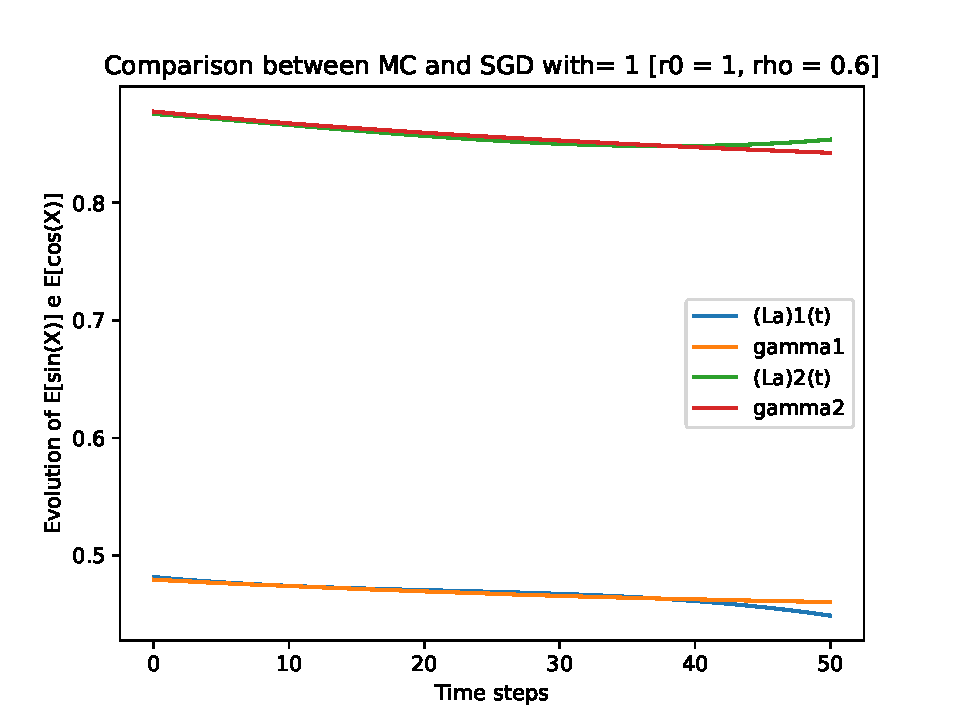
\includegraphics[width=0.9\textwidth]{images/graphics T = 0.5/n = 3, M = 1 sine and cosine.pdf}
\end{figure}
\begin{figure}[H]
\centering
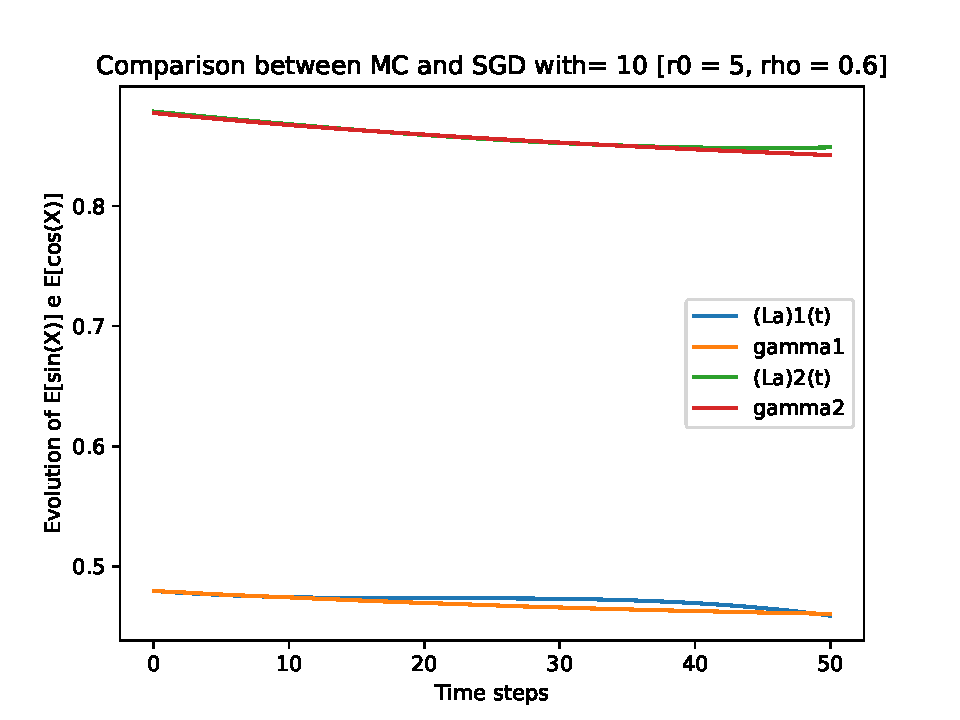
\includegraphics[width=0.9\textwidth]{images/graphics T = 0.5/n = 3, M = 10 sine and cosine.pdf}
\end{figure}
\begin{figure}[H]
\centering
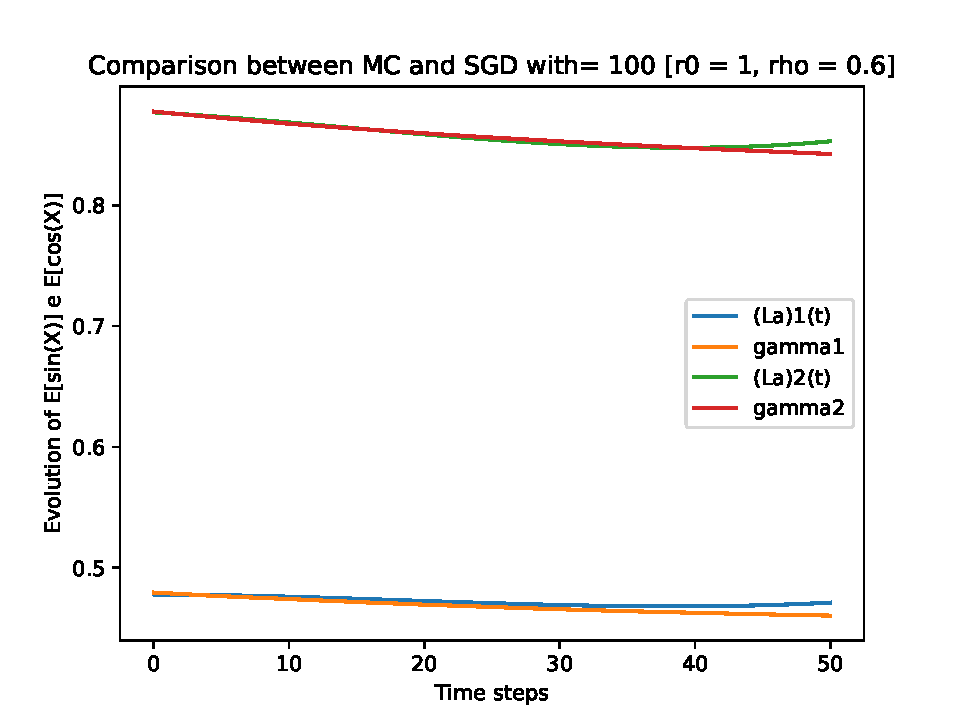
\includegraphics[width=0.9\textwidth]{images/graphics T = 0.5/n = 3, M = 100 sine and cosine.pdf}
\end{figure}
\begin{figure}[H]
\centering
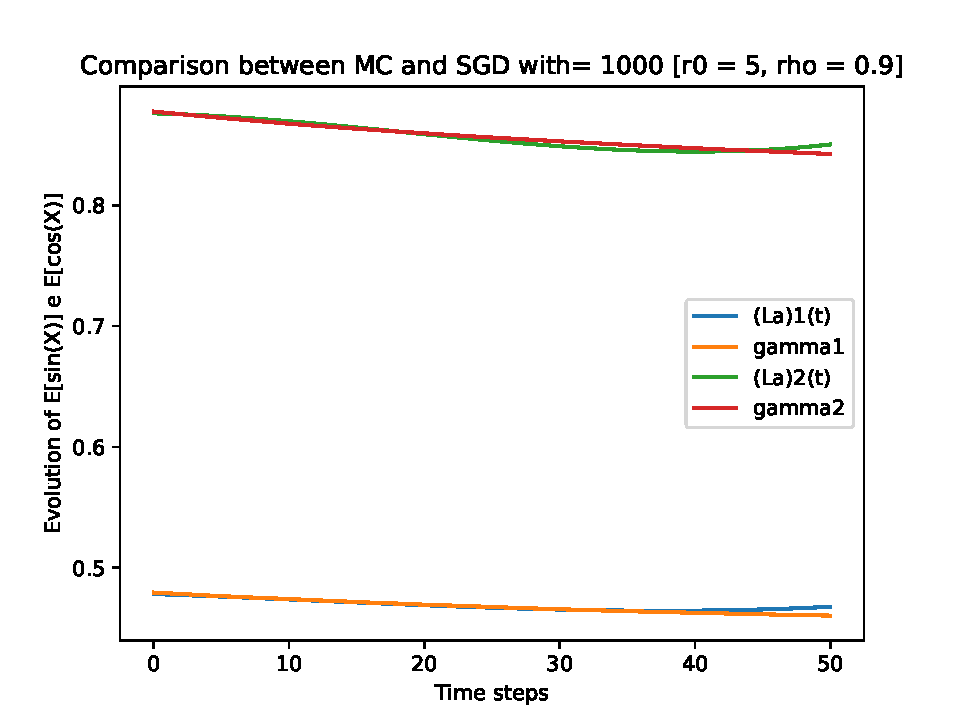
\includegraphics[width=0.9\textwidth]{images/graphics T = 0.5/n = 3, M = 1000 sine and cosine.pdf}
\end{figure}
\begin{figure}[H]
\centering
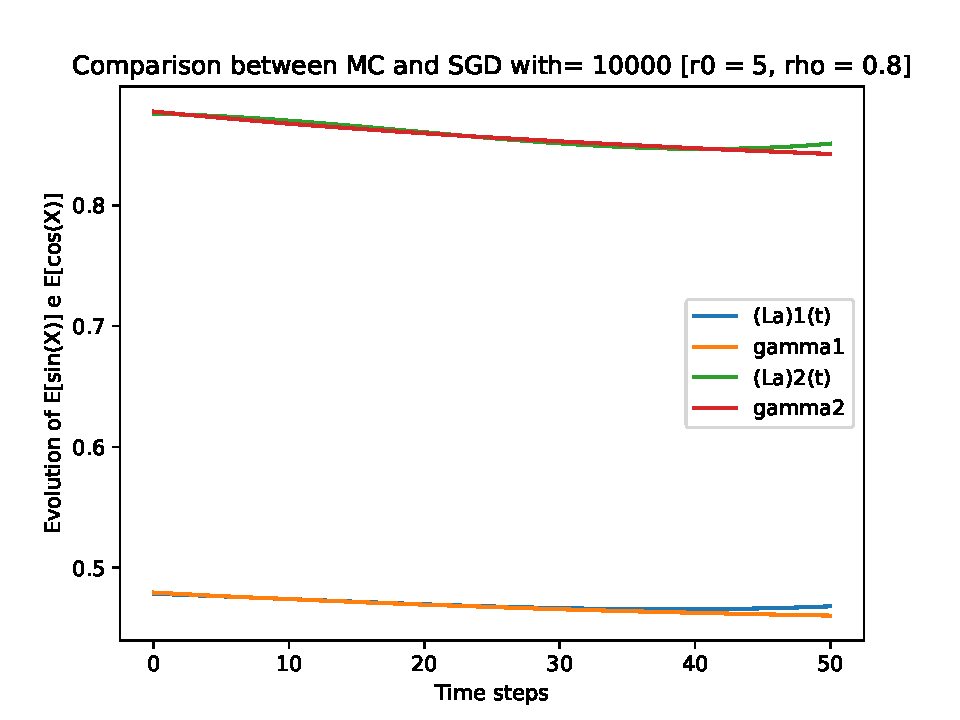
\includegraphics[width=0.9\textwidth]{images/graphics T = 0.5/n = 3, M = 10000 sine and cosine.pdf}
\end{figure}
\newpage
\section*{Caso n = 4}  
\begin{table}[H]
\centering
\addtolength{\leftskip}{-1.5cm}
\addtolength{\rightskip}{-1.5cm}
\begin{tabular}{|c|lll|}
\hline
$ $ & $r_0 = 1$ & $r_0 = 5$ & $r_0 = 10$ \\
\hline
$\rho = 0.6$ & 1.72 & 2.90 & 4.55 \\

$\rho = 0.7$ & 1.45 & 1.78 & 2.92 \\

$\rho = 0.8$ & 15.90 & 2.54 & 2.16 \\

$\rho = 0.9$ & 56.10 & 1.97 & 1.70 \\
\hline
\end{tabular}
\caption{Average execution
 times (in seconds $s$) with $M = 1$}
\end{table}
\begin{table}[H]
\centering
\addtolength{\leftskip}{-1.5cm}
\addtolength{\rightskip}{-1.5cm}
\begin{tabular}{|c|lllllllll|}
\hline
$ $ & $r_0 = 1$ & $r_0 = 1$ & $r_0 = 1$ & $r_0 = 5$ & $r_0 = 5$ & $r_0 = 5$ & $r_0 = 10$ & $r_0 = 10$ & $r_0 = 10$  \\
$ $ & min & max & average & min & max & average & min & max & average \\ 
\hline
$\rho = 0.6$ & 60 & 2080 & 484 & 270 & 1460 & 819 & 950 & 1680 & 1288 \\

$\rho = 0.7$ & 120 & 1350 & 412 & 150 & 850 & 505 & 350 & 1620 & 828\\

$\rho = 0.8$ & 120 & 22300 & 4501 & 250 & 1480 & 720 & 230 & 1510 & 609\\

$\rho = 0.9$ & 190 & 49999 & 15893.9 & 60 & 1520 & 560 & 210 & 1180 & 481\\
\hline
\end{tabular}
\caption{Number of iterations $m$ to achieve convergence with $M = 1$}
\end{table}
\begin{table}[H]
\centering
\addtolength{\leftskip}{-1.5cm}
\addtolength{\rightskip}{-1.5cm}
\begin{tabular}{|c|lll|}
\hline
$ $ & $r_0 = 1$ & $r_0 = 5$ & $r_0 = 10$ \\
\hline
$\rho = 0.6$ & 0.26 & 0.39 & 0.77 \\

$\rho = 0.7$ & 0.57 & 0.33 & 0.57 \\

$\rho = 0.8$ & 0.42 & 0.43 & 0.34 \\

$\rho = 0.9$ & 6.07 & 0.22 & 0.31 \\
\hline
\end{tabular}
\caption{Average execution
 times (in seconds $s$) with $M = 10$}
\end{table}
\begin{table}[H]
\centering
\addtolength{\leftskip}{-1.5cm}
\addtolength{\rightskip}{-1.5cm}
\begin{tabular}{|c|lllllllll|}
\hline
$ $ & $r_0 = 1$ & $r_0 = 1$ & $r_0 = 1$ & $r_0 = 5$ & $r_0 = 5$ & $r_0 = 5$ & $r_0 = 10$ & $r_0 = 10$ & $r_0 = 10$  \\
$ $ & min & max & average & min & max & average & min & max & average \\ 
\hline
$\rho = 0.6$ & 30 & 150 & 64 & 40 & 160 & 95 & 70 & 310 & 188\\

$\rho = 0.7$ & 30 & 450 & 139 & 20 & 150 & 80 & 40 & 220 & 140\\

$\rho = 0.8$ & 30 & 210 & 104 & 30 & 230 & 104 & 20 & 200 & 84\\

$\rho = 0.9$ & 20 & 6840 & 1486 & 10 & 120 & 54 & 30 & 180 & 76\\
\hline
\end{tabular}
\caption{Number of iterations $m$ to achieve convergence with $M = 10$}
\end{table}
\begin{table}[H]
\centering
\addtolength{\leftskip}{-1.5cm}
\addtolength{\rightskip}{-1.5cm}
\begin{tabular}{|c|lll|}
\hline
$ $ & $r_0 = 1$ & $r_0 = 5$ & $r_0 = 10$ \\
\hline
$\rho = 0.6$ & 0.16 & 0.12 & 0.23\\

$\rho = 0.7$ & 0.21 & 0.13 & 0.26 \\

$\rho = 0.8$ & 0.32 & 0.12 & 0.15 \\

$\rho = 0.9$ & 0.55 & 0.13 & 0.17 \\
\hline
\end{tabular}
\caption{Average execution
 times (in seconds $s$) with $M = 100$}
\end{table}
\begin{table}[H]
\centering
\addtolength{\leftskip}{-1.5cm}
\addtolength{\rightskip}{-1.5cm}
\begin{tabular}{|c|lllllllll|}
\hline
$ $ & $r_0 = 1$ & $r_0 = 1$ & $r_0 = 1$ & $r_0 = 5$ & $r_0 = 5$ & $r_0 = 5$ & $r_0 = 10$ & $r_0 = 10$ & $r_0 = 10$  \\
$ $ & min & max & average & min & max & average & min & max & average \\ 
\hline
$\rho = 0.6$ & 20 & 40 & 24 & 10 & 30 & 18 & 10 & 80 & 34\\

$\rho = 0.7$ & 20 & 90 & 31 & 10 & 50 & 19 & 20 & 100 & 38\\

$\rho = 0.8$ & 20 & 100 & 48 & 10 & 30 & 17 & 10 & 30 & 21\\

$\rho = 0.9$ & 40 & 180 & 82 & 10 & 30 & 20 & 10 & 40 & 25\\
\hline
\end{tabular}
\caption{Number of iterations $m$ to achieve convergence with $M = 100$}
\end{table}
\begin{table}[H]
\centering
\addtolength{\leftskip}{-1.5cm}
\addtolength{\rightskip}{-1.5cm}
\begin{tabular}{|c|lll|}
\hline
$ $ & $r_0 = 1$ & $r_0 = 5$ & $r_0 = 10$ \\
\hline
$\rho = 0.6$ & 0.56 & 0.13 & 0.2 \\

$\rho = 0.7$ & 0.66 & 0.13 & 0.20 \\

$\rho = 0.8$ & 0.99 & 0.14 & 0.16 \\

$\rho = 0.9$ & 1.53 & 0.15 & 0.14 \\
\hline
\end{tabular}
\caption{Average execution
 times (in seconds $s$) with $M = 1000$}
\end{table}
\begin{table}[H]
\centering
\addtolength{\leftskip}{-1.5cm}
\addtolength{\rightskip}{-1.5cm}
\begin{tabular}{|c|lllllllll|}
\hline
$ $ & $r_0 = 1$ & $r_0 = 1$ & $r_0 = 1$ & $r_0 = 5$ & $r_0 = 5$ & $r_0 = 5$ & $r_0 = 10$ & $r_0 = 10$ & $r_0 = 10$  \\
$ $ & min & max & average & min & max & average & min & max & average \\ 
\hline
$\rho = 0.6$ & 10 & 19 & 13.1 & 2 & 7 & 2.9 & 4 & 6 & 4.6\\

$\rho = 0.7$ & 13 & 20 & 15.4 & 2 & 5 & 2.9 & 4 & 6 & 4.6\\

$\rho = 0.8$ & 19 & 37 & 23.3 & 2 & 11 & 3.2 & 3 & 4 & 3.8\\

$\rho = 0.9$ & 30 & 44 & 35.9 & 2 & 16 & 3.6 & 3 & 4 & 3.3\\
\hline
\end{tabular}
\caption{Number of iterations $m$ to achieve convergence with $M = 1000$}
\end{table}
\begin{table}[H]
\centering
\addtolength{\leftskip}{-1.5cm}
\addtolength{\rightskip}{-1.5cm}
\begin{tabular}{|c|lll|}
\hline
$ $ & $r_0 = 1$ & $r_0 = 5$ & $r_0 = 10$ \\
\hline
$\rho = 0.6$ & 6.26 & 1.07 & 2.12 \\

$\rho = 0.7$ & 7.68 & 1.07 & 2.14 \\

$\rho = 0.8$ & 10.63 & 1.06 & 1.71 \\

$\rho = 0.9$ & 17.56 & 1.06 & 1.66 \\
\hline
\end{tabular}
\caption{Average execution
 times (in seconds $s$) with $M = 10000$}
\end{table}
\begin{table}[H]
\centering
\addtolength{\leftskip}{-1.5cm}
\addtolength{\rightskip}{-1.5cm}
\begin{tabular}{|c|lllllllll|}
\hline
$ $ & $r_0 = 1$ & $r_0 = 1$ & $r_0 = 1$ & $r_0 = 5$ & $r_0 = 5$ & $r_0 = 5$ & $r_0 = 10$ & $r_0 = 10$ & $r_0 = 10$  \\
$ $ & min & max & average & min & max & average & min & max & average \\ 
\hline
$\rho = 0.6$ & 11 & 12 & 11.6 & 2 & 2 & 2 & 4 & 4 & 4\\

$\rho = 0.7$ & 14 & 15 & 14.3 & 2 & 2 & 2 & 4 & 4 & 4\\

$\rho = 0.8$ & 18 & 21 & 19.7 & 2 & 2 & 2 & 3 & 4 & 3.2\\

$\rho = 0.9$ & 29 & 35 & 32.7 & 2 & 2 & 2 & 3 & 4 & 3.1\\
\hline
\end{tabular}
\caption{Number of iterations $m$ to achieve convergence with $M = 10000$}
\end{table}
\begin{figure}[H]
\centering
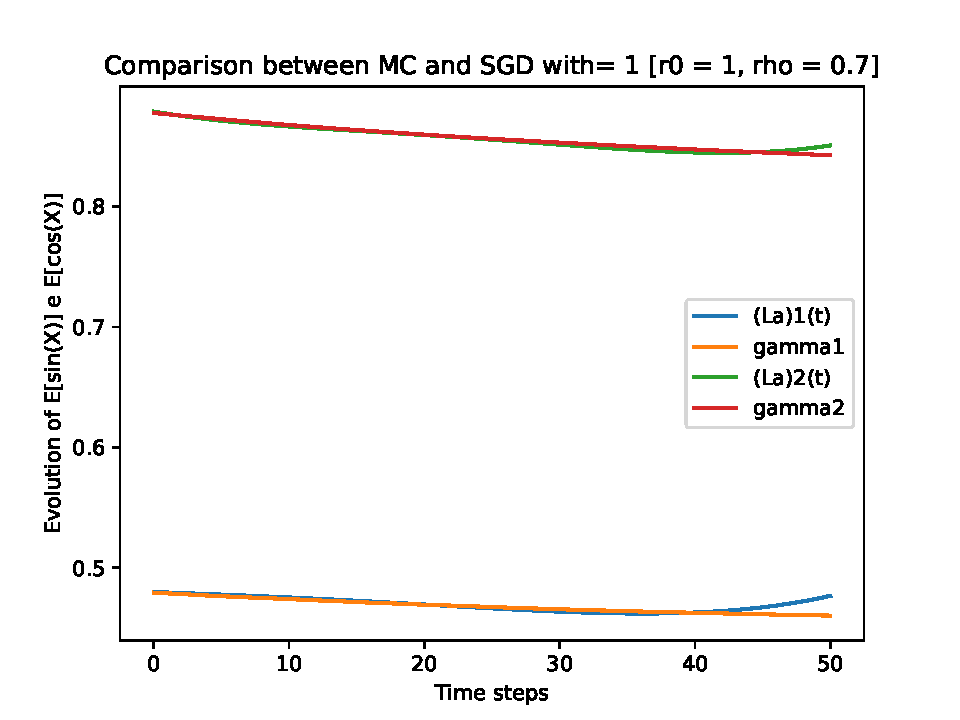
\includegraphics[width=0.9\textwidth]{images/graphics T = 0.5/n = 4, M = 1 sine and cosine.pdf}
\end{figure}
\begin{figure}[H]
\centering
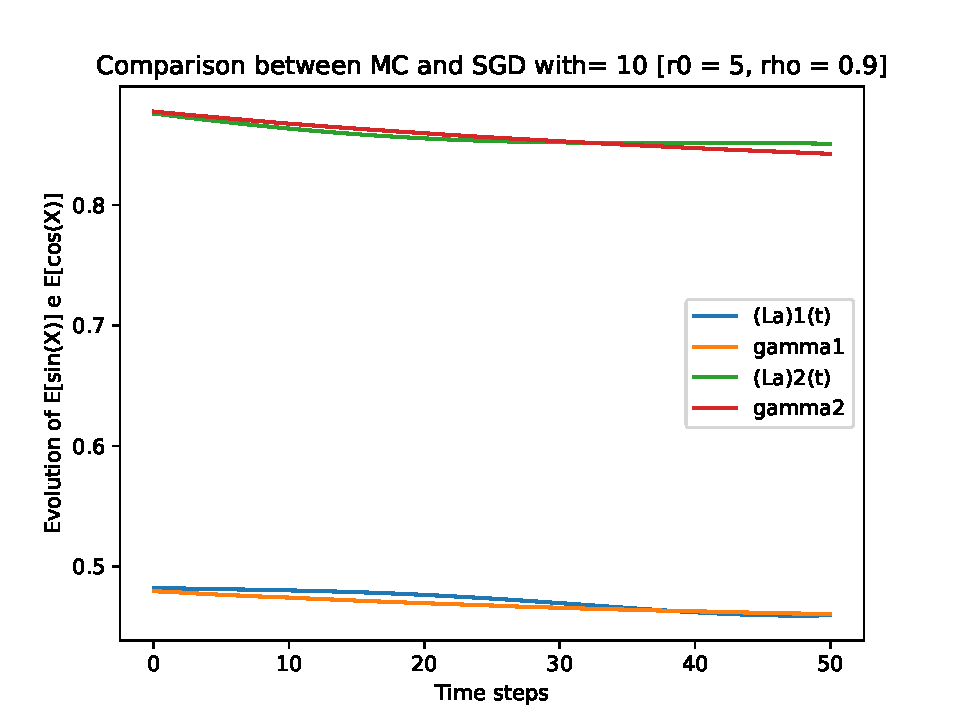
\includegraphics[width=0.9\textwidth]{images/graphics T = 0.5/n = 4, M = 10 sine and cosine.pdf}
\end{figure}
\begin{figure}[H]
\centering
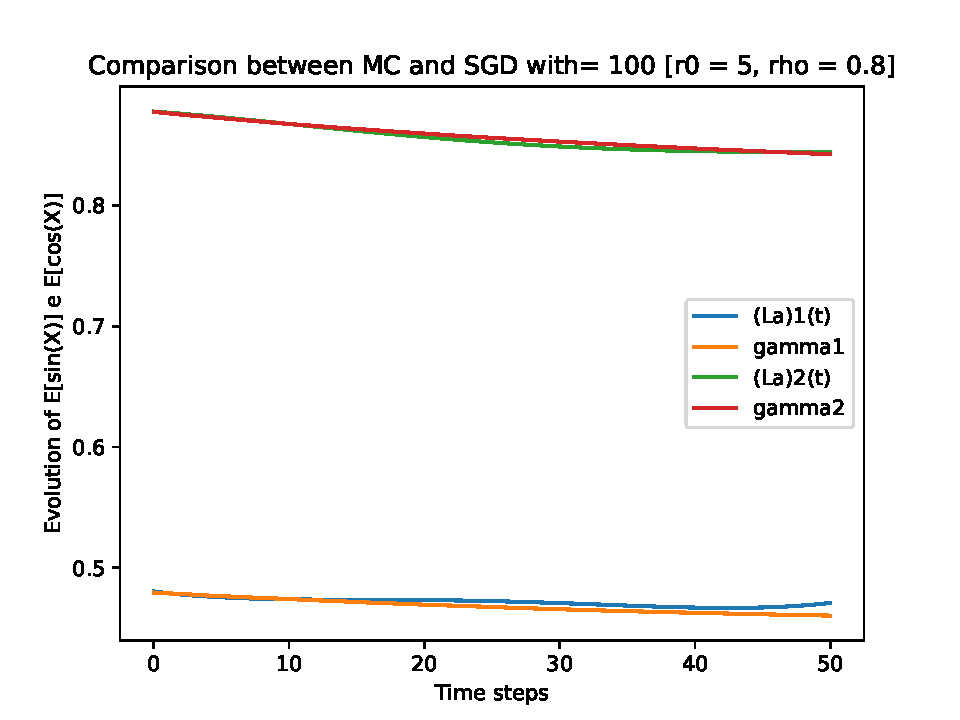
\includegraphics[width=0.9\textwidth]{images/graphics T = 0.5/n = 4, M = 100 sine and cosine.pdf}
\end{figure}
\begin{figure}[H]
\centering
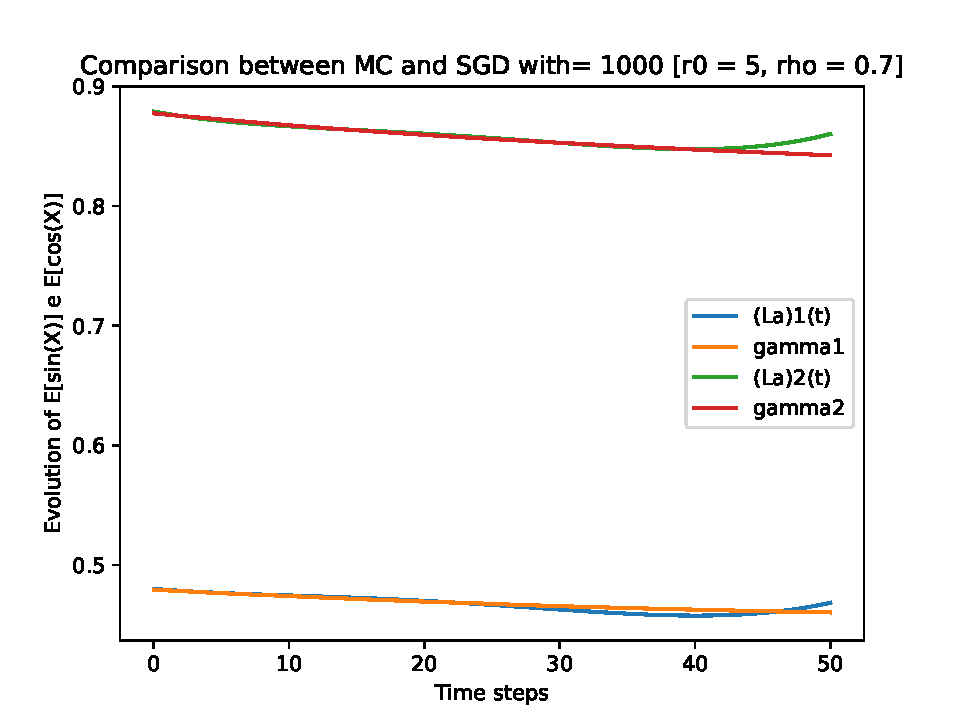
\includegraphics[width=0.9\textwidth]{images/graphics T = 0.5/n = 4, M = 1000 sine and cosine.pdf}
\end{figure}
\begin{figure}[H]
\centering
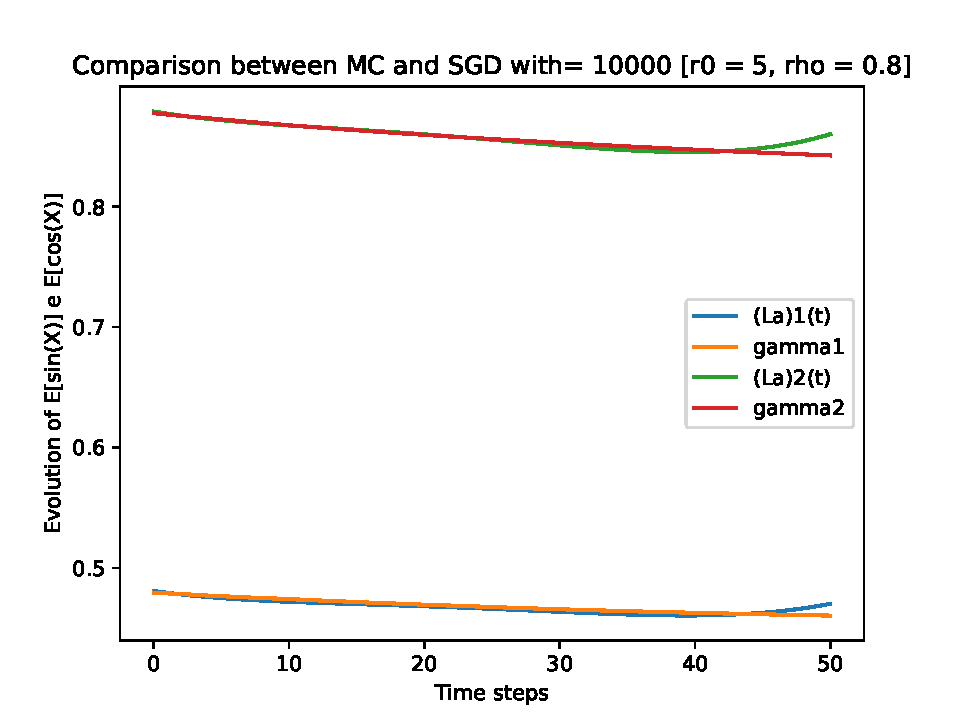
\includegraphics[width=0.9\textwidth]{images/graphics T = 0.5/n = 4, M = 10000 sine and cosine.pdf}
\end{figure}
\newpage
\section*{Caso n = 5} 
\begin{table}[H]
\centering
\addtolength{\leftskip}{-1.5cm}
\addtolength{\rightskip}{-1.5cm}
\begin{tabular}{|c|lll|}
\hline
$ $ & $r_0 = 1$ & $r_0 = 5$ & $r_0 = 10$ \\
\hline
$\rho = 0.6$ & 1.36 & 4.12 & 8.9 \\

$\rho = 0.7$ & 2.67 & 2.78 & 3.51 \\

$\rho = 0.8$ & 4.66 & 2.35 & 2.92 \\

$\rho = 0.9$ & 90.29 & 3.76 & 2.65 \\
\hline
\end{tabular}
\caption{Average execution
 times (in seconds $s$) with $M = 1$}
\end{table}
\begin{table}[H]
\centering
\addtolength{\leftskip}{-1.5cm}
\addtolength{\rightskip}{-1.5cm}
\begin{tabular}{|c|lllllllll|}
\hline
$ $ & $r_0 = 1$ & $r_0 = 1$ & $r_0 = 1$ & $r_0 = 5$ & $r_0 = 5$ & $r_0 = 5$ & $r_0 = 10$ & $r_0 = 10$ & $r_0 = 10$  \\
$ $ & min & max & average & min & max & average & min & max & average \\ 
\hline
$\rho = 0.6$ & 130 & 890 & 371 & 370 & 1760 & 866 & 610 & 2870 & 1714 \\

$\rho = 0.7$ & 110 & 2470 & 729 & 240 & 1070 & 589 & 420 & 1050 & 753\\

$\rho = 0.8$ & 90 & 4260 & 1271 & 130 & 1190 & 496 & 240 & 1100 & 613\\

$\rho = 0.9$ & 440 & 49999 & 22338.7 & 200 & 1330 & 661 & 160 & 1380 & 565\\
\hline
\end{tabular}
\caption{Number of iterations $m$ to achieve convergence with $M = 1$}
\end{table}
\begin{table}[H]
\centering
\addtolength{\leftskip}{-1.5cm}
\addtolength{\rightskip}{-1.5cm}
\begin{tabular}{|c|lll|}
\hline
$ $ & $r_0 = 1$ & $r_0 = 5$ & $r_0 = 10$ \\
\hline
$\rho = 0.6$ & 0.85 & 0.64 & 1.25 \\

$\rho = 0.7$ & 0.88 & 0.53 & 0.73 \\

$\rho = 0.8$ & 2.96 & 0.61 & 0.37 \\

$\rho = 0.9$ & 2.35 & 0.58 & 0.53 \\
\hline
\end{tabular}
\caption{Average execution
 times (in seconds $s$) with $M = 10$}
\end{table}
\begin{table}[H]
\centering
\addtolength{\leftskip}{-1.5cm}
\addtolength{\rightskip}{-1.5cm}
\begin{tabular}{|c|lllllllll|}
\hline
$ $ & $r_0 = 1$ & $r_0 = 1$ & $r_0 = 1$ & $r_0 = 5$ & $r_0 = 5$ & $r_0 = 5$ & $r_0 = 10$ & $r_0 = 10$ & $r_0 = 10$  \\
$ $ & min & max & average & min & max & average & min & max & average \\ 
\hline
$\rho = 0.6$ & 20 & 400 & 148 & 30 & 290 & 110 & 80 & 340 & 217\\

$\rho = 0.7$ & 20 & 630 & 157 & 20 & 190 & 89 & 40 & 250 & 132\\

$\rho = 0.8$ & 60 & 2110 & 513 & 20 & 280 & 104 & 30 & 100 & 68\\

$\rho = 0.9$ & 110 & 1210 & 411 & 30 & 250 & 103 & 20 & 210 & 93\\
\hline
\end{tabular}
\caption{Number of iterations $m$ to achieve convergence with $M = 10$}
\end{table}
\begin{table}[H]
\centering
\addtolength{\leftskip}{-1.5cm}
\addtolength{\rightskip}{-1.5cm}
\begin{tabular}{|c|lll|}
\hline
$ $ & $r_0 = 1$ & $r_0 = 5$ & $r_0 = 10$ \\
\hline
$\rho = 0.6$ & 0.29 & 0.28 & 0.25 \\

$\rho = 0.7$ & 0.48 & 0.25 & 0.40 \\

$\rho = 0.8$ & 0.98 & 0.18 & 0.38 \\

$\rho = 0.9$ & 1.31 & 0.29 & 0.19 \\
\hline
\end{tabular}
\caption{Average execution
 times (in seconds $s$) with $M = 100$}
\end{table}
\begin{table}[H]
\centering
\addtolength{\leftskip}{-1.5cm}
\addtolength{\rightskip}{-1.5cm}
\begin{tabular}{|c|lllllllll|}
\hline
$ $ & $r_0 = 1$ & $r_0 = 1$ & $r_0 = 1$ & $r_0 = 5$ & $r_0 = 5$ & $r_0 = 5$ & $r_0 = 10$ & $r_0 = 10$ & $r_0 = 10$  \\
$ $ & min & max & average & min & max & average & min & max & average \\ 
\hline
$\rho = 0.6$ & 20 & 40 & 27 & 10 & 60 & 21 & 10 & 40 & 22\\

$\rho = 0.7$ & 30 & 80 & 49 & 10 & 60 & 19 & 10 & 60 & 33\\

$\rho = 0.8$ & 40 & 180 & 85 & 10 & 30 & 16 & 10 & 50 & 30\\

$\rho = 0.9$ & 70 & 180 & 114 & 10 & 60 & 24 & 10 & 40 & 16\\
\hline
\end{tabular}
\caption{Number of iterations $m$ to achieve convergence with $M = 100$}
\end{table}
\begin{table}[H]
\centering
\addtolength{\leftskip}{-1.5cm}
\addtolength{\rightskip}{-1.5cm}
\begin{tabular}{|c|lll|}
\hline
$ $ & $r_0 = 1$ & $r_0 = 5$ & $r_0 = 10$ \\
\hline
$\rho = 0.6$ & 1.41 & 0.22 & 0.30 \\

$\rho = 0.7$ & 1.73 & 0.17 & 0.26 \\

$\rho = 0.8$ & 2.85 & 0.15 & 0.23 \\

$\rho = 0.9$ & 5.33 & 0.19 & 0.28 \\
\hline
\end{tabular}
\caption{Average execution
 times (in seconds $s$) with $M = 1000$}
\end{table}
\begin{table}[H]
\centering
\addtolength{\leftskip}{-1.5cm}
\addtolength{\rightskip}{-1.5cm}
\begin{tabular}{|c|lllllllll|}
\hline
$ $ & $r_0 = 1$ & $r_0 = 1$ & $r_0 = 1$ & $r_0 = 5$ & $r_0 = 5$ & $r_0 = 5$ & $r_0 = 10$ & $r_0 = 10$ & $r_0 = 10$  \\
$ $ & min & max & average & min & max & average & min & max & average \\ 
\hline
$\rho = 0.6$ & 15 & 25 & 18.6 & 1 & 8 & 2.6 & 3 & 6 & 3.8\\

$\rho = 0.7$ & 20 & 24 & 22.5 & 1 & 7 & 2.2 & 3 & 4 & 3.3\\

$\rho = 0.8$ & 32 & 45 & 37.5 & 1 & 4 & 1.9 & 3 & 4 & 3.2\\

$\rho = 0.9$ & 53 & 104 & 70.3 & 1 & 6 & 2.6 & 3 & 6 & 3.5\\
\hline
\end{tabular}
\caption{Number of iterations $m$ to achieve convergence with $M = 1000$}
\end{table}
\begin{table}[H]
\centering
\addtolength{\leftskip}{-1.5cm}
\addtolength{\rightskip}{-1.5cm}
\begin{tabular}{|c|lll|}
\hline
$ $ & $r_0 = 1$ & $r_0 = 5$ & $r_0 = 10$ \\
\hline
$\rho = 0.6$ & 16.95 & 1.42 & 3.38 \\

$\rho = 0.7$ & 23.12 & 1.48 & 3.20 \\

$\rho = 0.8$ & 36.69 & 1.3 & 3.22 \\

$\rho = 0.9$ & 68.4 & 1.13 & 3.13 \\
\hline
\end{tabular}
\caption{Average execution
 times (in seconds $s$) with $M = 10000$}
\end{table}
\begin{table}[H]
\centering
\addtolength{\leftskip}{-1.5cm}
\addtolength{\rightskip}{-1.5cm}
\begin{tabular}{|c|lllllllll|}
\hline
$ $ & $r_0 = 1$ & $r_0 = 1$ & $r_0 = 1$ & $r_0 = 5$ & $r_0 = 5$ & $r_0 = 5$ & $r_0 = 10$ & $r_0 = 10$ & $r_0 = 10$  \\
$ $ & min & max & average & min & max & average & min & max & average \\ 
\hline
$\rho = 0.6$ & 15 & 16 & 15.7 & 1 & 2 & 1.3 & 3 & 4 & 3.1\\

$\rho = 0.7$ & 21 & 23 & 21.5 & 1 & 2 & 1.4 & 3 & 3 & 3\\

$\rho = 0.8$ & 32 & 36 & 34.4 & 1 & 2 & 1.2 & 3 & 3 & 3\\

$\rho = 0.9$ & 59 & 66 & 63.4 & 1 & 1 & 1 & 2 & 3 & 2.9\\
\hline
\end{tabular}
\caption{Number of iterations $m$ to achieve convergence with $M = 10000$}
\end{table}
\begin{figure}[H]
\centering
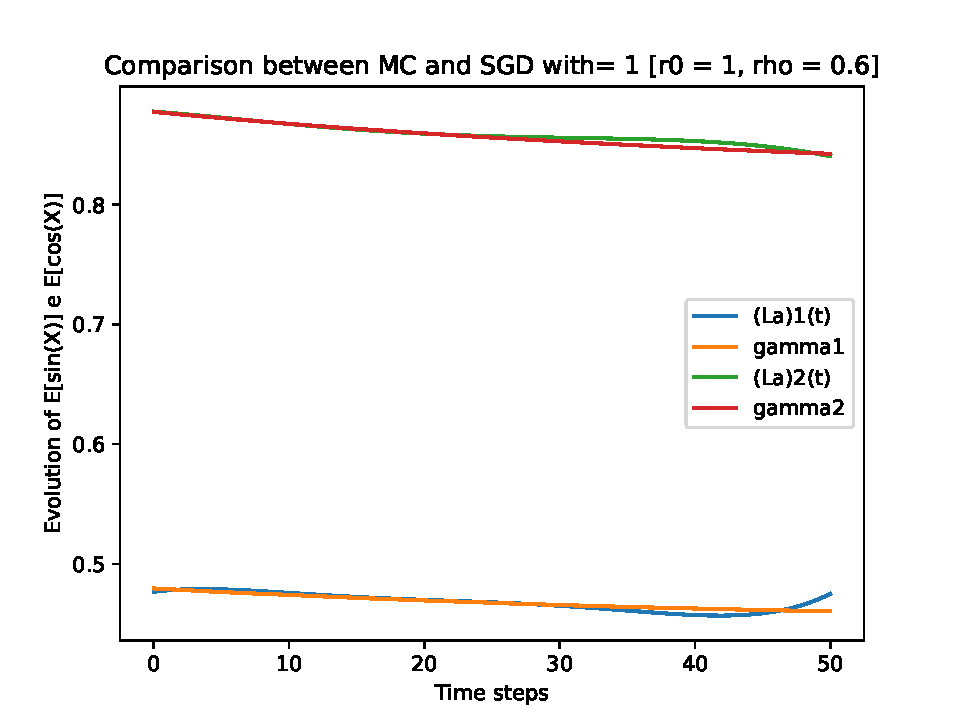
\includegraphics[width=0.9\textwidth]{images/graphics T = 0.5/n = 5, M = 1 sine and cosine.pdf}
\end{figure}
\begin{figure}[H]
\centering
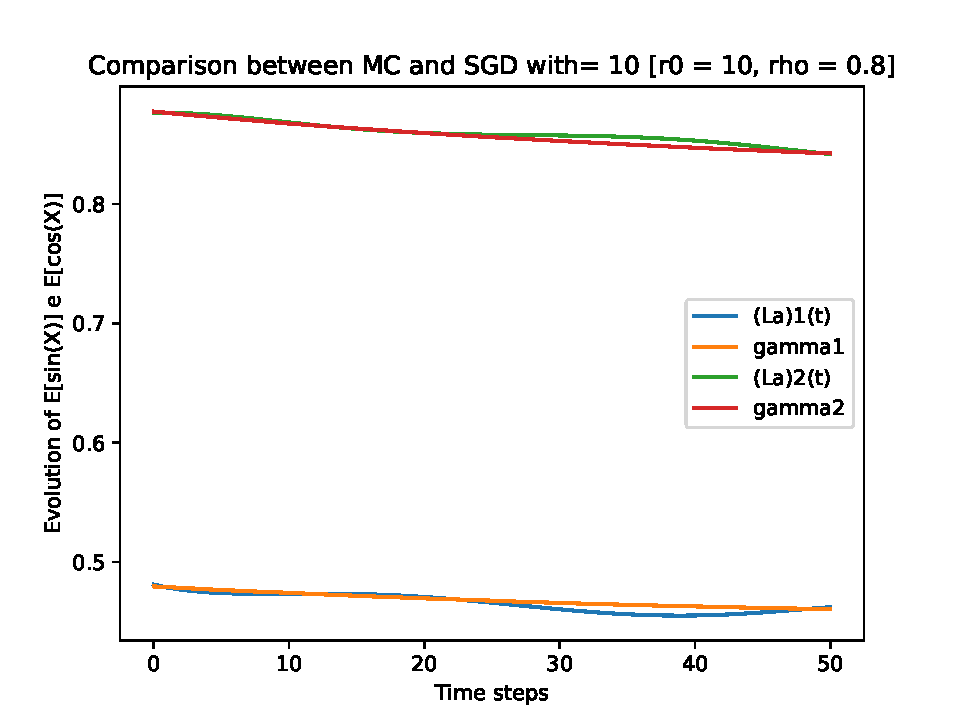
\includegraphics[width=0.9\textwidth]{images/graphics T = 0.5/n = 5, M = 10 sine and cosine.pdf}
\end{figure}
\begin{figure}[H]
\centering
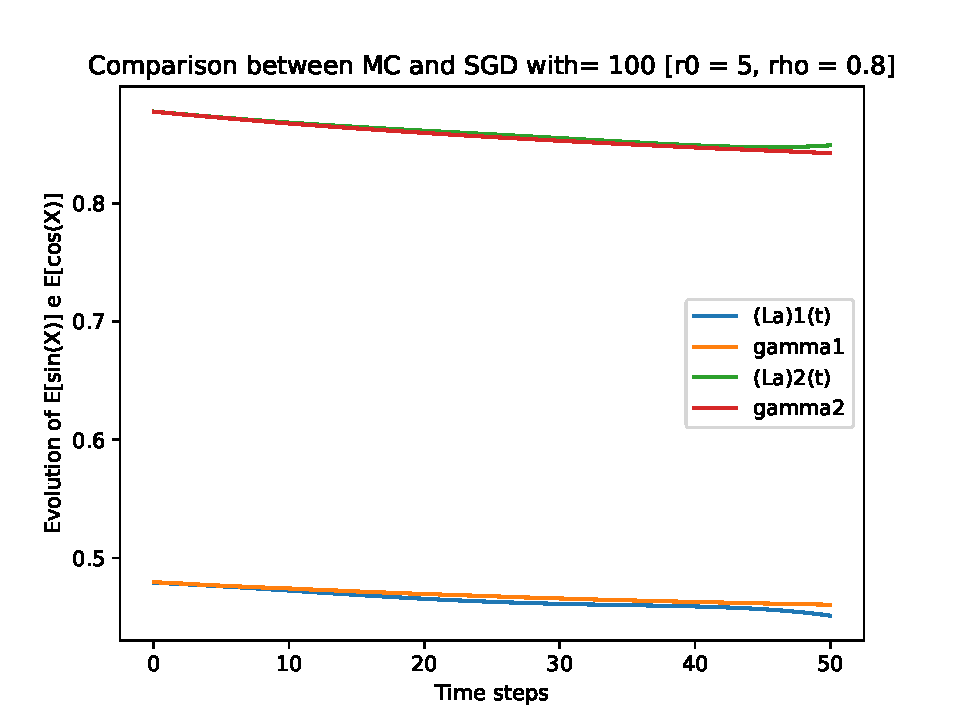
\includegraphics[width=0.9\textwidth]{images/graphics T = 0.5/n = 5, M = 100 sine and cosine.pdf}
\end{figure}
\begin{figure}[H]
\centering
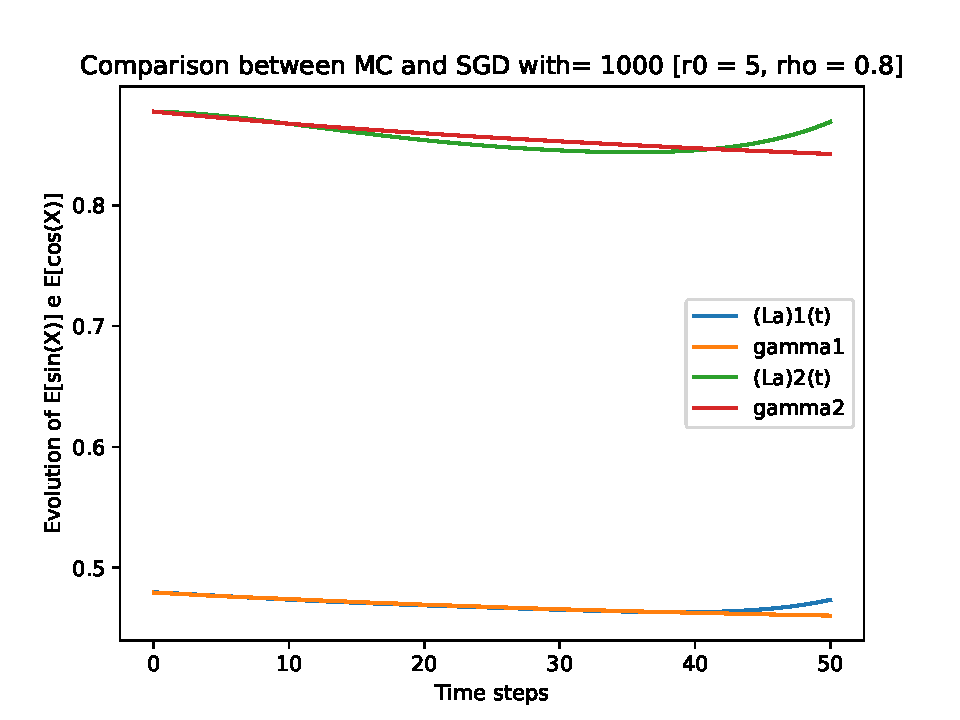
\includegraphics[width=0.9\textwidth]{images/graphics T = 0.5/n = 5, M = 1000 sine and cosine.pdf}
\end{figure}
\begin{figure}[H]
\centering
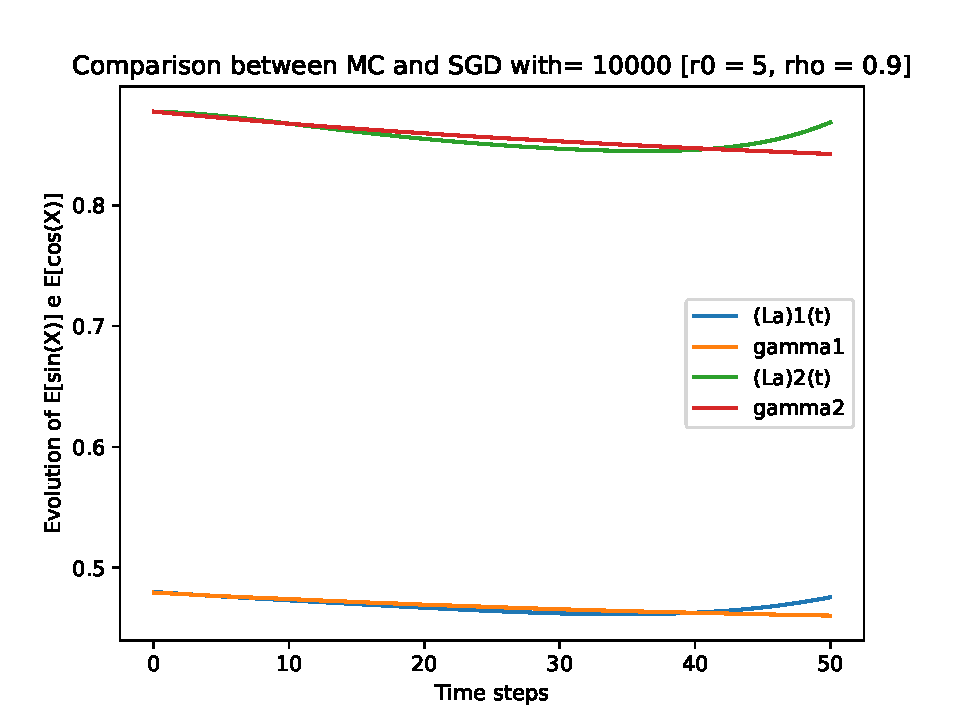
\includegraphics[width=0.9\textwidth]{images/graphics T = 0.5/n = 5, M = 10000 sine and cosine.pdf}
\end{figure}
\newpage
\section*{Caso n = 6}  
\begin{table}[H]
\centering
\addtolength{\leftskip}{-1.5cm}
\addtolength{\rightskip}{-1.5cm}
\begin{tabular}{|c|lll|}
\hline
$ $ & $r_0 = 1$ & $r_0 = 5$ & $r_0 = 10$ \\
\hline
$\rho = 0.6$ & 5.18 & 4.60 & 8.74 \\

$\rho = 0.7$ & 4.49 & 4.45 & 5.47 \\

$\rho = 0.8$ & 19.83 & 5.0 & 4.59 \\

$\rho = 0.9$ & 147.74 & 9.4 & 4.57 \\
\hline
\end{tabular}
\caption{Average execution
 times (in seconds $s$) with $M = 1$}
\end{table}
\begin{table}[H]
\centering
\addtolength{\leftskip}{-1.5cm}
\addtolength{\rightskip}{-1.5cm}
\begin{tabular}{|c|lllllllll|}
\hline
$ $ & $r_0 = 1$ & $r_0 = 1$ & $r_0 = 1$ & $r_0 = 5$ & $r_0 = 5$ & $r_0 = 5$ & $r_0 = 10$ & $r_0 = 10$ & $r_0 = 10$  \\
$ $ & min & max & average & min & max & average & min & max & average \\ 
\hline
$\rho = 0.6$ & 130 & 2650 & 864 & 260 & 1430 & 791 & 410 &  2140 & 1250 \\

$\rho = 0.7$ & 80 & 2080 & 731 & 210 & 1060 & 782 & 260 & 1370 & 766\\

$\rho = 0.8$ & 100 & 8230 & 3184 & 200 & 1550 & 809 & 260 & 1720 & 663\\

$\rho = 0.9$ & 180 & 49999 & 25371.6 & 220 & 6350 & 1360 & 190 & 2440 & 765\\
\hline
\end{tabular}
\caption{Number of iterations $m$ to achieve convergence with $M = 1$}
\end{table}
\begin{table}[H]
\centering
\addtolength{\leftskip}{-1.5cm}
\addtolength{\rightskip}{-1.5cm}
\begin{tabular}{|c|lll|}
\hline
$ $ & $r_0 = 1$ & $r_0 = 5$ & $r_0 = 10$ \\
\hline
$\rho = 0.6$ & 0.68 & 0.33 & 0.74 \\

$\rho = 0.7$ & 0.56 & 0.44 & 0.49 \\

$\rho = 0.8$ & 2.31 & 0.53 & 0.51 \\

$\rho = 0.9$ & 24.46 & 0.48 & 0.39 \\
\hline
\end{tabular}
\caption{Average execution
 times (in seconds $s$) with $M = 10$}
\end{table}
\begin{table}[H]
\centering
\addtolength{\leftskip}{-1.5cm}
\addtolength{\rightskip}{-1.5cm}
\begin{tabular}{|c|lllllllll|}
\hline
$ $ & $r_0 = 1$ & $r_0 = 1$ & $r_0 = 1$ & $r_0 = 5$ & $r_0 = 5$ & $r_0 = 5$ & $r_0 = 10$ & $r_0 = 10$ & $r_0 = 10$  \\
$ $ & min & max & average & min & max & average & min & max & average \\ 
\hline
$\rho = 0.6$ & 30 & 240 & 89 & 20 & 180 & 75 & 30 & 380 & 167\\

$\rho = 0.7$ & 40 & 160 & 77 & 40 & 210 & 99 & 40 & 160 & 110\\

$\rho = 0.8$ & 50 & 1080 & 329 & 40 & 300 & 119 & 40 & 290 & 116\\

$\rho = 0.9$ & 120 & 21270 & 4210 & 10 & 240 & 108 & 30 & 220 & 89\\
\hline
\end{tabular}
\caption{Number of iterations $m$ to achieve convergence with $M = 10$}
\end{table}
\begin{table}[H]
\centering
\addtolength{\leftskip}{-1.5cm}
\addtolength{\rightskip}{-1.5cm}
\begin{tabular}{|c|lll|}
\hline
$ $ & $r_0 = 1$ & $r_0 = 5$ & $r_0 = 10$ \\
\hline
$\rho = 0.6$ & 0.32 & 0.19 & 0.19 \\

$\rho = 0.7$ & 0.64 & 0.13 & 0.25 \\

$\rho = 0.8$ & 0.64 & 0.14 & 0.18 \\

$\rho = 0.9$ & 1.54 & 0.16 & 0.17 \\
\hline
\end{tabular}
\caption{Average execution
 times (in seconds $s$) with $M = 100$}
\end{table}
\begin{table}[H]
\centering
\addtolength{\leftskip}{-1.5cm}
\addtolength{\rightskip}{-1.5cm}
\begin{tabular}{|c|lllllllll|}
\hline
$ $ & $r_0 = 1$ & $r_0 = 1$ & $r_0 = 1$ & $r_0 = 5$ & $r_0 = 5$ & $r_0 = 5$ & $r_0 = 10$ & $r_0 = 10$ & $r_0 = 10$  \\
$ $ & min & max & average & min & max & average & min & max & average \\ 
\hline
$\rho = 0.6$ & 30 & 130 & 41 & 10 & 40 & 24 & 10 & 50 & 24\\

$\rho = 0.7$ & 40 & 290 & 81 & 10 & 30 & 16 & 10 & 60 & 31\\

$\rho = 0.8$ & 40 & 120 & 81 & 10 & 60 & 18 & 10 & 40 & 23\\

$\rho = 0.9$ & 110 & 300 & 196 & 10 & 60 & 20 & 10 & 40 & 22\\
\hline
\end{tabular}
\caption{Number of iterations $m$ to achieve convergence with $M = 100$}
\end{table}
\begin{table}[H]
\centering
\addtolength{\leftskip}{-1.5cm}
\addtolength{\rightskip}{-1.5cm}
\begin{tabular}{|c|lll|}
\hline
$ $ & $r_0 = 1$ & $r_0 = 5$ & $r_0 = 10$ \\
\hline
$\rho = 0.6$ & 1.28 & 0.13 & 0.20 \\

$\rho = 0.7$ & 1.87 & 0.12 & 0.19 \\

$\rho = 0.8$ & 2.90 & 0.16 & 0.13 \\

$\rho = 0.9$ & 6.89 & 0.11 & 0.16 \\
\hline
\end{tabular}
\caption{Average execution
 times (in seconds $s$) with $M = 1000$}
\end{table}
\begin{table}[H]
\centering
\addtolength{\leftskip}{-1.5cm}
\addtolength{\rightskip}{-1.5cm}
\begin{tabular}{|c|lllllllll|}
\hline
$ $ & $r_0 = 1$ & $r_0 = 1$ & $r_0 = 1$ & $r_0 = 5$ & $r_0 = 5$ & $r_0 = 5$ & $r_0 = 10$ & $r_0 = 10$ & $r_0 = 10$  \\
$ $ & min & max & average & min & max & average & min & max & average \\ 
\hline
$\rho = 0.6$ & 22 & 29 & 23.7 & 1 & 4 & 2.5 & 3 & 8 & 3.8\\

$\rho = 0.7$ & 31 & 43 & 34.6 & 1 & 4 & 2.1 & 2 & 7 & 3.5\\

$\rho = 0.8$ & 50 & 56 & 53.4 & 1 & 7 & 2.9 & 2 & 4 & 2.5\\

$\rho = 0.9$ & 105 & 174 & 127.3 & 1 & 6 & 2 & 2 & 4 & 2.9\\
\hline
\end{tabular}
\caption{Number of iterations $m$ to achieve convergence with $M = 1000$}
\end{table}
\begin{table}[H]
\centering
\addtolength{\leftskip}{-1.5cm}
\addtolength{\rightskip}{-1.5cm}
\begin{tabular}{|c|lll|}
\hline
$ $ & $r_0 = 1$ & $r_0 = 5$ & $r_0 = 10$ \\
\hline
$\rho = 0.6$ & 16.77 & 0.77 & 1.92 \\

$\rho = 0.7$ & 24.63 & 1.00 & 1.61 \\

$\rho = 0.8$ & 41.76 & 0.77 & 1.61 \\

$\rho = 0.9$ & 93.11 & 0.85 & 1.54 \\
\hline
\end{tabular}
\caption{Average execution
 times (in seconds $s$) with $M = 10000$}
\end{table}
\begin{table}[H]
\centering
\addtolength{\leftskip}{-1.5cm}
\addtolength{\rightskip}{-1.5cm}
\begin{tabular}{|c|lllllllll|}
\hline
$ $ & $r_0 = 1$ & $r_0 = 1$ & $r_0 = 1$ & $r_0 = 5$ & $r_0 = 5$ & $r_0 = 5$ & $r_0 = 10$ & $r_0 = 10$ & $r_0 = 10$  \\
$ $ & min & max & average & min & max & average & min & max & average \\ 
\hline
$\rho = 0.6$ & 21 & 23 & 21.8 & 1 & 1 & 1 & 2 & 3 & 2.5\\

$\rho = 0.7$ & 31 & 34 & 31.9 & 1 & 2 & 1.3 & 2 & 3 & 2.1\\

$\rho = 0.8$ & 52 & 59 & 54.4 & 1 & 1 & 1 & 2 & 3 & 2.1\\

$\rho = 0.9$ & 114 & 128 & 121.3 & 1 & 2 & 1.1 & 2 & 2 & 2\\
\hline
\end{tabular}
\caption{Number of iterations $m$ to achieve convergence with $M = 10000$}
\end{table}
\begin{figure}[H]
\centering
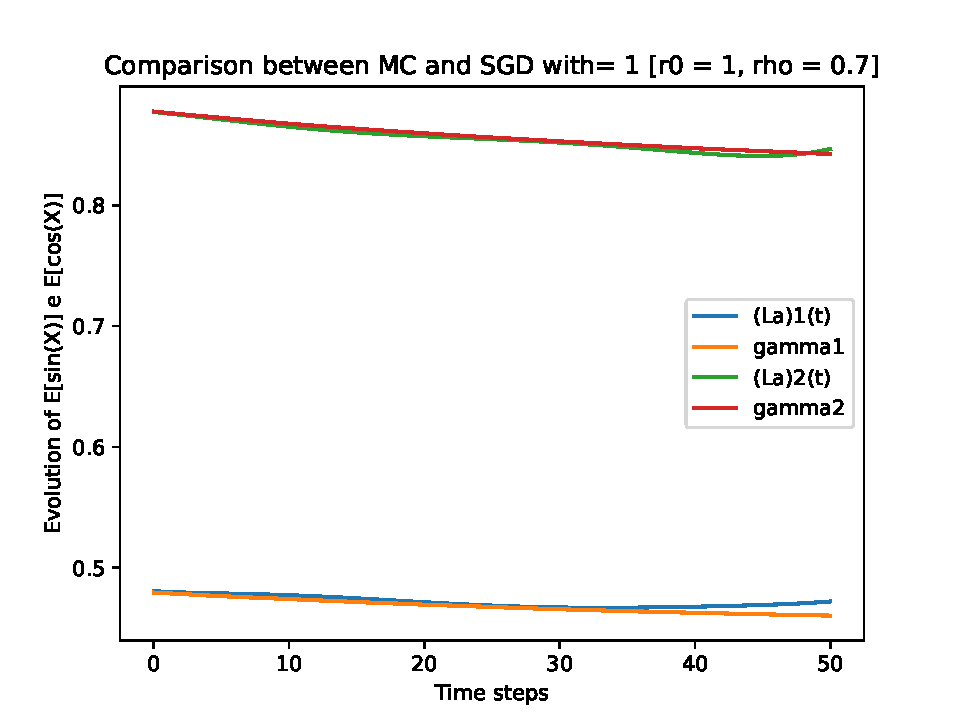
\includegraphics[width=0.9\textwidth]{images/graphics T = 0.5/n = 6, M = 1 sine and cosine.pdf}
\end{figure}
\begin{figure}[H]
\centering
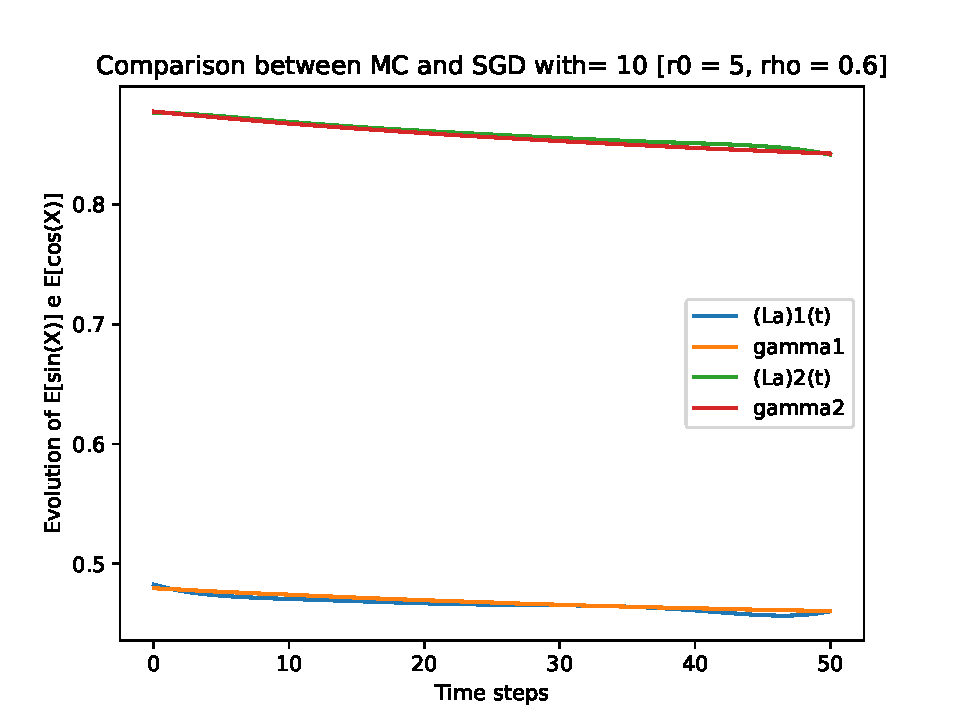
\includegraphics[width=0.9\textwidth]{images/graphics T = 0.5/n = 6, M = 10 sine and cosine.pdf}
\end{figure}
\begin{figure}[H]
\centering
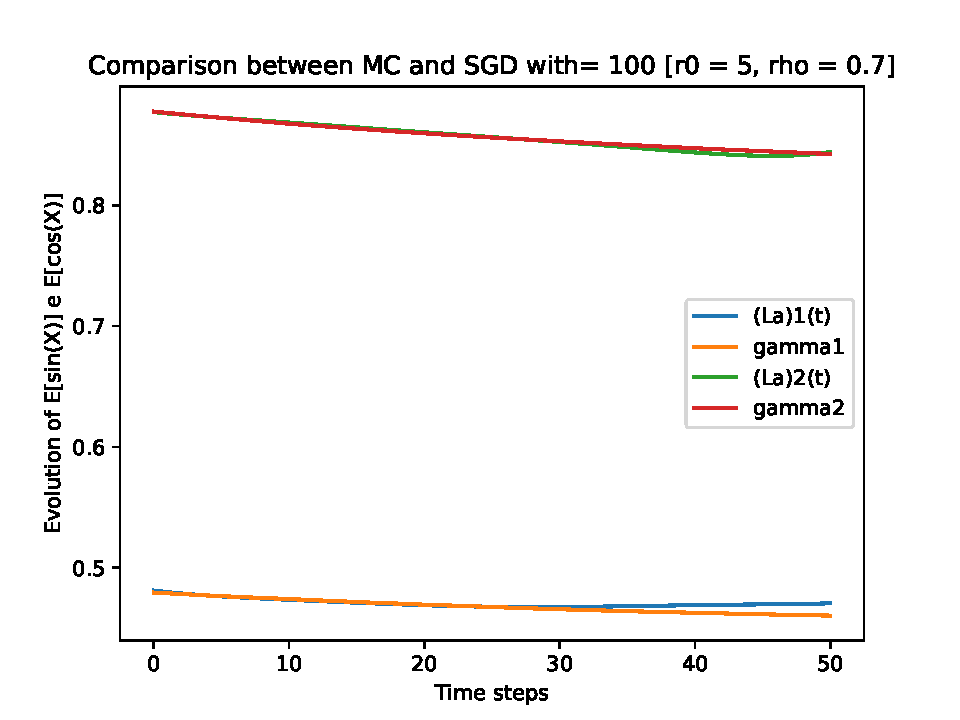
\includegraphics[width=0.9\textwidth]{images/graphics T = 0.5/n = 6, M = 100 sine and cosine.pdf}
\end{figure}
\begin{figure}[H]
\centering
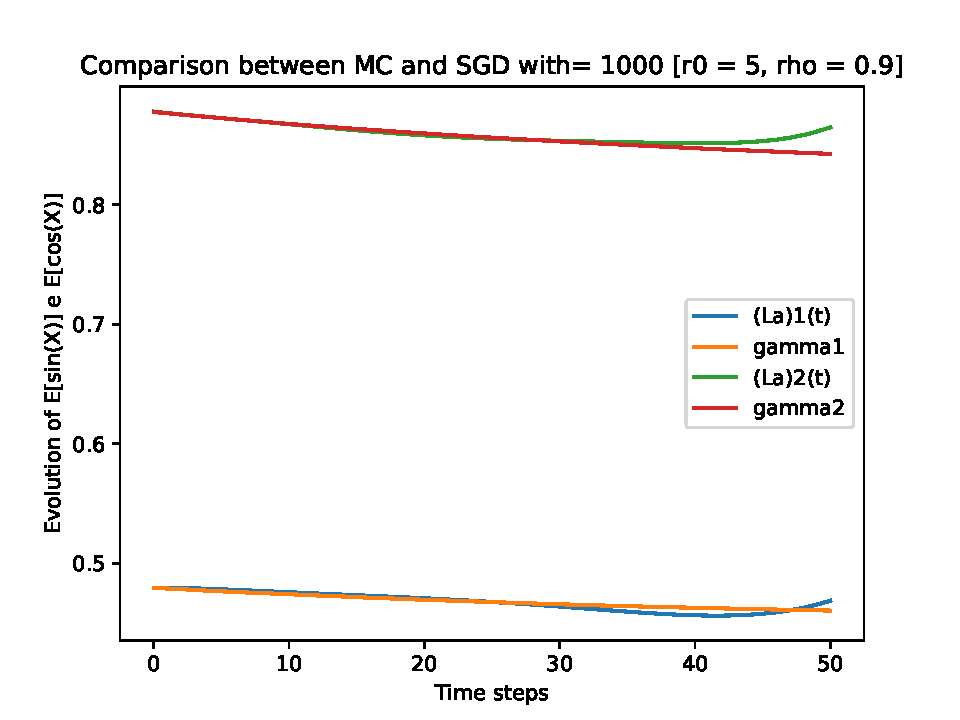
\includegraphics[width=0.9\textwidth]{images/graphics T = 0.5/n = 6, M = 1000 sine and cosine.pdf}
\end{figure}
\begin{figure}[H]
\centering
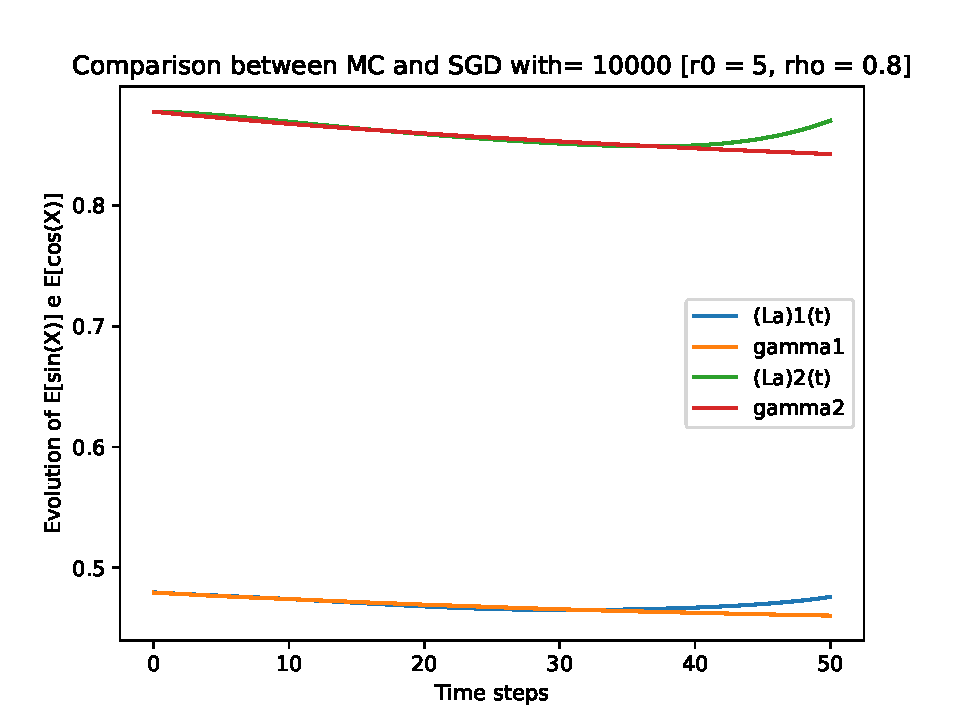
\includegraphics[width=0.9\textwidth]{images/graphics T = 0.5/n = 6, M = 10000 sine and cosine.pdf}
\end{figure}
\newpage
\section{T = 1}
\section*{Caso n = 3} 
\begin{table}[H]
\centering
\addtolength{\leftskip}{-1.5cm}
\addtolength{\rightskip}{-1.5cm}
\begin{tabular}{|c|lll|}
\hline
$ $ & $r_0 = 1$ & $r_0 = 5$ & $r_0 = 10$ \\
\hline
$\rho = 0.6$ & 4.60 & 14.19 & 30.59 \\

$\rho = 0.7$ & 6.06 & 8.29 & 13.83 \\

$\rho = 0.8$ & 17.74 & 6.40 & 9.32 \\

$\rho = 0.9$ & 29.5 & 5.47 & 5.58 \\
\hline
\end{tabular}
\caption{Average execution
 times (in seconds $s$) with $M = 1$}
\end{table}
\begin{table}[H]
\centering
\addtolength{\leftskip}{-1.5cm}
\addtolength{\rightskip}{-1.5cm}
\begin{tabular}{|c|lllllllll|}
\hline
$ $ & $r_0 = 1$ & $r_0 = 1$ & $r_0 = 1$ & $r_0 = 5$ & $r_0 = 5$ & $r_0 = 5$ & $r_0 = 10$ & $r_0 = 10$ & $r_0 = 10$  \\
$ $ & min & max & average & min & max & average & min & max & average \\ 
\hline
$\rho = 0.6$ & 220 & 1470 & 683 & 1090 & 3170 & 2090 & 2110 & 6360 & 4544 \\

$\rho = 0.7$ & 170 & 2540 & 921 & 280 & 2290 & 1199 & 890 & 4200 & 2029\\

$\rho = 0.8$ & 160 & 13840 & 2754 & 390 & 1590 & 947 & 580 & 2140 & 1350\\

$\rho = 0.9$ & 690 & 10410 & 4305 & 330 & 1740 & 812 & 230 & 1860 & 836\\
\hline
\end{tabular}
\caption{Number of iterations $m$ to achieve convergence with $M = 1$}
\end{table}
\begin{table}[H]
\centering
\addtolength{\leftskip}{-1.5cm}
\addtolength{\rightskip}{-1.5cm}
\begin{tabular}{|c|lll|}
\hline
$ $ & $r_0 = 1$ & $r_0 = 5$ & $r_0 = 10$ \\
\hline
$\rho = 0.6$ & 1.22 & 1.81 & 3.94 \\

$\rho = 0.7$ & 1.23 & 1.34 & 2.58 \\

$\rho = 0.8$ & 2.29 & 1.33 & 1.53 \\

$\rho = 0.9$ & 6.92 & 0.93 & 1.95 \\
\hline
\end{tabular}
\caption{Average execution
 times (in seconds $s$) with $M = 10$}
\end{table}
\begin{table}[H]
\centering
\addtolength{\leftskip}{-1.5cm}
\addtolength{\rightskip}{-1.5cm}
\begin{tabular}{|c|lllllllll|}
\hline
$ $ & $r_0 = 1$ & $r_0 = 1$ & $r_0 = 1$ & $r_0 = 5$ & $r_0 = 5$ & $r_0 = 5$ & $r_0 = 10$ & $r_0 = 10$ & $r_0 = 10$  \\
$ $ & min & max & average & min & max & average & min & max & average \\ 
\hline
$\rho = 0.6$ & 50 & 330 & 159 & 90 & 440 & 234 & 200 & 1060 & 496 \\

$\rho = 0.7$ & 10 & 500 & 160 & 70 & 500 & 173 & 140 & 500 & 323\\

$\rho = 0.8$ & 30 & 1210 & 298 & 50 & 480 & 172 & 110 & 410 & 194\\

$\rho = 0.9$ & 50 & 2210 & 904 & 50 & 290 & 120 & 20 & 550 & 253\\
\hline
\end{tabular}
\caption{Number of iterations $m$ to achieve convergence with $M = 10$}
\end{table}
\begin{table}[H]
\centering
\addtolength{\leftskip}{-1.5cm}
\addtolength{\rightskip}{-1.5cm}
\begin{tabular}{|c|lll|}
\hline
$ $ & $r_0 = 1$ & $r_0 = 5$ & $r_0 = 10$ \\
\hline
$\rho = 0.6$ & 0.27 & 0.68 & 0.88 \\

$\rho = 0.7$ & 0.39 & 0.47 & 0.92 \\

$\rho = 0.8$ & 0.32 & 0.45 & 0.47 \\

$\rho = 0.9$ & 0.37 & 0.59 &  0.59 \\
\hline
\end{tabular}
\caption{Average execution
 times (in seconds $s$) with $M = 100$}
\end{table}
\begin{table}[H]
\centering
\addtolength{\leftskip}{-1.5cm}
\addtolength{\rightskip}{-1.5cm}
\begin{tabular}{|c|lllllllll|}
\hline
$ $ & $r_0 = 1$ & $r_0 = 1$ & $r_0 = 1$ & $r_0 = 5$ & $r_0 = 5$ & $r_0 = 5$ & $r_0 = 10$ & $r_0 = 10$ & $r_0 = 10$  \\
$ $ & min & max & average & min & max & average & min & max & average \\ 
\hline
$\rho = 0.6$ & 10 & 40 & 21 & 10 & 100 & 54 & 40 & 130 & 69 \\

$\rho = 0.7$ & 10 & 50 & 30 & 10 & 70 & 38 & 20 & 110 & 74\\

$\rho = 0.8$ & 10 & 40 & 25 & 20 & 70 & 36 & 20 & 90 & 38\\

$\rho = 0.9$ & 10 & 50 & 29 & 20 & 150 & 46 & 30 & 90 & 47\\
\hline
\end{tabular}
\caption{Number of iterations $m$ to achieve convergence with $M = 100$}
\end{table}
\begin{table}[H]
\centering
\addtolength{\leftskip}{-1.5cm}
\addtolength{\rightskip}{-1.5cm}
\begin{tabular}{|c|lll|}
\hline
$ $ & $r_0 = 1$ & $r_0 = 5$ & $r_0 = 10$ \\
\hline
$\rho = 0.6$ & 0.49 & 0.62 & 1.82 \\

$\rho = 0.7$ & 0.75 & 0.54 & 1.21 \\

$\rho = 0.8$ & 0.66 & 0.44 & 1.03 \\

$\rho = 0.9$ & 0.82 & 0.46 & 0.75 \\
\hline
\end{tabular}
\caption{Average execution
 times (in seconds $s$) with $M = 1000$}
\end{table}
\begin{table}[H]
\centering
\addtolength{\leftskip}{-1.5cm}
\addtolength{\rightskip}{-1.5cm}
\begin{tabular}{|c|lllllllll|}
\hline
$ $ & $r_0 = 1$ & $r_0 = 1$ & $r_0 = 1$ & $r_0 = 5$ & $r_0 = 5$ & $r_0 = 5$ & $r_0 = 10$ & $r_0 = 10$ & $r_0 = 10$  \\
$ $ & min & max & average & min & max & average & min & max & average \\ 
\hline
$\rho = 0.6$ & 5 & 7 & 5.6 & 6 & 12 & 6.9 & 19 & 24 & 20.8 \\

$\rho = 0.7$ & 5 & 27 & 8.9 & 5 & 9 & 6.3 & 13 & 16 & 14.4 \\

$\rho = 0.8$ & 6 & 10 & 7.9 & 4 & 10 & 5.1 & 10 & 14 & 11.8 \\

$\rho = 0.9$ & 7 & 18 & 9.7 & 4 & 13 & 5.4 & 8 & 13 & 8.9\\
\hline
\end{tabular}
\caption{Number of iterations $m$ to achieve convergence with $M = 1000$}
\end{table}
\begin{table}[H]
\centering
\addtolength{\leftskip}{-1.5cm}
\addtolength{\rightskip}{-1.5cm}
\begin{tabular}{|c|lll|}
\hline
$ $ & $r_0 = 1$ & $r_0 = 5$ & $r_0 = 10$ \\
\hline
$\rho = 0.6$ & 4.71 & 5.83 & 18.25 \\

$\rho = 0.7$ & 5.65 & 4.93 & 12.90 \\

$\rho = 0.8$ & 6.19 & 3.93 & 9.96 \\

$\rho = 0.9$ & 7.45 & 3.98 & 7.93 \\
\hline
\end{tabular}
\caption{Average execution
 times (in seconds $s$) with $M = 10000$}
\end{table}
\begin{table}[H]
\centering
\addtolength{\leftskip}{-1.5cm}
\addtolength{\rightskip}{-1.5cm}
\begin{tabular}{|c|lllllllll|}
\hline
$ $ & $r_0 = 1$ & $r_0 = 1$ & $r_0 = 1$ & $r_0 = 5$ & $r_0 = 5$ & $r_0 = 5$ & $r_0 = 10$ & $r_0 = 10$ & $r_0 = 10$  \\
$ $ & min & max & average & min & max & average & min & max & average \\ 
\hline
$\rho = 0.6$ & 4 & 5 & 4.8 & 6 & 6 & 6 & 17 & 20 & 17.8 \\

$\rho = 0.7$ & 5 & 7 & 5.5 & 5 & 5 & 5 & 13 & 13 & 13\\

$\rho = 0.8$ & 6 & 7 & 6.1 & 4 & 4 & 4 & 10 & 10 & 10\\

$\rho = 0.9$ & 7 & 11 & 7.7 & 4 & 4 & 4 & 8 & 8 & 8\\
\hline
\end{tabular}
\caption{Number of iterations $m$ to achieve convergence with $M = 10000$}
\end{table}
\begin{figure}[H]
\centering
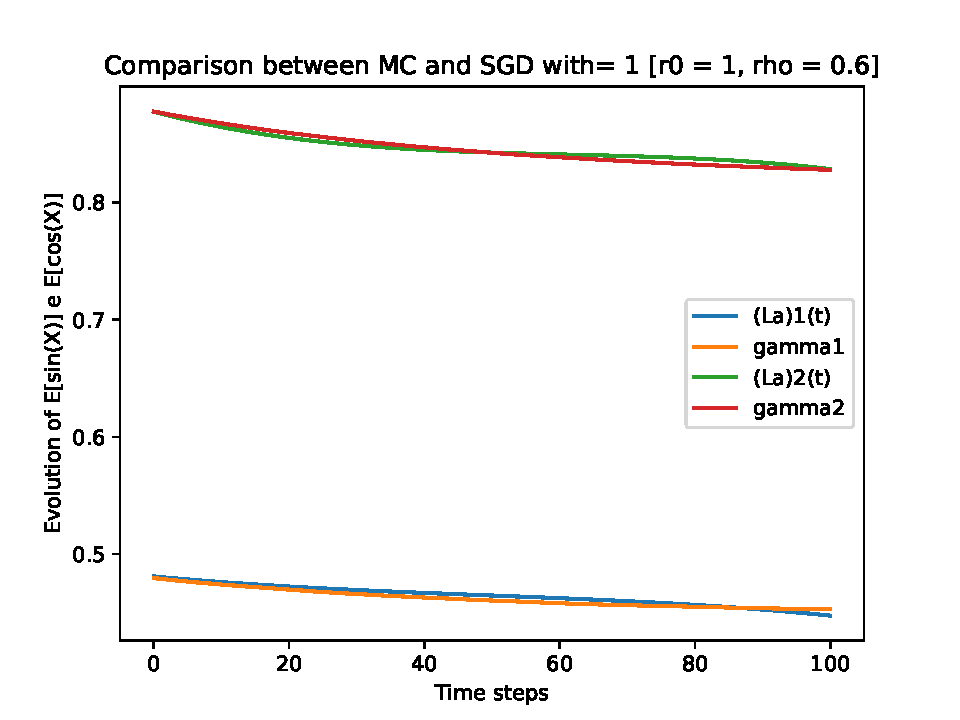
\includegraphics[width=0.9\textwidth]{images/graphics T = 1/n = 3, M = 1 sine and cosine.pdf}
\end{figure}
\begin{figure}[H]
\centering
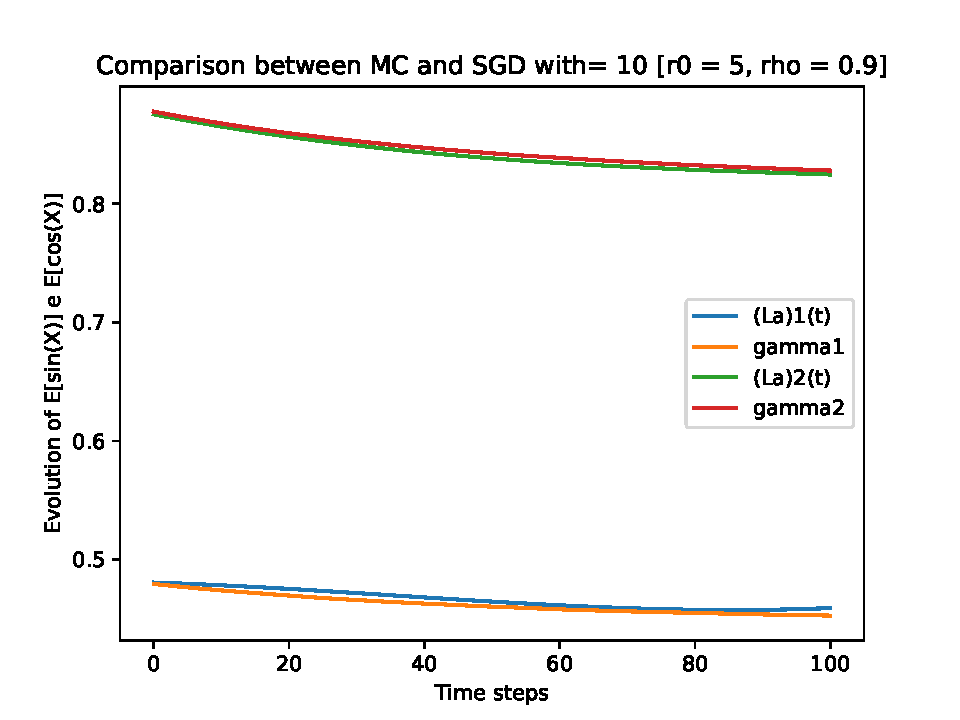
\includegraphics[width=0.9\textwidth]{images/graphics T = 1/n = 3, M = 10 sine and cosine.pdf}
\end{figure}
\begin{figure}[H]
\centering
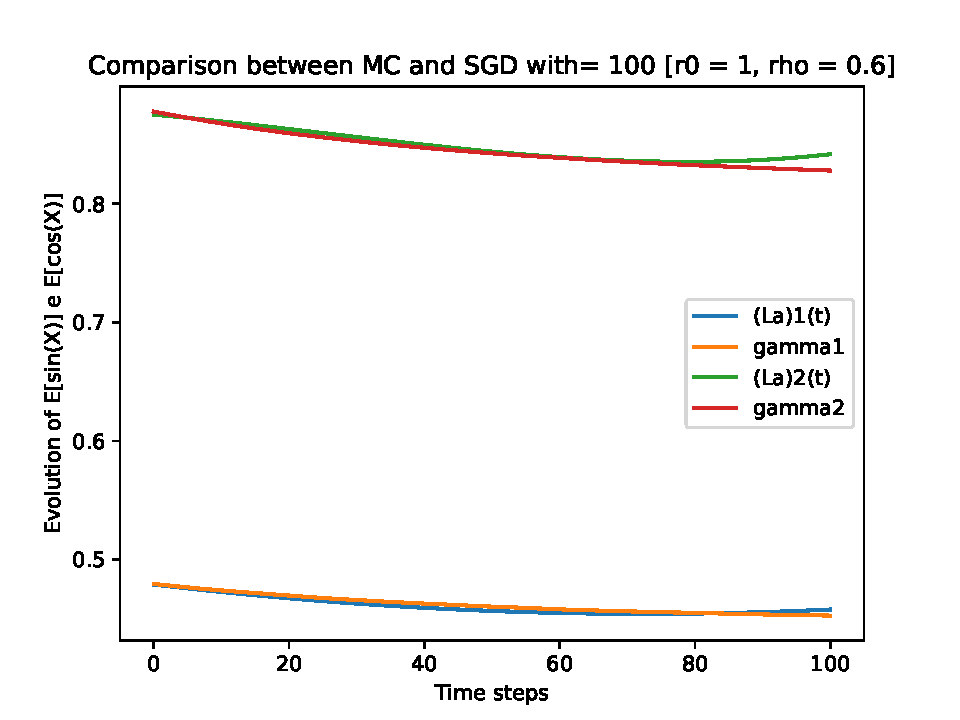
\includegraphics[width=0.9\textwidth]{images/graphics T = 1/n = 3, M = 100 sine and cosine.pdf}
\end{figure}
\begin{figure}[H]
\centering
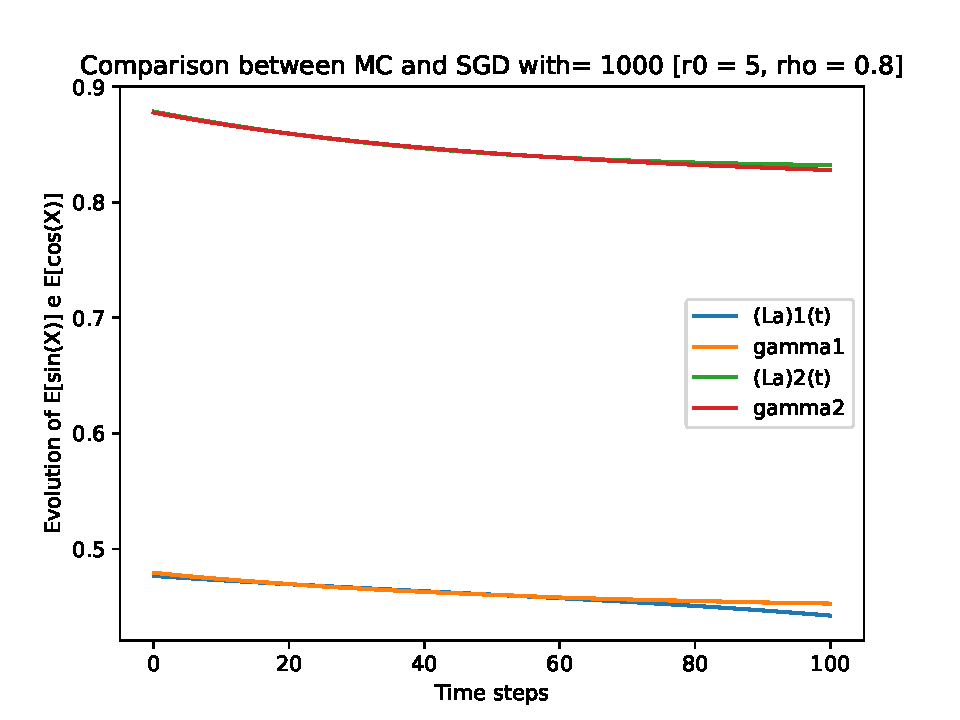
\includegraphics[width=0.9\textwidth]{images/graphics T = 1/n = 3, M = 1000 sine and cosine.pdf}
\end{figure}
\begin{figure}[H]
\centering
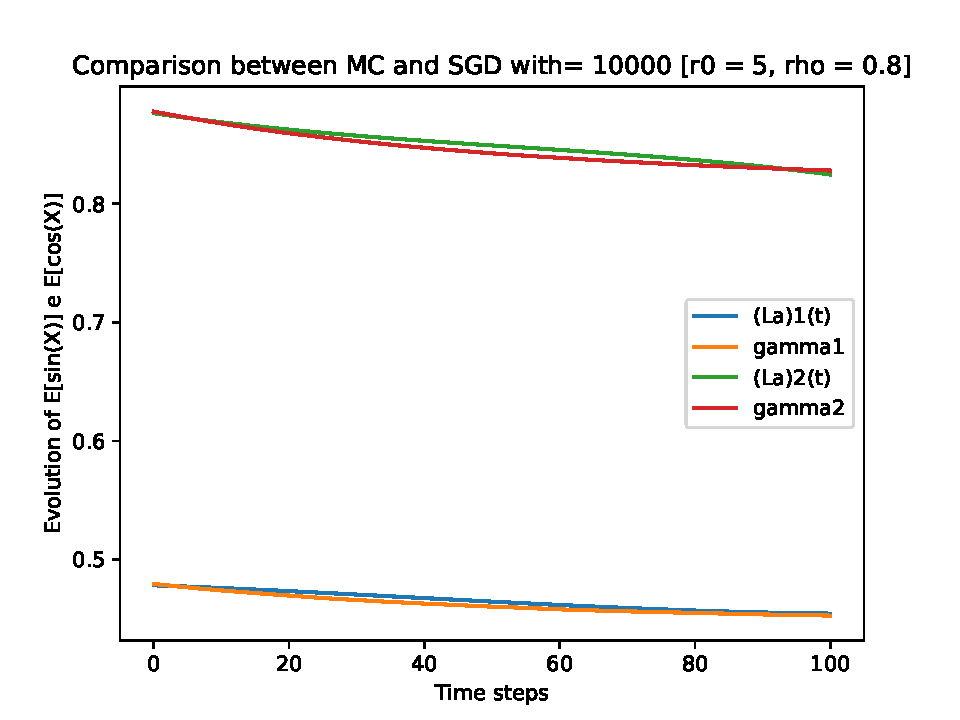
\includegraphics[width=0.9\textwidth]{images/graphics T = 1/n = 3, M = 10000 sine and cosine.pdf}
\end{figure}
\newpage
\section*{Caso n = 4} 
\begin{table}[H]
\centering
\addtolength{\leftskip}{-1.5cm}
\addtolength{\rightskip}{-1.5cm}
\begin{tabular}{|c|lll|}
\hline
$ $ & $r_0 = 1$ & $r_0 = 5$ & $r_0 = 10$ \\
\hline
$\rho = 0.6$ & 3.72 & 15.20 & 37.20 \\

$\rho = 0.7$ & 6.40 & 6.31 & 15.76 \\

$\rho = 0.8$ & 10.64 & 5.83 & 9.13 \\

$\rho = 0.9$ & 97.45 & 5.70 & 7.09 \\
\hline
\end{tabular}
\caption{Average execution
 times (in seconds $s$) with $M = 1$}
\end{table}
\begin{table}[H]
\centering
\addtolength{\leftskip}{-1.5cm}
\addtolength{\rightskip}{-1.5cm}
\begin{tabular}{|c|lllllllll|}
\hline
$ $ & $r_0 = 1$ & $r_0 = 1$ & $r_0 = 1$ & $r_0 = 5$ & $r_0 = 5$ & $r_0 = 5$ & $r_0 = 10$ & $r_0 = 10$ & $r_0 = 10$  \\
$ $ & min & max & average & min & max & average & min & max & average \\ 
\hline
$\rho = 0.6$ & 120 & 1280 & 517 & 1080 & 3820 & 2261 & 1830 & 8590 & 5523 \\

$\rho = 0.7$ & 290 & 3140 & 949 & 400 & 1500 & 942 & 540 & 4030 & 2334\\

$\rho = 0.8$ & 170 & 3520 & 1504 & 300 & 1270 & 869 & 440 & 2330 & 1346\\

$\rho = 0.9$ & 720 & 49999 & 14405.8 & 280 & 1960 & 848 & 380 & 1850 & 1047\\
\hline
\end{tabular}
\caption{Number of iterations $m$ to achieve convergence with $M = 1$}
\end{table}
\begin{table}[H]
\centering
\addtolength{\leftskip}{-1.5cm}
\addtolength{\rightskip}{-1.5cm}
\begin{tabular}{|c|lll|}
\hline
$ $ & $r_0 = 1$ & $r_0 = 5$ & $r_0 = 10$ \\
\hline
$\rho = 0.6$ & 0.92 & 2.69 & 6.23 \\

$\rho = 0.7$ & 0.96 & 1.72 & 7.68 \\

$\rho = 0.8$ & 2.55 & 1.45 & 5.01 \\

$\rho = 0.9$ & 17.99 & 1.39 & 3.59 \\
\hline
\end{tabular}
\caption{Average execution
 times (in seconds $s$) with $M = 10$}
\end{table}
\begin{table}[H]
\centering
\addtolength{\leftskip}{-1.5cm}
\addtolength{\rightskip}{-1.5cm}
\begin{tabular}{|c|lllllllll|}
\hline
$ $ & $r_0 = 1$ & $r_0 = 1$ & $r_0 = 1$ & $r_0 = 5$ & $r_0 = 5$ & $r_0 = 5$ & $r_0 = 10$ & $r_0 = 10$ & $r_0 = 10$  \\
$ $ & min & max & average & min & max & average & min & max & average \\ 
\hline
$\rho = 0.6$ & 50 & 180 & 117 & 110 & 590 & 340 & 260 & 890 & 548 \\

$\rho = 0.7$ & 10 & 300 & 123 & 100 & 660 & 219 & 190 & 530 & 369\\

$\rho = 0.8$ & 40 & 910 & 325 & 70 & 290 & 183 & 100 & 450 & 256\\

$\rho = 0.9$ & 40 & 11880 & 2280 & 20 & 520 & 177 & 60 & 310 & 180\\
\hline
\end{tabular}
\caption{Number of iterations $m$ to achieve convergence with $M = 10$}
\end{table}
\begin{table}[H]
\centering
\addtolength{\leftskip}{-1.5cm}
\addtolength{\rightskip}{-1.5cm}
\begin{tabular}{|c|lll|}
\hline
$ $ & $r_0 = 1$ & $r_0 = 5$ & $r_0 = 10$ \\
\hline
$\rho = 0.6$ & 1.36 & 2.10 & 3.85 \\

$\rho = 0.7$ & 1.81 & 1.36 & 2.15 \\

$\rho = 0.8$ & 1.61 & 1.74 & 1.55 \\

$\rho = 0.9$ & 1.33 & 1.11 & 1.45 \\
\hline
\end{tabular}
\caption{Average execution
 times (in seconds $s$) with $M = 100$}
\end{table}
\begin{table}[H]
\centering
\addtolength{\leftskip}{-1.5cm}
\addtolength{\rightskip}{-1.5cm}
\begin{tabular}{|c|lllllllll|}
\hline
$ $ & $r_0 = 1$ & $r_0 = 1$ & $r_0 = 1$ & $r_0 = 5$ & $r_0 = 5$ & $r_0 = 5$ & $r_0 = 10$ & $r_0 = 10$ & $r_0 = 10$  \\
$ $ & min & max & average & min & max & average & min & max & average \\ 
\hline
$\rho = 0.6$ & 10 & 130 & 40 & 20 & 150 & 62 & 60 & 140 & 106 \\

$\rho = 0.7$ & 20 & 260 & 55 & 10 & 100 & 39 & 20 & 150 & 61\\

$\rho = 0.8$ & 20 & 80 & 49 & 20 & 80 & 48 & 20 & 90 & 44\\

$\rho = 0.9$ & 10 & 120 & 41 & 10 & 60 & 31 & 20 & 60 & 41\\
\hline
\end{tabular}
\caption{Number of iterations $m$ to achieve convergence with $M = 100$}
\end{table}
\begin{table}[H]
\centering
\addtolength{\leftskip}{-1.5cm}
\addtolength{\rightskip}{-1.5cm}
\begin{tabular}{|c|lll|}
\hline
$ $ & $r_0 = 1$ & $r_0 = 5$ & $r_0 = 10$ \\
\hline
$\rho = 0.6$ & 2.17 & 1.38 & 3.64 \\

$\rho = 0.7$ & 2.24 & 1.33 & 2.73 \\

$\rho = 0.8$ & 3.97 & 1.31 & 2.31 \\

$\rho = 0.9$ & 5.90 & 1.08 & 1.85 \\
\hline
\end{tabular}
\caption{Average execution
 times (in seconds $s$) with $M = 1000$}
\end{table}
\begin{table}[H]
\centering
\addtolength{\leftskip}{-1.5cm}
\addtolength{\rightskip}{-1.5cm}
\begin{tabular}{|c|lllllllll|}
\hline
$ $ & $r_0 = 1$ & $r_0 = 1$ & $r_0 = 1$ & $r_0 = 5$ & $r_0 = 5$ & $r_0 = 5$ & $r_0 = 10$ & $r_0 = 10$ & $r_0 = 10$  \\
$ $ & min & max & average & min & max & average & min & max & average \\ 
\hline
$\rho = 0.6$ & 7 & 12 & 9.1 & 4 & 10 & 5.9 & 13 & 21 & 15.3 \\

$\rho = 0.7$ & 8 & 16 & 9.5 & 4 & 13 & 5.6 & 10 & 15 & 11.5 \\

$\rho = 0.8$ & 10 & 40 & 16.2 & 3 & 11 & 5.6 & 8 & 15 & 9.8 \\

$\rho = 0.9$ & 12 & 58 & 24.7 & 3 & 11 & 4.6 & 7 & 11 & 7.9\\
\hline
\end{tabular}
\caption{Number of iterations $m$ to achieve convergence with $M = 1000$}
\end{table}
\begin{table}[H]
\centering
\addtolength{\leftskip}{-1.5cm}
\addtolength{\rightskip}{-1.5cm}
\begin{tabular}{|c|lll|}
\hline
$ $ & $r_0 = 1$ & $r_0 = 5$ & $r_0 = 10$ \\
\hline
$\rho = 0.6$ & 17.09 & 10.90 & 33.12 \\

$\rho = 0.7$ & 20.29 & 9.95 & 24.45 \\

$\rho = 0.8$ & 25.10 & 9.10 & 16.95 \\

$\rho = 0.9$ & 32.85 & 8.00 & 7.84 \\
\hline
\end{tabular}
\caption{Average execution
 times (in seconds $s$) with $M = 10000$}
\end{table}
\begin{table}[H]
\centering
\addtolength{\leftskip}{-1.5cm}
\addtolength{\rightskip}{-1.5cm}
\begin{tabular}{|c|lllllllll|}
\hline
$ $ & $r_0 = 1$ & $r_0 = 1$ & $r_0 = 1$ & $r_0 = 5$ & $r_0 = 5$ & $r_0 = 5$ & $r_0 = 10$ & $r_0 = 10$ & $r_0 = 10$  \\
$ $ & min & max & average & min & max & average & min & max & average \\ 
\hline
$\rho = 0.6$ & 7 & 7 & 7 & 4 & 5 & 4.4 & 13 & 14 & 13.3 \\

$\rho = 0.7$ & 7 & 9 & 8.3 & 4 & 4 & 4 & 10 & 10 & 10\\

$\rho = 0.8$ & 9 & 13 & 10.2 & 3 & 4 & 3.7 & 8 & 8 & 8\\

$\rho = 0.9$ & 12 & 15 & 13.3 & 3 & 3 & 3 & 7 & 7 & 7\\
\hline
\end{tabular}
\caption{Number of iterations $m$ to achieve convergence with $M = 10000$}
\end{table}
\begin{figure}[H]
\centering
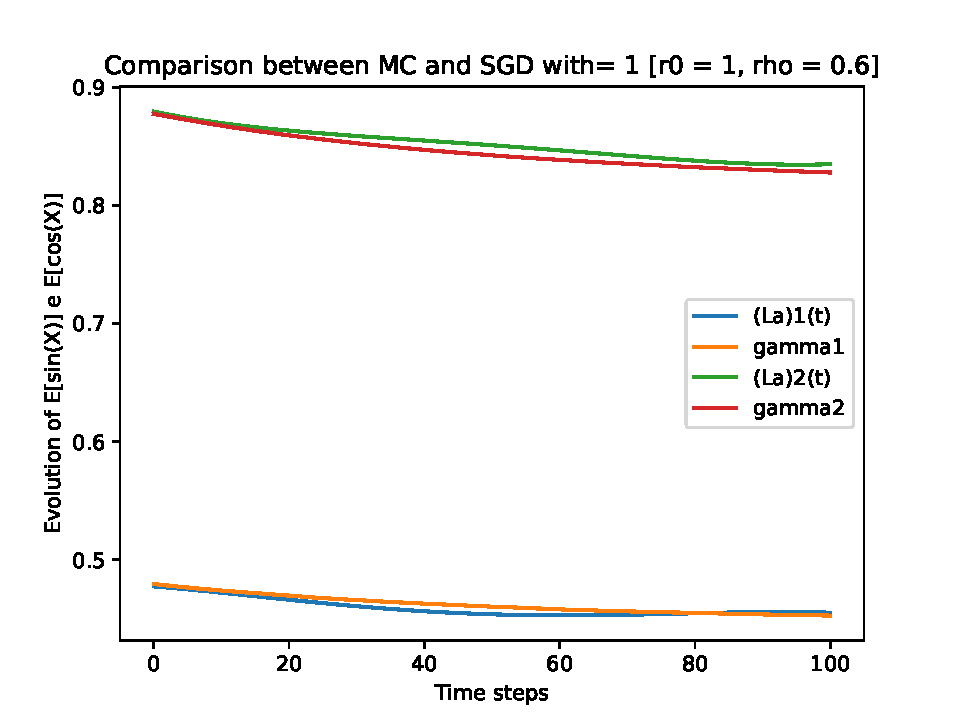
\includegraphics[width=0.9\textwidth]{images/graphics T = 1/n = 4, M = 1 sine and cosine.pdf}
\end{figure}
\begin{figure}[H]
\centering
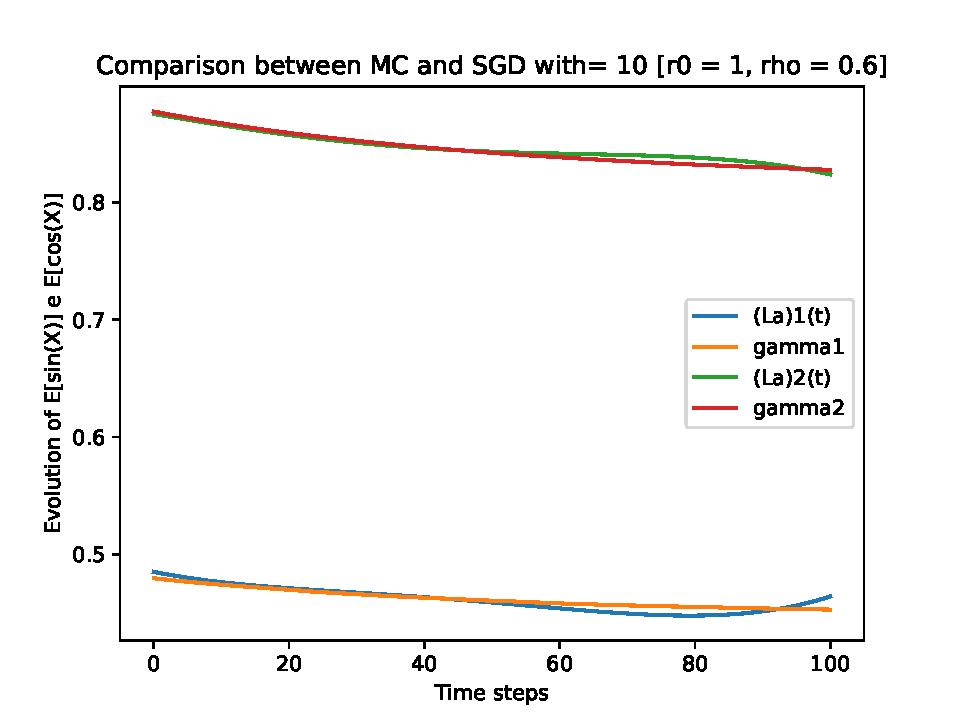
\includegraphics[width=0.9\textwidth]{images/graphics T = 1/n = 4, M = 10 sine and cosine.pdf}
\end{figure}
\begin{figure}[H]
\centering
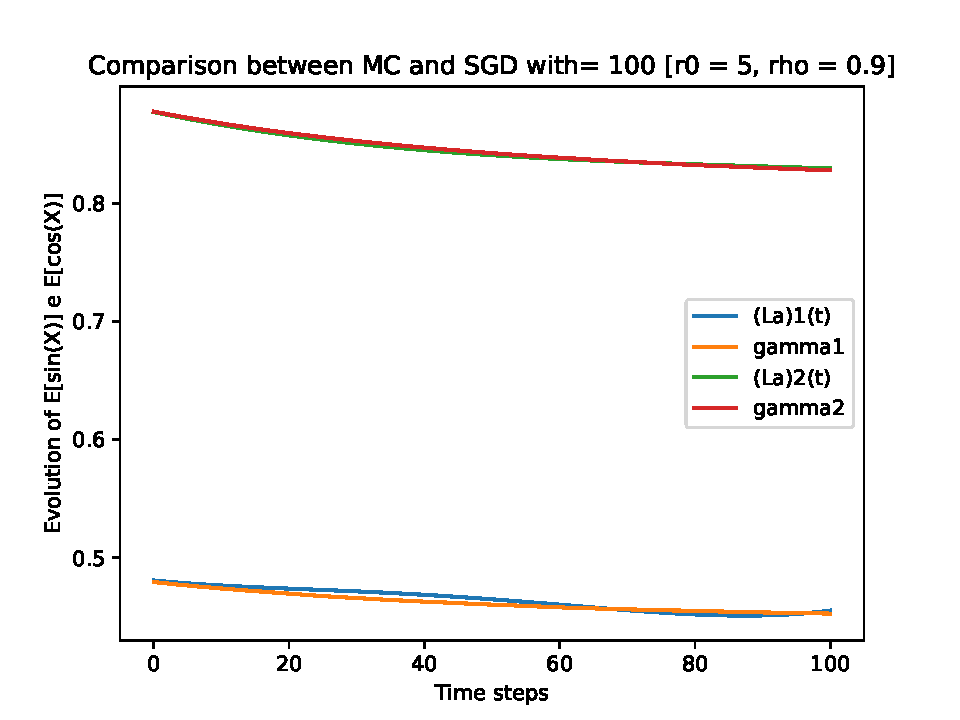
\includegraphics[width=0.9\textwidth]{images/graphics T = 1/n = 4, M = 100 sine and cosine.pdf}
\end{figure}
\begin{figure}[H]
\centering
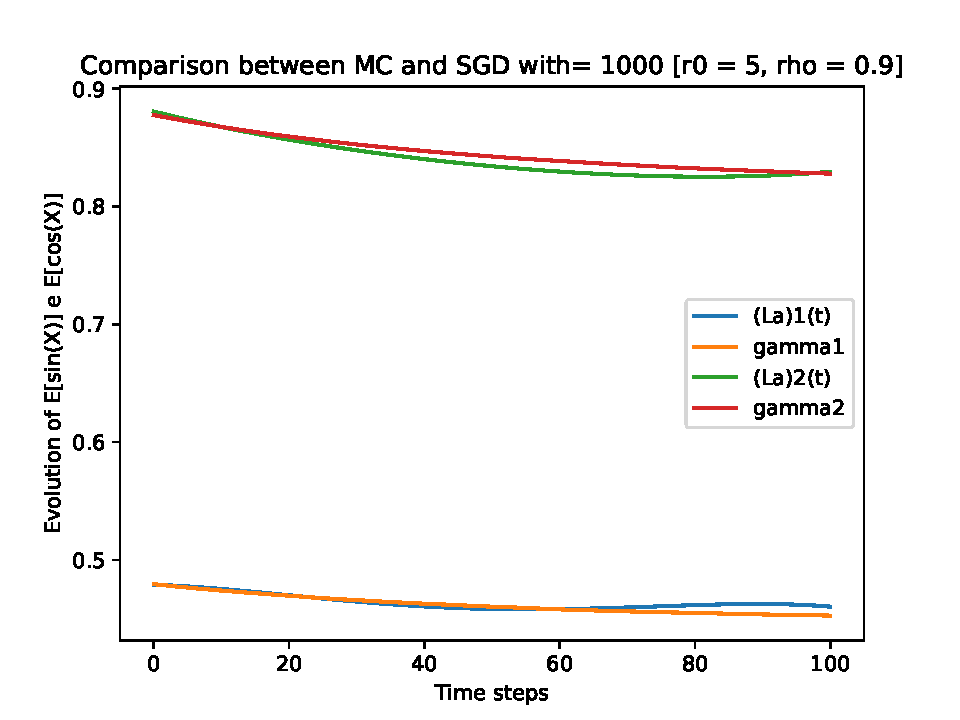
\includegraphics[width=0.9\textwidth]{images/graphics T = 1/n = 4, M = 1000 sine and cosine.pdf}
\end{figure}
\begin{figure}[H]
\centering
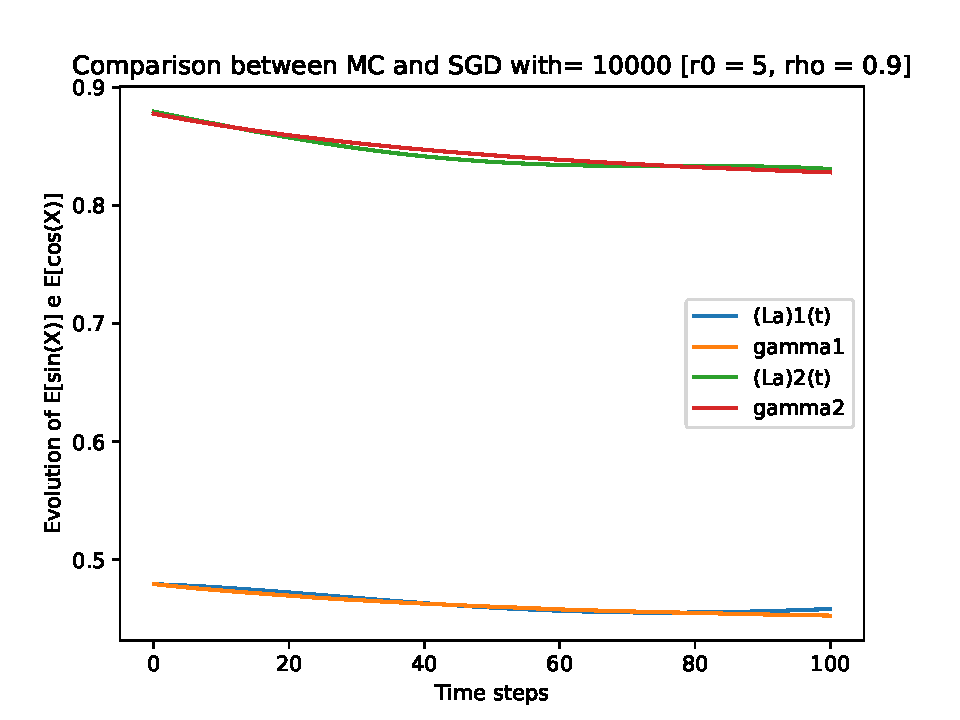
\includegraphics[width=0.9\textwidth]{images/graphics T = 1/n = 4, M = 10000 sine and cosine.pdf}
\end{figure}
\newpage
\section*{Caso n = 5} 
\begin{table}[H]
\centering
\addtolength{\leftskip}{-1.5cm}
\addtolength{\rightskip}{-1.5cm}
\begin{tabular}{|c|lll|}
\hline
$ $ & $r_0 = 1$ & $r_0 = 5$ & $r_0 = 10$ \\
\hline
$\rho = 0.6$ & 4.81 & 14.76 & 31.03 \\

$\rho = 0.7$ & 9.11 & 7.29 & 17.28 \\

$\rho = 0.8$ & 31.30 & 5.37 & 10.54 \\

$\rho = 0.9$ & 90.16 & 6.65 & 5.83 \\
\hline
\end{tabular}
\caption{Average execution
 times (in seconds $s$) with $M = 1$}
\end{table}
\begin{table}[H]
\centering
\addtolength{\leftskip}{-1.5cm}
\addtolength{\rightskip}{-1.5cm}
\begin{tabular}{|c|lllllllll|}
\hline
$ $ & $r_0 = 1$ & $r_0 = 1$ & $r_0 = 1$ & $r_0 = 5$ & $r_0 = 5$ & $r_0 = 5$ & $r_0 = 10$ & $r_0 = 10$ & $r_0 = 10$  \\
$ $ & min & max & average & min & max & average & min & max & average \\ 
\hline
$\rho = 0.6$ & 340 & 1340 & 709 & 1670 & 3170 & 2166 & 1690 & 8820 & 4546 \\

$\rho = 0.7$ & 410 & 2260 & 1323 & 160 & 2300 & 1071 & 770 & 4350 & 2533\\

$\rho = 0.8$ & 240 & 24910 & 4579 & 90 & 1650 & 789 & 820 & 2910 & 1543\\

$\rho = 0.9$ & 570 & 49999 & 13249.9 & 470 & 1860 & 978 & 380 & 1350 & 857\\
\hline
\end{tabular}
\caption{Number of iterations $m$ to achieve convergence with $M = 1$}
\end{table}
\begin{table}[H]
\centering
\addtolength{\leftskip}{-1.5cm}
\addtolength{\rightskip}{-1.5cm}
\begin{tabular}{|c|lll|}
\hline
$ $ & $r_0 = 1$ & $r_0 = 5$ & $r_0 = 10$ \\
\hline
$\rho = 0.6$ & 1.42 & 1.65 & 4.35 \\

$\rho = 0.7$ & 1.71 & 1.87 &  2.07 \\

$\rho = 0.8$ & 3.27 & 1.42 & 1.88 \\

$\rho = 0.9$ & 1.47 & 1.26 & 1.81 \\
\hline
\end{tabular}
\caption{Average execution
 times (in seconds $s$) with $M = 10$}
\end{table}
\begin{table}[H]
\centering
\addtolength{\leftskip}{-1.5cm}
\addtolength{\rightskip}{-1.5cm}
\begin{tabular}{|c|lllllllll|}
\hline
$ $ & $r_0 = 1$ & $r_0 = 1$ & $r_0 = 1$ & $r_0 = 5$ & $r_0 = 5$ & $r_0 = 5$ & $r_0 = 10$ & $r_0 = 10$ & $r_0 = 10$  \\
$ $ & min & max & average & min & max & average & min & max & average \\ 
\hline
$\rho = 0.6$ & 50 & 580 & 179 & 80 & 420 & 206 & 120 & 870 & 540 \\

$\rho = 0.7$ & 60 & 1180 & 216 & 80 & 430 & 235 & 120 & 570 & 257\\

$\rho = 0.8$ & 50 & 1460 & 411 & 140 & 330 & 178 & 70 & 390 & 235\\

$\rho = 0.9$ & 40 & 750 & 185 & 50 & 370 & 157 & 90 & 490 & 228\\
\hline
\end{tabular}
\caption{Number of iterations $m$ to achieve convergence with $M = 10$}
\end{table}
\begin{table}[H]
\centering
\addtolength{\leftskip}{-1.5cm}
\addtolength{\rightskip}{-1.5cm}
\begin{tabular}{|c|lll|}
\hline
$ $ & $r_0 = 1$ & $r_0 = 5$ & $r_0 = 10$ \\
\hline
$\rho = 0.6$ & 0.66 & 0.47 & 1.23 \\

$\rho = 0.7$ & 0.63 & 0.69 & 0.87 \\

$\rho = 0.8$ & 0.73 & 0.39 & 0.95 \\

$\rho = 0.9$ & 1.93 & 0.49 & 0.43 \\
\hline
\end{tabular}
\caption{Average execution
 times (in seconds $s$) with $M = 100$}
\end{table}
\begin{table}[H]
\centering
\addtolength{\leftskip}{-1.5cm}
\addtolength{\rightskip}{-1.5cm}
\begin{tabular}{|c|lllllllll|}
\hline
$ $ & $r_0 = 1$ & $r_0 = 1$ & $r_0 = 1$ & $r_0 = 5$ & $r_0 = 5$ & $r_0 = 5$ & $r_0 = 10$ & $r_0 = 10$ & $r_0 = 10$  \\
$ $ & min & max & average & min & max & average & min & max & average \\ 
\hline
$\rho = 0.6$ & 20 & 100 & 46 & 10 & 60 & 33 & 30 & 150 & 86 \\

$\rho = 0.7$ & 20 & 150 & 44 & 10 & 130 & 48 & 20 & 90 & 61\\

$\rho = 0.8$ & 20 & 180 & 51 & 10 & 40 & 27 & 30 & 110 & 66\\

$\rho = 0.9$ & 40 & 370 & 135 & 10 & 90 & 34 & 10 & 60 & 30\\
\hline
\end{tabular}
\caption{Number of iterations $m$ to achieve convergence with $M = 100$}
\end{table}
\begin{table}[H]
\centering
\addtolength{\leftskip}{-1.5cm}
\addtolength{\rightskip}{-1.5cm}
\begin{tabular}{|c|lll|}
\hline
$ $ & $r_0 = 1$ & $r_0 = 5$ & $r_0 = 10$ \\
\hline
$\rho = 0.6$ & 1.35 & 0.67 & 1.37 \\

$\rho = 0.7$ & 1.48 & 0.52 & 0.92 \\

$\rho = 0.8$ & 2.33 & 0.37 & 0.87 \\

$\rho = 0.9$ & 3.61 & 0.53 & 0.74 \\
\hline
\end{tabular}
\caption{Average execution
 times (in seconds $s$) with $M = 1000$}
\end{table}
\begin{table}[H]
\centering
\addtolength{\leftskip}{-1.5cm}
\addtolength{\rightskip}{-1.5cm}
\begin{tabular}{|c|lllllllll|}
\hline
$ $ & $r_0 = 1$ & $r_0 = 1$ & $r_0 = 1$ & $r_0 = 5$ & $r_0 = 5$ & $r_0 = 5$ & $r_0 = 10$ & $r_0 = 10$ & $r_0 = 10$  \\
$ $ & min & max & average & min & max & average & min & max & average \\ 
\hline
$\rho = 0.6$ & 10 & 18 & 12.3 & 3 & 14 & 6.1 & 10 & 15 & 12.5 \\

$\rho = 0.7$ & 11 & 16 & 13.4 & 3 & 8 & 4.7 & 8 & 10 & 8.4 \\

$\rho = 0.8$ & 17 & 27 & 21.1 & 3 & 4 & 3.3 & 6 & 12 & 7.9 \\

$\rho = 0.9$ & 23 & 66 & 32.9 & 3 & 11 & 4.8 & 6 & 8 & 6.7\\
\hline
\end{tabular}
\caption{Number of iterations $m$ to achieve convergence with $M = 1000$}
\end{table}
\begin{table}[H]
\centering
\addtolength{\leftskip}{-1.5cm}
\addtolength{\rightskip}{-1.5cm}
\begin{tabular}{|c|lll|}
\hline
$ $ & $r_0 = 1$ & $r_0 = 5$ & $r_0 = 10$ \\
\hline
$\rho = 0.6$ & 13.12 & 4.45 & 13.18 \\

$\rho = 0.7$ & 15.57 & 3.89 & 10.47 \\

$\rho = 0.8$ & 20.77 & 3.93 & 8.27 \\

$\rho = 0.9$ & 31.73 & 3.90 & 7.20 \\
\hline
\end{tabular}
\caption{Average execution
 times (in seconds $s$) with $M = 10000$}
\end{table}
\begin{table}[H]
\centering
\addtolength{\leftskip}{-1.5cm}
\addtolength{\rightskip}{-1.5cm}
\begin{tabular}{|c|lllllllll|}
\hline
$ $ & $r_0 = 1$ & $r_0 = 1$ & $r_0 = 1$ & $r_0 = 5$ & $r_0 = 5$ & $r_0 = 5$ & $r_0 = 10$ & $r_0 = 10$ & $r_0 = 10$  \\
$ $ & min & max & average & min & max & average & min & max & average \\ 
\hline
$\rho = 0.6$ & 9 & 11 & 10 & 3 & 4 & 3.4 & 10 & 11 & 10.1 \\

$\rho = 0.7$ & 11 & 13 & 11.9 & 3 & 3 & 3 & 8 & 8 & 8\\

$\rho = 0.8$ & 15 & 16 & 15.9 & 3 & 3 & 3 & 6 & 7 & 6.3\\

$\rho = 0.9$ & 22 & 31 & 24.3 & 3 & 3 & 3 & 5 & 6 & 5.5\\
\hline
\end{tabular}
\caption{Number of iterations $m$ to achieve convergence with $M = 10000$}
\end{table}
\begin{figure}[H]
\centering
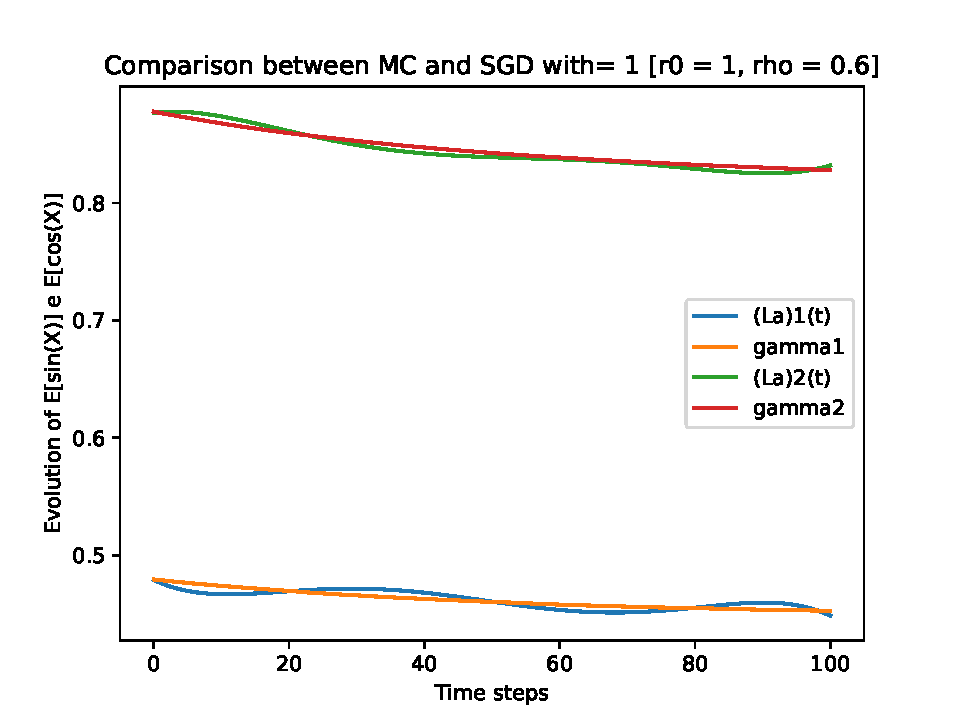
\includegraphics[width=0.9\textwidth]{images/graphics T = 1/n = 5, M = 1 sine and cosine.pdf}
\end{figure}
\begin{figure}[H]
\centering
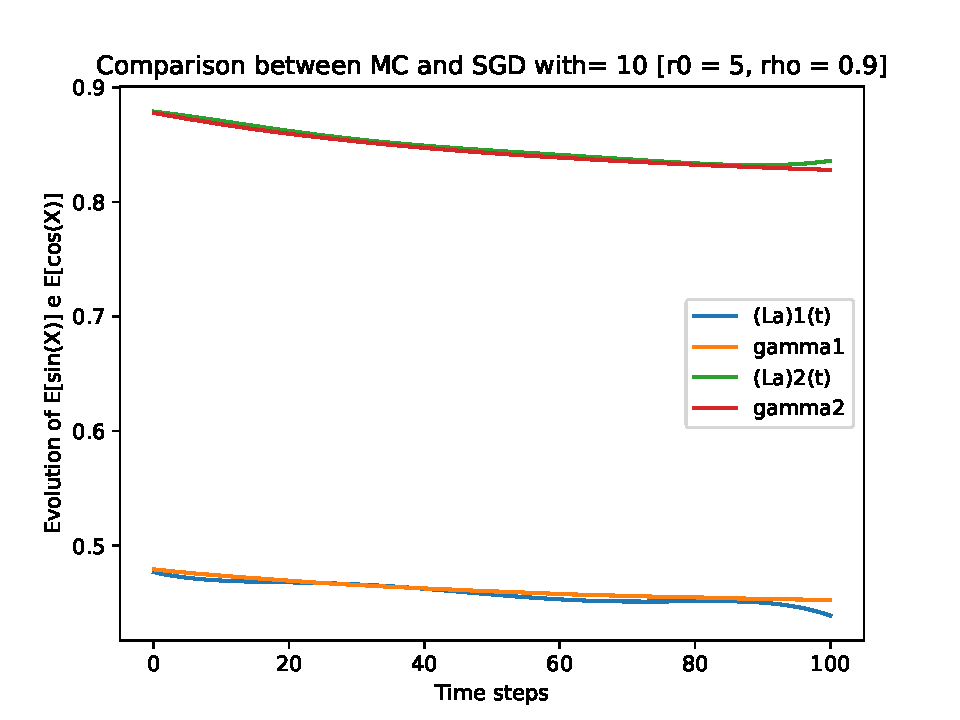
\includegraphics[width=0.9\textwidth]{images/graphics T = 1/n = 5, M = 10 sine and cosine.pdf}
\end{figure}
\begin{figure}[H]
\centering
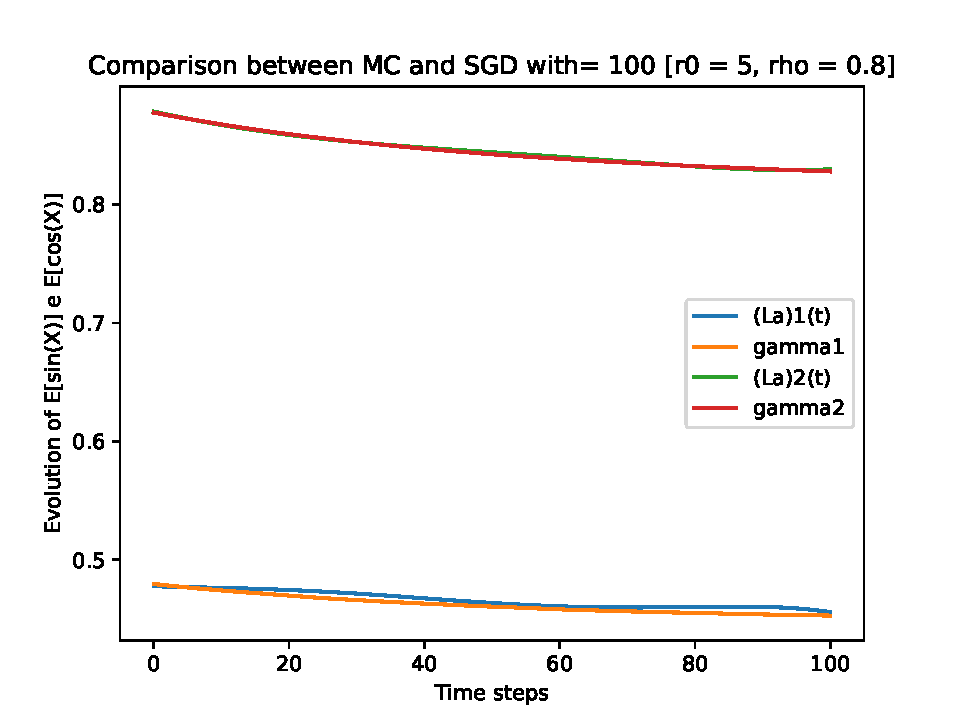
\includegraphics[width=0.9\textwidth]{images/graphics T = 1/n = 5, M = 100 sine and cosine.pdf}
\end{figure}
\begin{figure}[H]
\centering
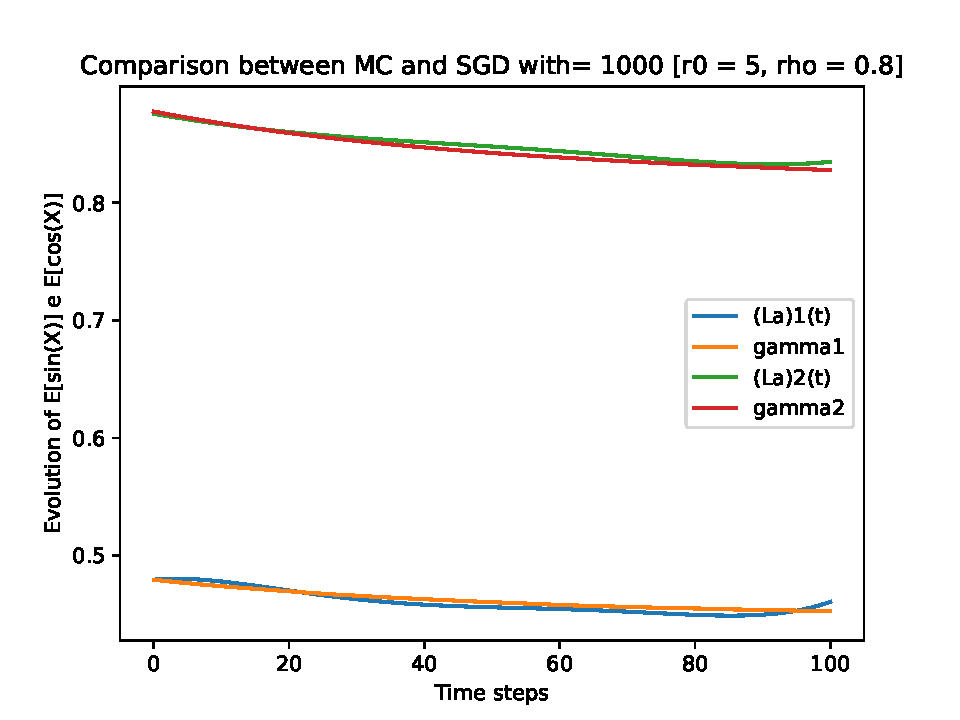
\includegraphics[width=0.9\textwidth]{images/graphics T = 1/n = 5, M = 1000 sine and cosine.pdf}
\end{figure}
\begin{figure}[H]
\centering
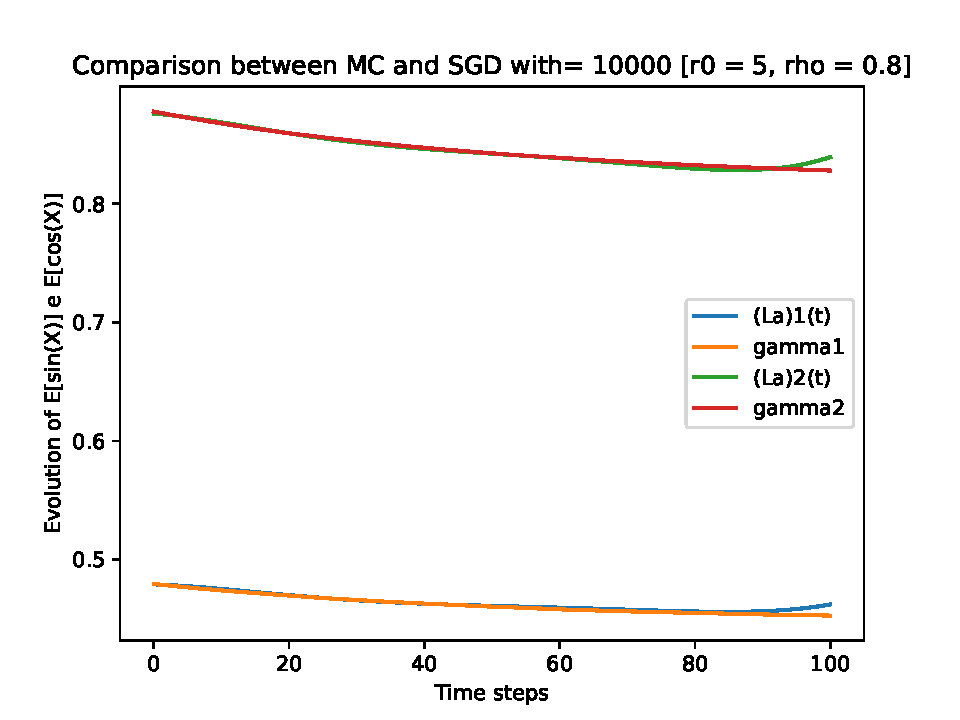
\includegraphics[width=0.9\textwidth]{images/graphics T = 1/n = 5, M = 10000 sine and cosine.pdf}
\end{figure}
\newpage
\section*{Caso n = 6} 
\begin{table}[H]
\centering
\addtolength{\leftskip}{-1.5cm}
\addtolength{\rightskip}{-1.5cm}
\begin{tabular}{|c|lll|}
\hline
$ $ & $r_0 = 1$ & $r_0 = 5$ & $r_0 = 10$ \\
\hline
$\rho = 0.6$ & 7.97 & 13.95 & 35.22 \\

$\rho = 0.7$ & 11.89 & 9.05 & 18.96 \\

$\rho = 0.8$ & 17.13 & 10.48 & 9.50 \\

$\rho = 0.9$ & 157.41 & 10.32 & 6.82 \\
\hline
\end{tabular}
\caption{Average execution
 times (in seconds $s$) with $M = 1$}
\end{table}
\begin{table}[H]
\centering
\addtolength{\leftskip}{-1.5cm}
\addtolength{\rightskip}{-1.5cm}
\begin{tabular}{|c|lllllllll|}
\hline
$ $ & $r_0 = 1$ & $r_0 = 1$ & $r_0 = 1$ & $r_0 = 5$ & $r_0 = 5$ & $r_0 = 5$ & $r_0 = 10$ & $r_0 = 10$ & $r_0 = 10$  \\
$ $ & min & max & average & min & max & average & min & max & average \\ 
\hline
$\rho = 0.6$ & 170 & 1920 & 1142 & 610 & 3310 & 1991 & 2510 & 9890 & 5037 \\

$\rho = 0.7$ & 320 & 6730 & 1702 & 210 & 2550 & 1292 & 770 & 3790 & 2713\\

$\rho = 0.8$ & 390 & 10610 & 2453 & 500 & 3180 & 1501 & 540 & 2200 & 1359\\

$\rho = 0.9$ & 590 & 49999 & 22514.8 & 430 & 5640 & 1475 & 380 & 2510 & 976\\
\hline
\end{tabular}
\caption{Number of iterations $m$ to achieve convergence with $M = 1$}
\end{table}
\begin{table}[H]
\centering
\addtolength{\leftskip}{-1.5cm}
\addtolength{\rightskip}{-1.5cm}
\begin{tabular}{|c|lll|}
\hline
$ $ & $r_0 = 1$ & $r_0 = 5$ & $r_0 = 10$ \\
\hline
$\rho = 0.6$ & 1.13 & 2.55 & 6.69 \\

$\rho = 0.7$ & 2.00 & 2.10 & 4.14 \\

$\rho = 0.8$ & 5.07 & 2.23 & 2.89 \\

$\rho = 0.9$ & 19.58 & 1.94 & 2.00 \\
\hline
\end{tabular}
\caption{Average execution
 times (in seconds $s$) with $M = 10$}
\end{table}
\begin{table}[H]
\centering
\addtolength{\leftskip}{-1.5cm}
\addtolength{\rightskip}{-1.5cm}
\begin{tabular}{|c|lllllllll|}
\hline
$ $ & $r_0 = 1$ & $r_0 = 1$ & $r_0 = 1$ & $r_0 = 5$ & $r_0 = 5$ & $r_0 = 5$ & $r_0 = 10$ & $r_0 = 10$ & $r_0 = 10$  \\
$ $ & min & max & average & min & max & average & min & max & average \\ 
\hline
$\rho = 0.6$ & 40 & 220 & 96 & 100 & 420 & 216 & 230 & 880 & 565 \\

$\rho = 0.7$ & 30 & 430 & 171 & 70 & 330 & 178 & 130 & 580 & 351\\

$\rho = 0.8$ & 40 & 1560 & 431 & 70 & 550 & 187 & 70 & 360 & 246\\

$\rho = 0.9$ & 100 & 6200 & 1661 & 60 & 270 & 164 & 70 & 330 & 170\\
\hline
\end{tabular}
\caption{Number of iterations $m$ to achieve convergence with $M = 10$}
\end{table}
\begin{table}[H]
\centering
\addtolength{\leftskip}{-1.5cm}
\addtolength{\rightskip}{-1.5cm}
\begin{tabular}{|c|lll|}
\hline
$ $ & $r_0 = 1$ & $r_0 = 5$ & $r_0 = 10$ \\
\hline
$\rho = 0.6$ & 0.62 & 0.72 & 1.11 \\

$\rho = 0.7$ & 0.86 & 0.52 & 0.85 \\

$\rho = 0.8$ & 1.57 & 0.34 & 0.73 \\

$\rho = 0.9$ & 1.55 & 0.54 & 0.46 \\
\hline
\end{tabular}
\caption{Average execution
 times (in seconds $s$) with $M = 100$}
\end{table}
\begin{table}[H]
\centering
\addtolength{\leftskip}{-1.5cm}
\addtolength{\rightskip}{-1.5cm}
\begin{tabular}{|c|lllllllll|}
\hline
$ $ & $r_0 = 1$ & $r_0 = 1$ & $r_0 = 1$ & $r_0 = 5$ & $r_0 = 5$ & $r_0 = 5$ & $r_0 = 10$ & $r_0 = 10$ & $r_0 = 10$  \\
$ $ & min & max & average & min & max & average & min & max & average \\ 
\hline
$\rho = 0.6$ & 20 & 110 & 40 & 10 & 110 & 47 & 40 & 110 & 72\\

$\rho = 0.7$ & 30 & 140 & 56 & 20 & 60 & 34 & 30 & 70 & 55\\

$\rho = 0.8$ & 40 & 300 & 102 & 10 & 40 & 22 & 10 & 70 & 47\\

$\rho = 0.9$ & 40 & 320 & 100 & 10 & 100 & 35 & 10 & 60 & 30\\
\hline
\end{tabular}
\caption{Number of iterations $m$ to achieve convergence with $M = 100$}
\end{table}
\begin{table}[H]
\centering
\addtolength{\leftskip}{-1.5cm}
\addtolength{\rightskip}{-1.5cm}
\begin{tabular}{|c|lll|}
\hline
$ $ & $r_0 = 1$ & $r_0 = 5$ & $r_0 = 10$ \\
\hline
$\rho = 0.6$ & 2.18 & 0.55 & 1.05 \\

$\rho = 0.7$ & 2.51 & 0.53 & 0.89 \\

$\rho = 0.8$ & 3.59 & 0.52 & 1.00 \\

$\rho = 0.9$ & 6.78 & 0.48 & 0.73 \\
\hline
\end{tabular}
\caption{Average execution
 times (in seconds $s$) with $M = 1000$}
\end{table}
\begin{table}[H]
\centering
\addtolength{\leftskip}{-1.5cm}
\addtolength{\rightskip}{-1.5cm}
\begin{tabular}{|c|lllllllll|}
\hline
$ $ & $r_0 = 1$ & $r_0 = 1$ & $r_0 = 1$ & $r_0 = 5$ & $r_0 = 5$ & $r_0 = 5$ & $r_0 = 10$ & $r_0 = 10$ & $r_0 = 10$  \\
$ $ & min & max & average & min & max & average & min & max & average \\ 
\hline
$\rho = 0.6$ & 14 & 23 & 17.7 & 3 & 7 & 4.5 & 8 & 11 & 8.6 \\

$\rho = 0.7$ & 16 & 26 & 20.4 & 3 & 8 & 4.2 & 6 & 9 & 7.2 \\

$\rho = 0.8$ & 24 & 45 & 29.2 & 2 & 8 & 4.2 & 5 & 17 & 7.9 \\

$\rho = 0.9$ & 38 & 111 & 54.9 & 3 & 6 & 3.9 & 5 & 7 & 5.9\\
\hline
\end{tabular}
\caption{Number of iterations $m$ to achieve convergence with $M = 1000$}
\end{table}
\begin{table}[H]
\centering
\addtolength{\leftskip}{-1.5cm}
\addtolength{\rightskip}{-1.5cm}
\begin{tabular}{|c|lll|}
\hline
$ $ & $r_0 = 1$ & $r_0 = 5$ & $r_0 = 10$ \\
\hline
$\rho = 0.6$ & 20.21 & 4.72 & 12.51 \\

$\rho = 0.7$ & 27.02 & 4.22 & 9.48 \\

$\rho = 0.8$ & 39.52 & 3.61 & 7.80 \\

$\rho = 0.9$ & 66.18 & 3.11 & 7.78 \\
\hline
\end{tabular}
\caption{Average execution
 times (in seconds $s$) with $M = 10000$}
\end{table}
\begin{table}[H]
\centering
\addtolength{\leftskip}{-1.5cm}
\addtolength{\rightskip}{-1.5cm}
\begin{tabular}{|c|lllllllll|}
\hline
$ $ & $r_0 = 1$ & $r_0 = 1$ & $r_0 = 1$ & $r_0 = 5$ & $r_0 = 5$ & $r_0 = 5$ & $r_0 = 10$ & $r_0 = 10$ & $r_0 = 10$  \\
$ $ & min & max & average & min & max & average & min & max & average \\ 
\hline
$\rho = 0.6$ & 12 & 14 & 12.9 & 3 & 3 & 3 & 8 & 8 & 8 \\

$\rho = 0.7$ & 16 & 19 & 17.2 & 2 & 3 & 2.7 & 6 & 7 & 6.1\\

$\rho = 0.8$ & 23 & 28 & 25.3 & 2 & 3 & 2.3 & 5 & 5 & 5\\

$\rho = 0.9$ & 41 & 45 & 42.3 & 2 & 2 & 2 & 5 & 5 & 5\\
\hline
\end{tabular}
\caption{Number of iterations $m$ to achieve convergence with $M = 10000$}
\end{table}
\begin{figure}[H]
\centering
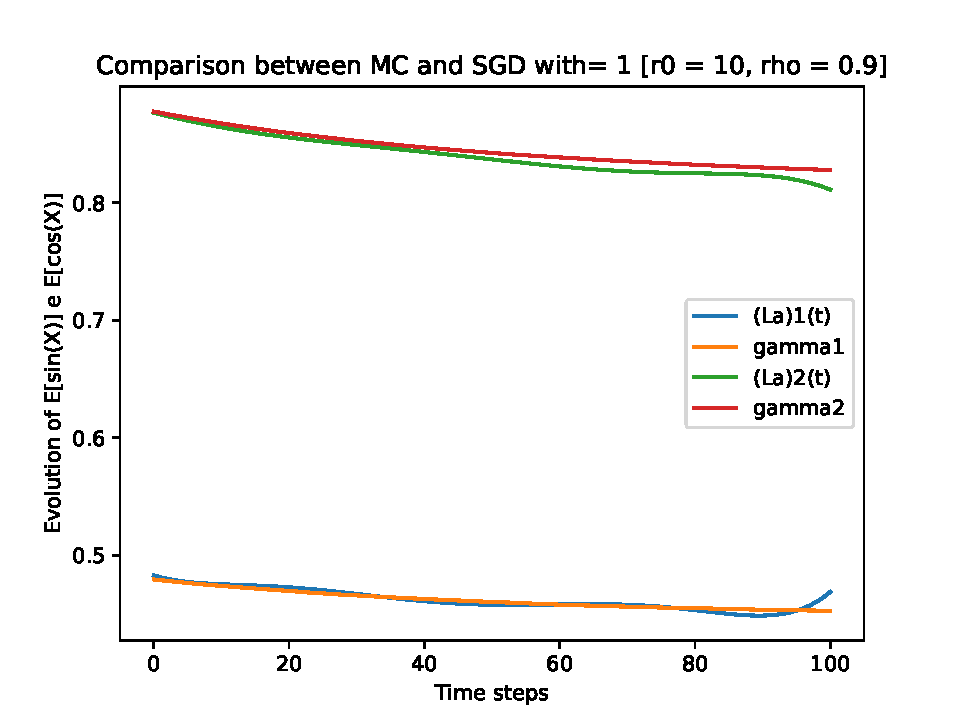
\includegraphics[width=0.9\textwidth]{images/graphics T = 1/n = 6, M = 1 sine and cosine.pdf}
\end{figure}
\begin{figure}[H]
\centering
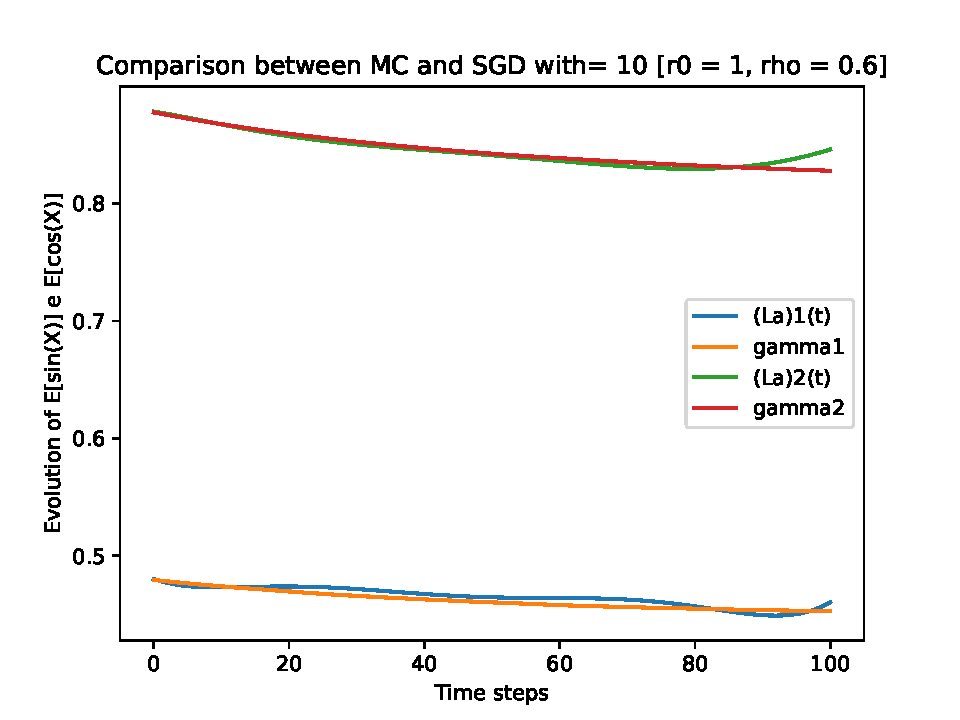
\includegraphics[width=0.9\textwidth]{images/graphics T = 1/n = 6, M = 10 sine and cosine.pdf}
\end{figure}
\begin{figure}[H]
\centering
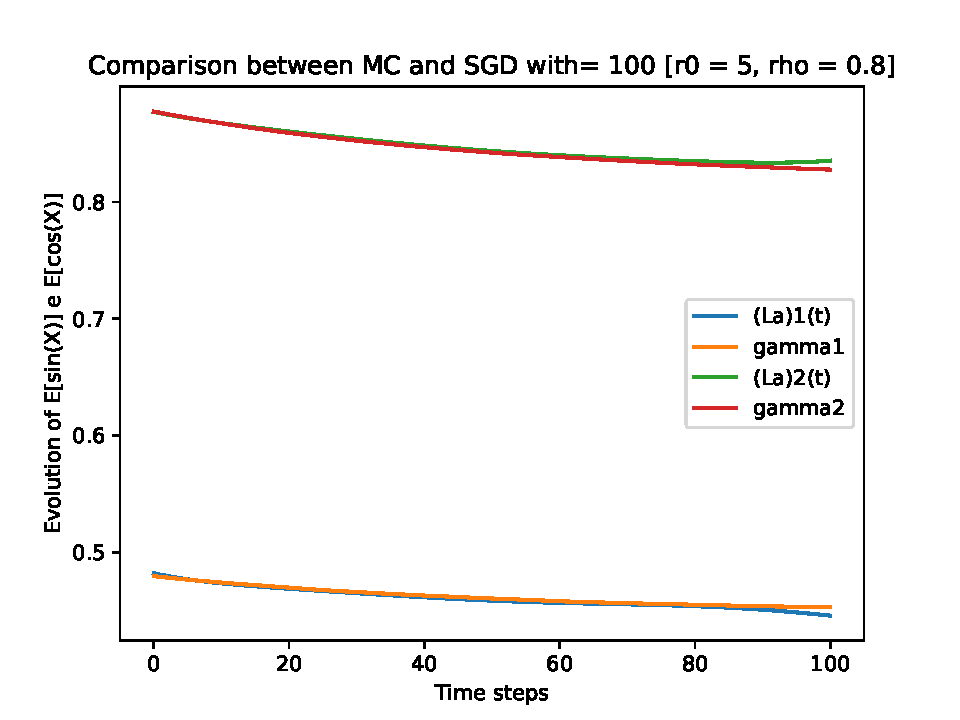
\includegraphics[width=0.9\textwidth]{images/graphics T = 1/n = 6, M = 100 sine and cosine.pdf}
\end{figure}
\begin{figure}[H]
\centering
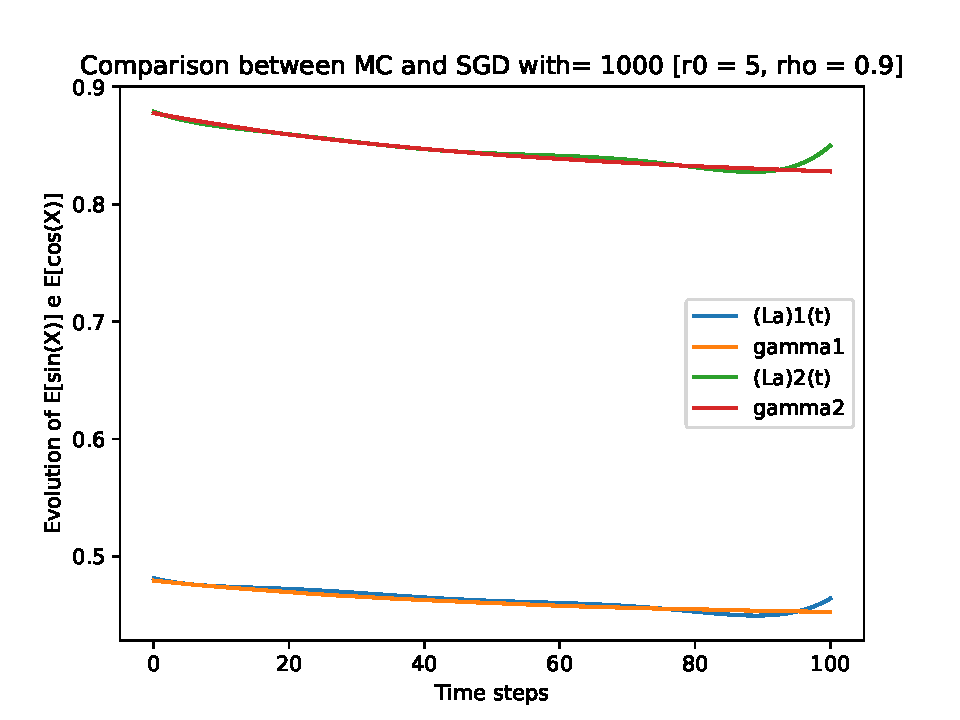
\includegraphics[width=0.9\textwidth]{images/graphics T = 1/n = 6, M = 1000 sine and cosine.pdf}
\end{figure}
\begin{figure}[H]
\centering
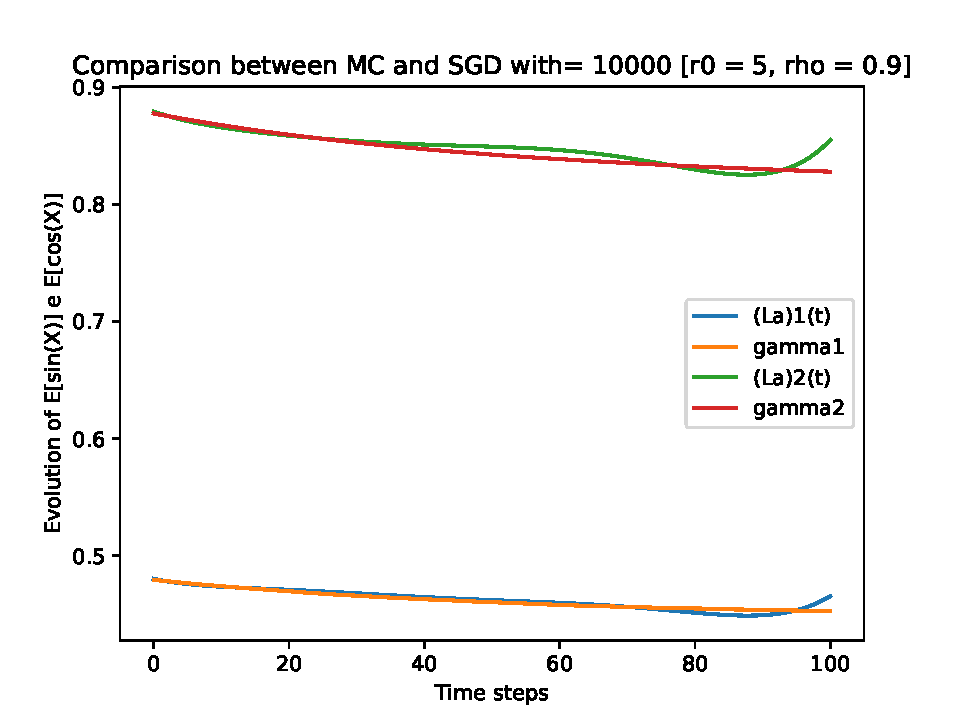
\includegraphics[width=0.9\textwidth]{images/graphics T = 1/n = 6, M = 10000 sine and cosine.pdf}
\end{figure}
\newpage
\section{T = 2}
\section*{Caso n = 3} 
\begin{table}[H]
\centering
\addtolength{\leftskip}{-1.5cm}
\addtolength{\rightskip}{-1.5cm}
\begin{tabular}{|c|ll|}
\hline
$ $ & $r_0 = 1$ & $r_0 = 5$ \\
\hline
$\rho = 0.6$ & 22.35 & 80.57 \\

$\rho = 0.7$ & 12.28 & 42.48 \\

$\rho = 0.8$ & 34.07 & 19.80 \\

$\rho = 0.9$ & 94.34 & 23.10 \\
\hline
\end{tabular}
\caption{Average execution
 times (in seconds $s$) with $M = 1$}
\end{table}
\begin{table}[H]
\centering
\addtolength{\leftskip}{-1.5cm}
\addtolength{\rightskip}{-1.5cm}
\begin{tabular}{|c|lllllllll|}
\hline
$ $ & $r_0 = 1$ & $r_0 = 1$ & $r_0 = 1$ & $r_0 = 5$ & $r_0 = 5$ & $r_0 = 5$ & $r_0 = 10$ & $r_0 = 10$ & $r_0 = 10$  \\
$ $ & min & max & average & min & max & average & min & max & average \\ 
\hline
$\rho = 0.6$ & 1070 & 3030 & 1798 & 3760 & 10900 & 6485 &  & overflow &  \\

$\rho = 0.7$ & 200 & 1460 & 992 & 1310 & 4700 & 3419 &  & overflow &  \\

$\rho = 0.8$ & 360 & 8220 & 2753 & 950 & 2600 & 1597 &  & overflow & \\

$\rho = 0.9$ & 560 & 24050 & 7602 & 880 & 2870 & 1863 &  & overflow & \\
\hline
\end{tabular}
\caption{Number of iterations $m$ to achieve convergence with $M = 1$}
\end{table}
\begin{table}[H]
\centering
\addtolength{\leftskip}{-1.5cm}
\addtolength{\rightskip}{-1.5cm}
\begin{tabular}{|c|ll|}
\hline
$ $ & $r_0 = 1$ & $r_0 = 5$ \\
\hline
$\rho = 0.6$ & 3.91 & 11.72 \\

$\rho = 0.7$ & 1.98 & 7.75 \\

$\rho = 0.8$ & 7.45 & 5.10 \\

$\rho = 0.9$ & 5.94 & 4.78 \\
\hline
\end{tabular}
\caption{Average execution
 times (in seconds $s$) with $M = 10$}
\end{table}
\begin{table}[H]
\centering
\addtolength{\leftskip}{-1.5cm}
\addtolength{\rightskip}{-1.5cm}
\begin{tabular}{|c|lllllllll|}
\hline
$ $ & $r_0 = 1$ & $r_0 = 1$ & $r_0 = 1$ & $r_0 = 5$ & $r_0 = 5$ & $r_0 = 5$ & $r_0 = 10$ & $r_0 = 10$ & $r_0 = 10$  \\
$ $ & min & max & average & min & max & average & min & max & average \\ 
\hline
$\rho = 0.6$ & 50 & 500 & 275 & 260 & 1360 & 819 &  & overflow &  \\

$\rho = 0.7$ & 20 & 440 & 139 & 190 & 1110 & 544 &  & overflow &  \\

$\rho = 0.8$ & 80 & 2130 & 492 & 140 & 640 & 357 &  & overflow & \\

$\rho = 0.9$ & 40 & 1300 & 416 & 120 & 830 & 335 &  & overflow & \\
\hline
\end{tabular}
\caption{Number of iterations $m$ to achieve convergence with $M = 10$}
\end{table}
\begin{table}[H]
\centering
\addtolength{\leftskip}{-1.5cm}
\addtolength{\rightskip}{-1.5cm}
\begin{tabular}{|c|ll|}
\hline
$ $ & $r_0 = 1$ & $r_0 = 5$ \\
\hline
$\rho = 0.6$ & 1.2 & 2.03 \\

$\rho = 0.7$ & 0.78 & 2.05 \\

$\rho = 0.8$ & 1.26 & 1.67  \\

$\rho = 0.9$ & 0.98 & 1.60 \\
\hline
\end{tabular}
\caption{Average execution
 times (in seconds $s$) with $M = 100$}
\end{table}
\begin{table}[H]
\centering
\addtolength{\leftskip}{-1.5cm}
\addtolength{\rightskip}{-1.5cm}
\begin{tabular}{|c|lllllllll|}
\hline
$ $ & $r_0 = 1$ & $r_0 = 1$ & $r_0 = 1$ & $r_0 = 5$ & $r_0 = 5$ & $r_0 = 5$ & $r_0 = 10$ & $r_0 = 10$ & $r_0 = 10$  \\
$ $ & min & max & average & min & max & average & min & max & average \\ 
\hline
$\rho = 0.6$ & 10 & 140 & 50 & 20 & 260 & 85 &  & overflow &  \\

$\rho = 0.7$ & 10 & 50 & 33 & 30 & 150 & 86 &  & overflow &  \\

$\rho = 0.8$ & 10 & 160 & 53 & 30 & 130 & 70 &  & overflow & \\

$\rho = 0.9$ & 10 & 90 & 41 & 40 & 110 & 67 &  & overflow & \\
\hline
\end{tabular}
\caption{Number of iterations $m$ to achieve convergence with $M = 100$}
\end{table}
\begin{table}[H]
\centering
\addtolength{\leftskip}{-1.5cm}
\addtolength{\rightskip}{-1.5cm}
\begin{tabular}{|c|ll|}
\hline
$ $ & $r_0 = 1$ & $r_0 = 5$ \\
\hline
$\rho = 0.6$ & 1.02 & 5.35  \\

$\rho = 0.7$ & 0.88 & 3.42  \\

$\rho = 0.8$ & 0.88 & 2.31  \\

$\rho = 0.9$ & 1.64 & 2.29  \\
\hline
\end{tabular}
\caption{Average execution
 times (in seconds $s$) with $M = 1000$}
\end{table}
\begin{table}[H]
\centering
\addtolength{\leftskip}{-1.5cm}
\addtolength{\rightskip}{-1.5cm}
\begin{tabular}{|c|lllllllll|}
\hline
$ $ & $r_0 = 1$ & $r_0 = 1$ & $r_0 = 1$ & $r_0 = 5$ & $r_0 = 5$ & $r_0 = 5$ & $r_0 = 10$ & $r_0 = 10$ & $r_0 = 10$  \\
$ $ & min & max & average & min & max & average & min & max & average \\ 
\hline
$\rho = 0.6$ & 2 & 11 & 5.3 & 21 & 36 & 27.5 &  & overflow &  \\

$\rho = 0.7$ & 3 & 14 & 4.6 & 12 & 29 & 17.7 &  & overflow &  \\

$\rho = 0.8$ & 3 & 12 & 4.6 & 10 & 18 & 11.9 &  & overflow & \\

$\rho = 0.9$ & 3 & 29 & 8.5 & 8 & 25 & 11.9 &  & overflow & \\
\hline
\end{tabular}
\caption{Number of iterations $m$ to achieve convergence with $M = 1000$}
\end{table}
\begin{table}[H]
\centering
\addtolength{\leftskip}{-1.5cm}
\addtolength{\rightskip}{-1.5cm}
\begin{tabular}{|c|ll|}
\hline
$ $ & $r_0 = 1$ & $r_0 = 5$  \\
\hline
$\rho = 0.6$ & 4.67 & 38.12  \\

$\rho = 0.7$ & 4.30 & 24.13  \\

$\rho = 0.8$ & 5.42 & 19.99  \\

$\rho = 0.9$ & 5.61 & 15.43  \\
\hline
\end{tabular}
\caption{Average execution
 times (in seconds $s$) with $M = 10000$}
\end{table}
\begin{table}[H]
\centering
\addtolength{\leftskip}{-1.5cm}
\addtolength{\rightskip}{-1.5cm}
\begin{tabular}{|c|lllllllll|}
\hline
$ $ & $r_0 = 1$ & $r_0 = 1$ & $r_0 = 1$ & $r_0 = 5$ & $r_0 = 5$ & $r_0 = 5$ & $r_0 = 10$ & $r_0 = 10$ & $r_0 = 10$  \\
$ $ & min & max & average & min & max & average & min & max & average \\ 
\hline
$\rho = 0.6$ & 2 & 3 & 2.5 & 15 & 26 & 20 &  & overflow &  \\

$\rho = 0.7$ & 2 & 3 & 2.3 & 12 & 17 & 12.7 &  & overflow &  \\

$\rho = 0.8$ & 2 & 4 & 2.9 & 9 & 14 & 10.6 &  & overflow & \\

$\rho = 0.9$ & 3 & 3 & 3 & 8 & 9 & 8.2 &  & overflow & \\
\hline
\end{tabular}
\caption{Number of iterations $m$ to achieve convergence with $M = 10000$}
\end{table}
\begin{figure}[H]
\centering
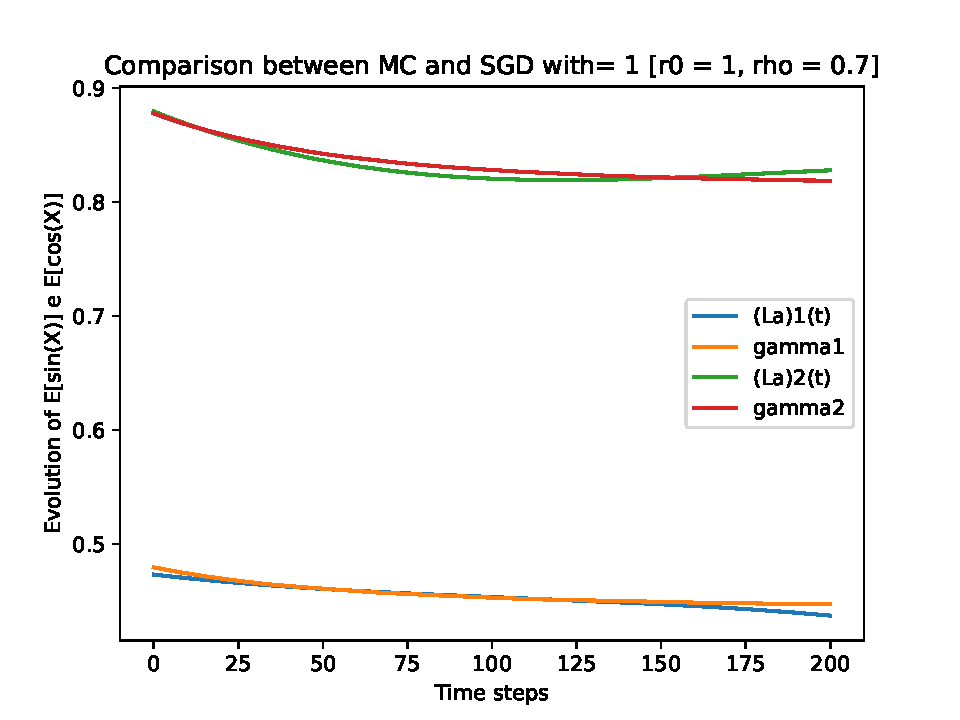
\includegraphics[width=0.9\textwidth]{images/graphics T = 2/n = 3, M = 1 sine and cosine.pdf}
\end{figure}
\begin{figure}[H]
\centering
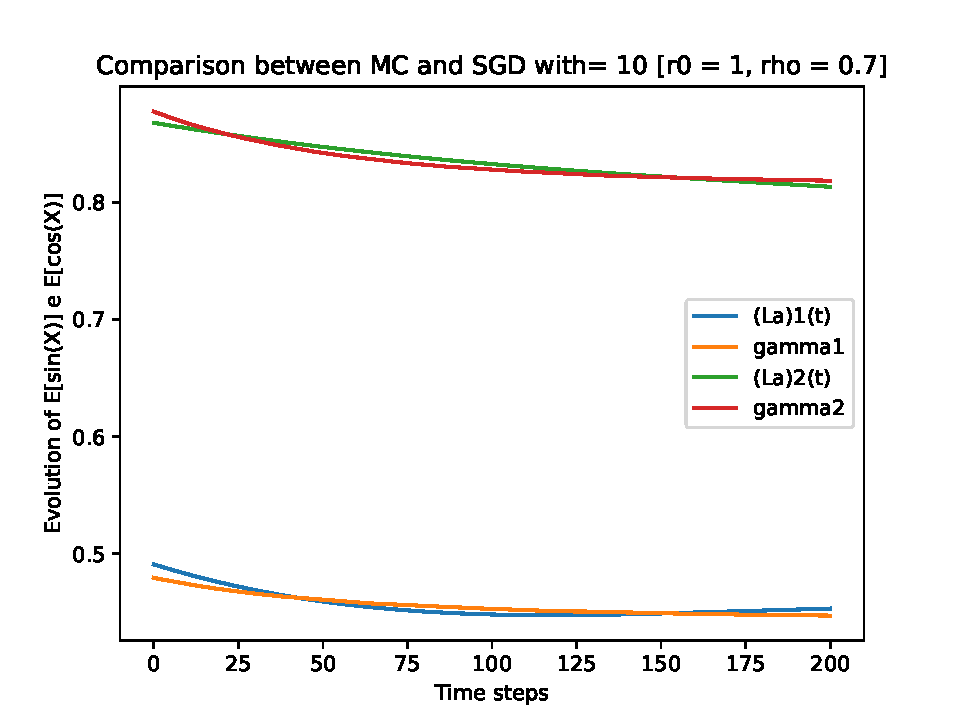
\includegraphics[width=0.9\textwidth]{images/graphics T = 2/n = 3, M = 10 sine and cosine.pdf}
\end{figure}
\begin{figure}[H]
\centering
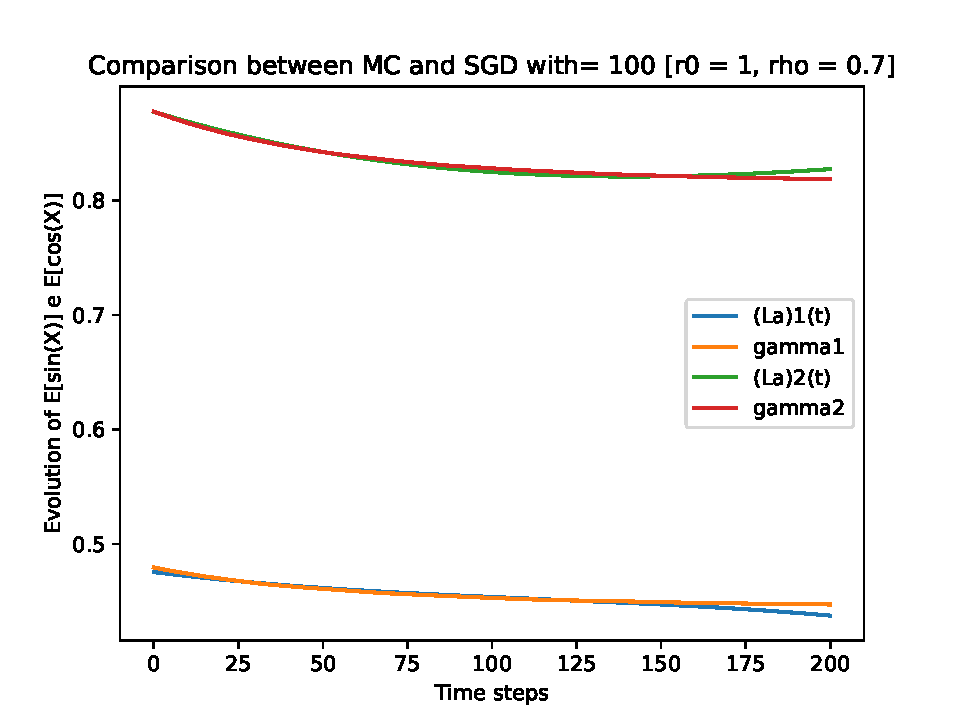
\includegraphics[width=0.9\textwidth]{images/graphics T = 2/n = 3, M = 100 sine and cosine.pdf}
\end{figure}
\begin{figure}[H]
\centering
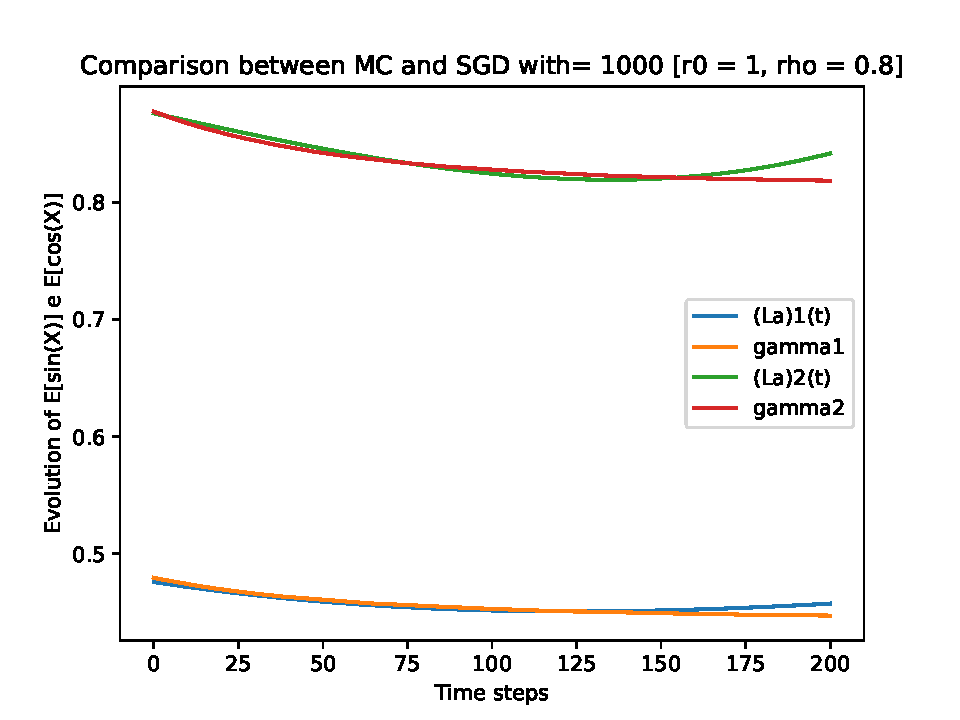
\includegraphics[width=0.9\textwidth]{images/graphics T = 2/n = 3, M = 1000 sine and cosine.pdf}
\end{figure}
\begin{figure}[H]
\centering
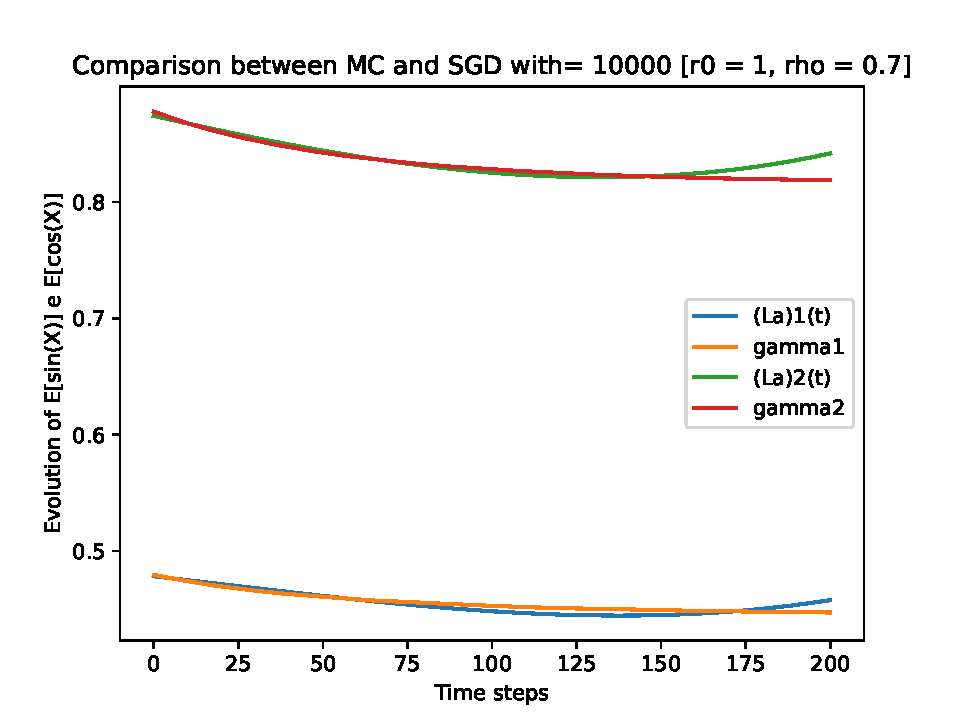
\includegraphics[width=0.9\textwidth]{images/graphics T = 2/n = 3, M = 10000 sine and cosine.pdf}
\end{figure}
\newpage
\section*{Caso n = 4} 
\begin{table}[H]
\centering
\addtolength{\leftskip}{-1.5cm}
\addtolength{\rightskip}{-1.5cm}
\begin{tabular}{|c|ll|}
\hline
$ $ & $r_0 = 1$ & $r_0 = 5$ \\
\hline
$\rho = 0.6$ & 29.67 & 104.08 \\

$\rho = 0.7$ & 19.5 & 58.47 \\

$\rho = 0.8$ & 44.65 & 23.28 \\

$\rho = 0.9$ & 271.35 & 17.65 \\
\hline
\end{tabular}
\caption{Average execution
 times (in seconds $s$) with $M = 1$}
\end{table}
\begin{table}[H]
\centering
\addtolength{\leftskip}{-1.5cm}
\addtolength{\rightskip}{-1.5cm}
\begin{tabular}{|c|lllllllll|}
\hline
$ $ & $r_0 = 1$ & $r_0 = 1$ & $r_0 = 1$ & $r_0 = 5$ & $r_0 = 5$ & $r_0 = 5$ & $r_0 = 10$ & $r_0 = 10$ & $r_0 = 10$  \\
$ $ & min & max & average & min & max & average & min & max & average \\ 
\hline
$\rho = 0.6$ & 620 & 4050 & 2331 & 2890 & 11970 & 7908 &  & overflow &  \\

$\rho = 0.7$ & 670 & 3850 & 1529 & 1570 & 6540 & 4510 &  & overflow &  \\

$\rho = 0.8$ & 490 & 13550 & 3428 & 280 & 4230 & 1806 &  & overflow & \\

$\rho = 0.9$ & 1560 & 49999 & 20370.8 & 670 & 2480 & 1312 &  & overflow & \\
\hline
\end{tabular}
\caption{Number of iterations $m$ to achieve convergence with $M = 1$}
\end{table}
\begin{table}[H]
\centering
\addtolength{\leftskip}{-1.5cm}
\addtolength{\rightskip}{-1.5cm}
\begin{tabular}{|c|ll|}
\hline
$ $ & $r_0 = 1$ & $r_0 = 5$ \\
\hline
$\rho = 0.6$ & 4.56 & 13.23  \\

$\rho = 0.7$ & 4.85 & 7.61  \\

$\rho = 0.8$ & 6.83 & 5.09  \\

$\rho = 0.9$ & 29.93 & 4.01  \\
\hline
\end{tabular}
\caption{Average execution
 times (in seconds $s$) with $M = 10$}
\end{table}
\begin{table}[H]
\centering
\addtolength{\leftskip}{-1.5cm}
\addtolength{\rightskip}{-1.5cm}
\begin{tabular}{|c|lllllllll|}
\hline
$ $ & $r_0 = 1$ & $r_0 = 1$ & $r_0 = 1$ & $r_0 = 5$ & $r_0 = 5$ & $r_0 = 5$ & $r_0 = 10$ & $r_0 = 10$ & $r_0 = 10$  \\
$ $ & min & max & average & min & max & average & min & max & average \\ 
\hline
$\rho = 0.6$ & 80 & 620 & 310 & 340 & 1380 & 886 &  & overflow &  \\

$\rho = 0.7$ & 20 & 810 & 322 & 290 & 1090 & 519 &  & overflow &  \\

$\rho = 0.8$ & 40 & 2420 & 438 & 80 & 680 & 348 &  & overflow & \\

$\rho = 0.9$ & 60 & 6660 & 1909 & 110 & 690 & 273 &  & overflow & \\
\hline
\end{tabular}
\caption{Number of iterations $m$ to achieve convergence with $M = 10$}
\end{table}
\begin{table}[H]
\centering
\addtolength{\leftskip}{-1.5cm}
\addtolength{\rightskip}{-1.5cm}
\begin{tabular}{|c|ll|}
\hline
$ $ & $r_0 = 1$ & $r_0 = 5$ \\
\hline
$\rho = 0.6$ & 0.84 & 2.54  \\

$\rho = 0.7$ & 1.13 & 1.82  \\

$\rho = 0.8$ & 1.41 & 1.38  \\

$\rho = 0.9$ & 4.74 & 1.27  \\
\hline
\end{tabular}
\caption{Average execution
 times (in seconds $s$) with $M = 100$}
\end{table}
\begin{table}[H]
\centering
\addtolength{\leftskip}{-1.5cm}
\addtolength{\rightskip}{-1.5cm}
\begin{tabular}{|c|lllllllll|}
\hline
$ $ & $r_0 = 1$ & $r_0 = 1$ & $r_0 = 1$ & $r_0 = 5$ & $r_0 = 5$ & $r_0 = 5$ & $r_0 = 10$ & $r_0 = 10$ & $r_0 = 10$  \\
$ $ & min & max & average & min & max & average & min & max & average \\ 
\hline
$\rho = 0.6$ & 10 & 90 & 31 & 30 & 190 & 90 &  & overflow &  \\

$\rho = 0.7$ & 10 & 110 & 40 & 30 & 100 & 64 &  & overflow &  \\

$\rho = 0.8$ & 10 & 150 & 42 & 30 & 70 & 49 &  & overflow & \\

$\rho = 0.9$ & 20 & 950 & 169 & 10 & 80 & 45 &  & overflow & \\
\hline
\end{tabular}
\caption{Number of iterations $m$ to achieve convergence with $M = 100$}
\end{table}
\begin{table}[H]
\centering
\addtolength{\leftskip}{-1.5cm}
\addtolength{\rightskip}{-1.5cm}
\begin{tabular}{|c|ll|}
\hline
$ $ & $r_0 = 1$ & $r_0 = 5$ \\
\hline
$\rho = 0.6$ & 1.43 & 3.93 \\

$\rho = 0.7$ & 1.27 & 3.09 \\

$\rho = 0.8$ & 1.34 & 2.35 \\

$\rho = 0.9$ & 1.92 & 2.17 \\
\hline
\end{tabular}
\caption{Average execution
 times (in seconds $s$) with $M = 1000$}
\end{table}
\begin{table}[H]
\centering
\addtolength{\leftskip}{-1.5cm}
\addtolength{\rightskip}{-1.5cm}
\begin{tabular}{|c|lllllllll|}
\hline
$ $ & $r_0 = 1$ & $r_0 = 1$ & $r_0 = 1$ & $r_0 = 5$ & $r_0 = 5$ & $r_0 = 5$ & $r_0 = 10$ & $r_0 = 10$ & $r_0 = 10$  \\
$ $ & min & max & average & min & max & average & min & max & average \\ 
\hline
$\rho = 0.6$ & 4 & 11 & 6 & 13 & 20 & 16.4 &  & overflow &  \\

$\rho = 0.7$ & 3 & 11 & 5.3 & 10 & 21 & 12.8 &  & overflow &  \\

$\rho = 0.8$ & 4 & 11 & 5.6 & 8 & 13 & 9.7 &  & overflow & \\

$\rho = 0.9$ & 4 & 23 & 8 & 7 & 14 & 9.1 &  &overflow  & \\
\hline
\end{tabular}
\caption{Number of iterations $m$ to achieve convergence with $M = 1000$}
\end{table}
\begin{table}[H]
\centering
\addtolength{\leftskip}{-1.5cm}
\addtolength{\rightskip}{-1.5cm}
\begin{tabular}{|c|ll|}
\hline
$ $ & $r_0 = 1$ & $r_0 = 5$  \\
\hline
$\rho = 0.6$ & 7.24 & 30.59 \\

$\rho = 0.7$ & 7.20 & 22.75 \\

$\rho = 0.8$ & 7.77 & 18.19 \\

$\rho = 0.9$ & 8.51 & 16.25 \\
\hline
\end{tabular}
\caption{Average execution
 times (in seconds $s$) with $M = 10000$}
\end{table}
\begin{table}[H]
\centering
\addtolength{\leftskip}{-1.5cm}
\addtolength{\rightskip}{-1.5cm}
\begin{tabular}{|c|lllllllll|}
\hline
$ $ & $r_0 = 1$ & $r_0 = 1$ & $r_0 = 1$ & $r_0 = 5$ & $r_0 = 5$ & $r_0 = 5$ & $r_0 = 10$ & $r_0 = 10$ & $r_0 = 10$  \\
$ $ & min & max & average & min & max & average & min & max & average \\ 
\hline
$\rho = 0.6$ & 3 & 4 & 3.1 & 13 & 13 & 13 &  & overflow &  \\

$\rho = 0.7$ & 3 & 4 & 3.1 & 10 & 10 & 10 &  & overflow &  \\

$\rho = 0.8$ & 3 & 4 & 3.3 & 8 & 8 & 8 &  & overflow & \\

$\rho = 0.9$ & 3 & 4 & 3.6 & 7 & 7 & 7 &  & overflow & \\
\hline
\end{tabular}
\caption{Number of iterations $m$ to achieve convergence with $M = 10000$}
\end{table}
\begin{figure}[H]
\centering
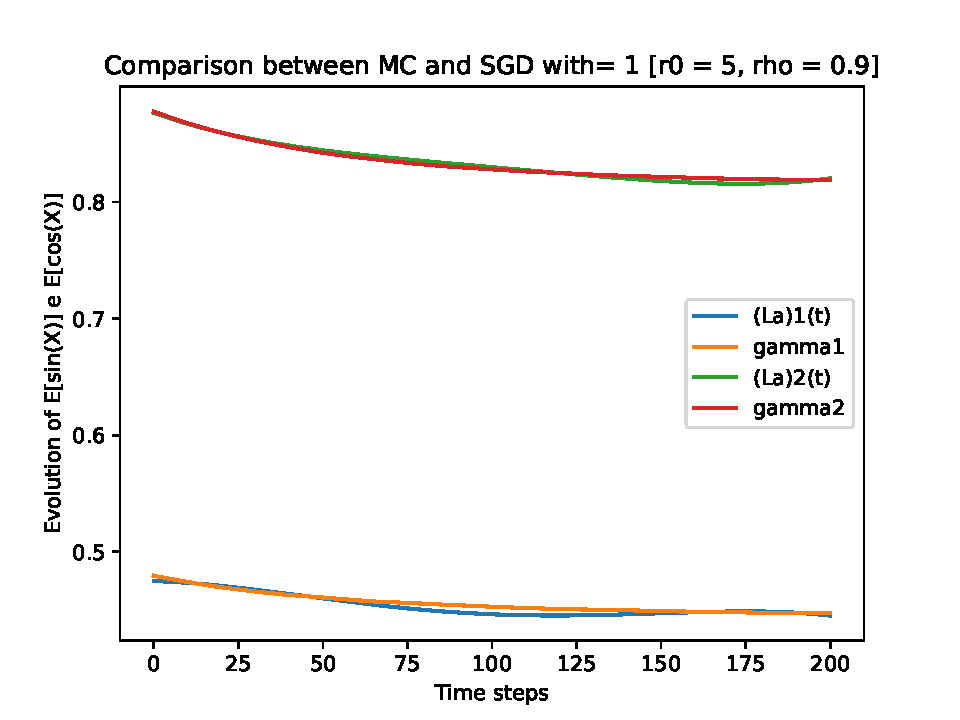
\includegraphics[width=0.9\textwidth]{images/graphics T = 2/n = 4, M = 1 sine and cosine.pdf}
\end{figure}
\begin{figure}[H]
\centering
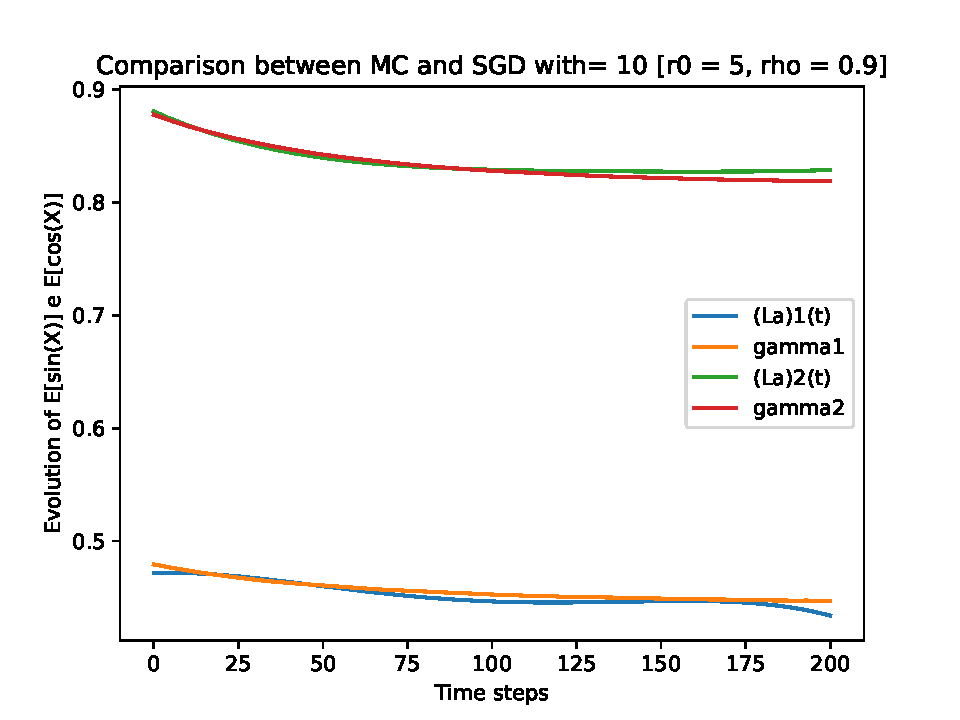
\includegraphics[width=0.9\textwidth]{images/graphics T = 2/n = 4, M = 10 sine and cosine.pdf}
\end{figure}
\begin{figure}[H]
\centering
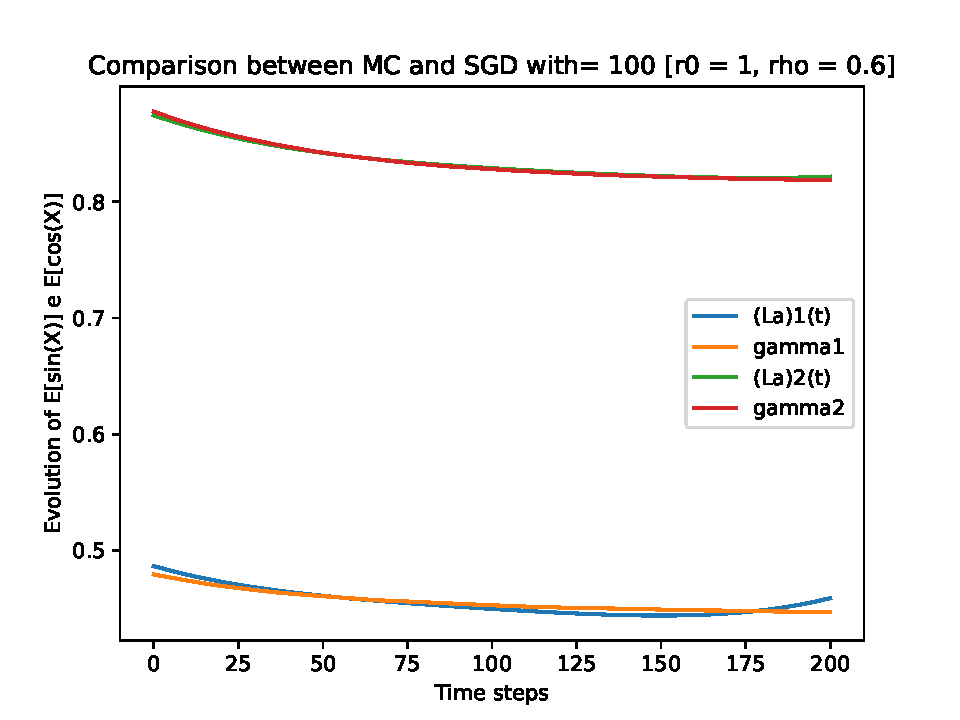
\includegraphics[width=0.9\textwidth]{images/graphics T = 2/n = 4, M = 100 sine and cosine.pdf}
\end{figure}
\begin{figure}[H]
\centering
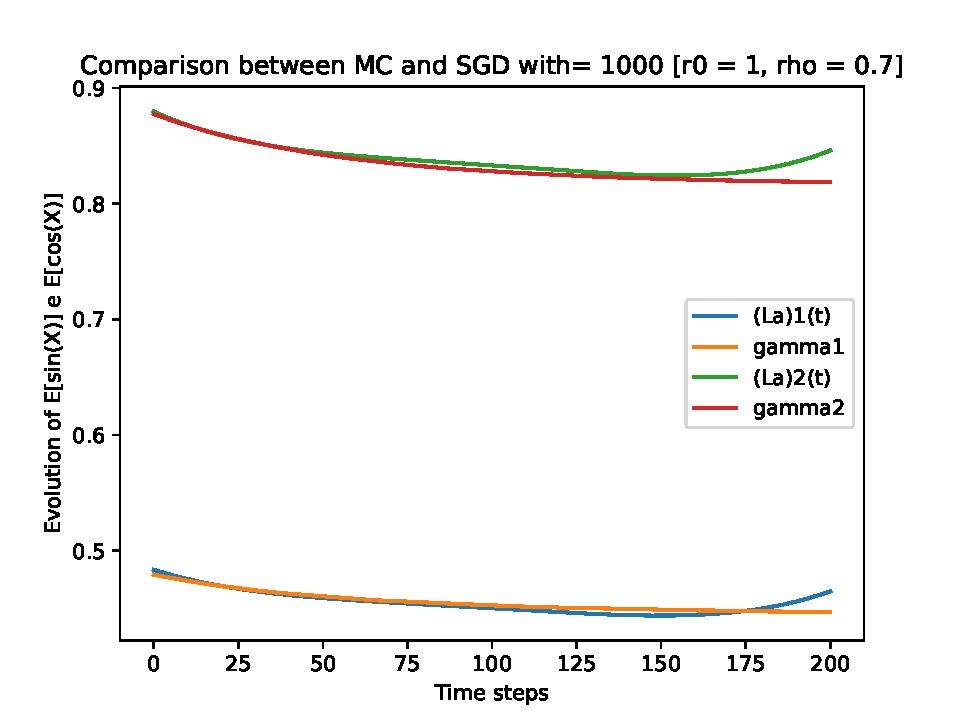
\includegraphics[width=0.9\textwidth]{images/graphics T = 2/n = 4, M = 1000 sine and cosine.pdf}
\end{figure}
\begin{figure}[H]
\centering
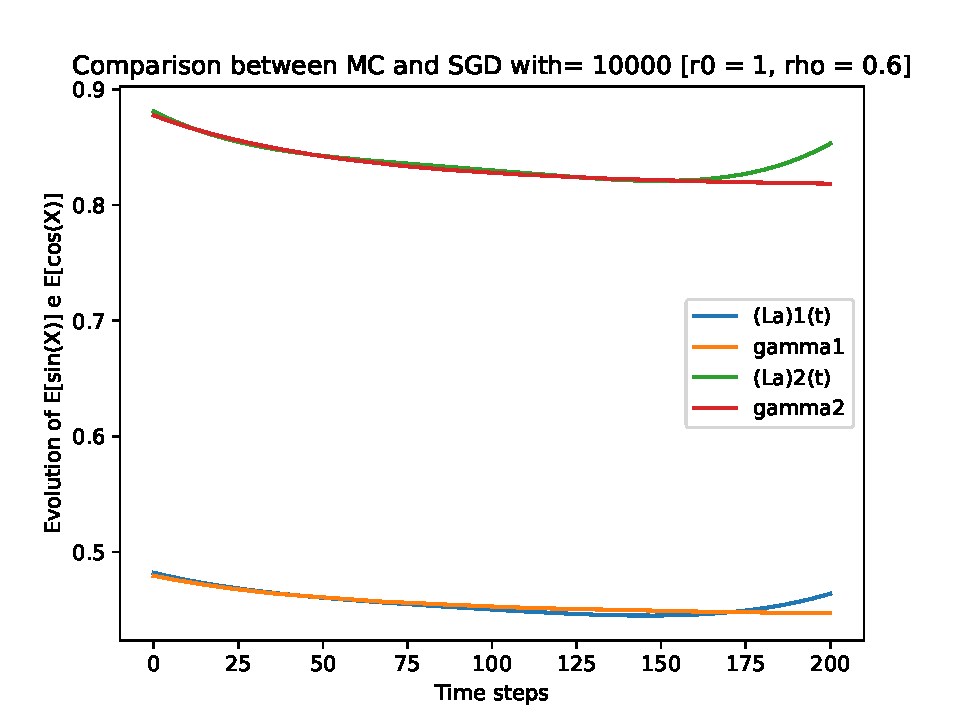
\includegraphics[width=0.9\textwidth]{images/graphics T = 2/n = 4, M = 10000 sine and cosine.pdf}
\end{figure}
\newpage
\section*{Caso n = 5} 
\begin{table}[H]
\centering
\addtolength{\leftskip}{-1.5cm}
\addtolength{\rightskip}{-1.5cm}
\begin{tabular}{|c|ll|}
\hline
$ $ & $r_0 = 1$ & $r_0 = 5$ \\
\hline
$\rho = 0.6$ & 28.57 & 133.75 \\

$\rho = 0.7$ & 33.20 & 54.61 \\

$\rho = 0.8$ & 59.02 & 42.73 \\

$\rho = 0.9$ &  306.42 & 20.43 \\
\hline
\end{tabular}
\caption{Average execution
 times (in seconds $s$) with $M = 1$}
\end{table}
\begin{table}[H]
\centering
\addtolength{\leftskip}{-1.5cm}
\addtolength{\rightskip}{-1.5cm}
\begin{tabular}{|c|lllllllll|}
\hline
$ $ & $r_0 = 1$ & $r_0 = 1$ & $r_0 = 1$ & $r_0 = 5$ & $r_0 = 5$ & $r_0 = 5$ & $r_0 = 10$ & $r_0 = 10$ & $r_0 = 10$  \\
$ $ & min & max & average & min & max & average & min & max & average \\ 
\hline
$\rho = 0.6$ & 820 & 3420 & 2167 & 4540 & 17080 & 10248 &  & overflow &  \\

$\rho = 0.7$ & 490 & 6630 & 2459 & 2280 & 8430 & 4194 &  & overflow &  \\

$\rho = 0.8$ & 470 & 9120 & 4432 & 1410 & 7030 & 3278 &  & overflow & \\

$\rho = 0.9$ & 1160 & 49999 & 23456.7 & 400 & 4680 & 1570 &  & overflow & \\
\hline
\end{tabular}
\caption{Number of iterations $m$ to achieve convergence with $M = 1$}
\end{table}
\begin{table}[H]
\centering
\addtolength{\leftskip}{-1.5cm}
\addtolength{\rightskip}{-1.5cm}
\begin{tabular}{|c|ll|}
\hline
$ $ & $r_0 = 1$ & $r_0 = 5$ \\
\hline
$\rho = 0.6$ & 4.13 & 13.39 \\

$\rho = 0.7$ & 5.30 & 7.85  \\

$\rho = 0.8$ & 18.94 & 3.82 \\

$\rho = 0.9$ & 53.15 & 5.07 \\
\hline
\end{tabular}
\caption{Average execution
 times (in seconds $s$) with $M = 10$}
\end{table}
\begin{table}[H]
\centering
\addtolength{\leftskip}{-1.5cm}
\addtolength{\rightskip}{-1.5cm}
\begin{tabular}{|c|lllllllll|}
\hline
$ $ & $r_0 = 1$ & $r_0 = 1$ & $r_0 = 1$ & $r_0 = 5$ & $r_0 = 5$ & $r_0 = 5$ & $r_0 = 10$ & $r_0 = 10$ & $r_0 = 10$  \\
$ $ & min & max & average & min & max & average & min & max & average \\ 
\hline
$\rho = 0.6$ & 90 & 490 & 272 & 380 & 1610 & 883 &  & overflow &  \\

$\rho = 0.7$ & 100 & 570 & 333 & 180 & 950 & 517 &  & overflow &  \\

$\rho = 0.8$ & 70 & 6300 & 1230 & 90 & 510 & 252 &  & overflow & \\

$\rho = 0.9$ & 80 & 24990 & 3503 & 150 & 1130 & 335 &  & overflow & \\
\hline
\end{tabular}
\caption{Number of iterations $m$ to achieve convergence with $M = 10$}
\end{table}
\begin{table}[H]
\centering
\addtolength{\leftskip}{-1.5cm}
\addtolength{\rightskip}{-1.5cm}
\begin{tabular}{|c|ll|}
\hline
$ $ & $r_0 = 1$ & $r_0 = 5$ \\
\hline
$\rho = 0.6$ & 1.99 & 2.05  \\

$\rho = 0.7$ & 1.05 & 2.14  \\

$\rho = 0.8$ & 1.84 & 2.11  \\

$\rho = 0.9$ & 3.72 & 1.92  \\
\hline
\end{tabular}
\caption{Average execution
 times (in seconds $s$) with $M = 100$}
\end{table}
\begin{table}[H]
\centering
\addtolength{\leftskip}{-1.5cm}
\addtolength{\rightskip}{-1.5cm}
\begin{tabular}{|c|lllllllll|}
\hline
$ $ & $r_0 = 1$ & $r_0 = 1$ & $r_0 = 1$ & $r_0 = 5$ & $r_0 = 5$ & $r_0 = 5$ & $r_0 = 10$ & $r_0 = 10$ & $r_0 = 10$  \\
$ $ & min & max & average & min & max & average & min & max & average \\ 
\hline
$\rho = 0.6$ & 20 & 190 & 68 & 40 & 130 & 70 &  & overflow &  \\

$\rho = 0.7$ & 10 & 80 & 36 & 20 & 170 & 73 &  & overflow &  \\

$\rho = 0.8$ & 10 & 180 & 63 & 30 & 150 & 72 &  & overflow & \\

$\rho = 0.9$ & 10 & 680 & 127 & 30 & 120 & 65 &  & overflow & \\
\hline
\end{tabular}
\caption{Number of iterations $m$ to achieve convergence with $M = 100$}
\end{table}
\begin{table}[H]
\centering
\addtolength{\leftskip}{-1.5cm}
\addtolength{\rightskip}{-1.5cm}
\begin{tabular}{|c|ll|}
\hline
$ $ & $r_0 = 1$ & $r_0 = 5$  \\
\hline
$\rho = 0.6$ & 1.59 & 3.27  \\

$\rho = 0.7$ & 1.98 & 2.5  \\

$\rho = 0.8$ & 1.86 & 2.56  \\

$\rho = 0.9$ & 2.85 & 1.93  \\
\hline
\end{tabular}
\caption{Average execution
 times (in seconds $s$) with $M = 1000$}
\end{table}
\begin{table}[H]
\centering
\addtolength{\leftskip}{-1.5cm}
\addtolength{\rightskip}{-1.5cm}
\begin{tabular}{|c|lllllllll|}
\hline
$ $ & $r_0 = 1$ & $r_0 = 1$ & $r_0 = 1$ & $r_0 = 5$ & $r_0 = 5$ & $r_0 = 5$ & $r_0 = 10$ & $r_0 = 10$ & $r_0 = 10$  \\
$ $ & min & max & average & min & max & average & min & max & average \\ 
\hline
$\rho = 0.6$ & 4 & 10 & 6.1 & 10 & 17 & 12.4 &  & overflow &  \\

$\rho = 0.7$ & 4 & 16 & 7.6 & 8 & 13 & 9.6 &  & overflow &  \\

$\rho = 0.8$ & 5 & 12 & 7.1 & 7 & 14 & 9.8 &  & overflow & \\

$\rho = 0.9$ & 7 & 18 & 11 & 5 & 12 & 7.4 &  & overflow & \\
\hline
\end{tabular}
\caption{Number of iterations $m$ to achieve convergence with $M = 1000$}
\end{table}
\begin{table}[H]
\centering
\addtolength{\leftskip}{-1.5cm}
\addtolength{\rightskip}{-1.5cm}
\begin{tabular}{|c|ll|}
\hline
$ $ & $r_0 = 1$ & $r_0 = 5$  \\
\hline
$\rho = 0.6$ & 10.72 & 26.45 \\

$\rho = 0.7$ & 11.51 & 21.05 \\

$\rho = 0.8$ & 15.16 & 15.97  \\

$\rho = 0.9$ & 16.24 & 13.36  \\
\hline
\end{tabular}
\caption{Average execution
 times (in seconds $s$) with $M = 10000$}
\end{table}
\begin{table}[H]
\centering
\addtolength{\leftskip}{-1.5cm}
\addtolength{\rightskip}{-1.5cm}
\begin{tabular}{|c|lllllllll|}
\hline
$ $ & $r_0 = 1$ & $r_0 = 1$ & $r_0 = 1$ & $r_0 = 5$ & $r_0 = 5$ & $r_0 = 5$ & $r_0 = 10$ & $r_0 = 10$ & $r_0 = 10$  \\
$ $ & min & max & average & min & max & average & min & max & average \\ 
\hline
$\rho = 0.6$ & 4 & 5 & 4.1 & 10 & 11 & 10.1 &  & overflow &  \\

$\rho = 0.7$ & 4 & 5 & 4.4 & 8 & 8 & 8 &  & overflow &  \\

$\rho = 0.8$ & 5 & 8 & 5.8 & 6 & 7 & 6.1 &  & overflow & \\

$\rho = 0.9$ & 5 & 8 & 6.2 & 5 & 6 & 5.1 &  & overflow & \\
\hline
\end{tabular}
\caption{Number of iterations $m$ to achieve convergence with $M = 10000$}
\end{table}
\begin{figure}[H]
\centering
\includegraphics[width=0.9\textwidth]{images/graphics T = 2/n = 5, M = 1 sine and cosine.pdf}
\end{figure}
\begin{figure}[H]
\centering
\includegraphics[width=0.9\textwidth]{images/graphics T = 2/n = 5, M = 10 sine and cosine.pdf}
\end{figure}
\begin{figure}[H]
\centering
\includegraphics[width=0.9\textwidth]{images/graphics T = 2/n = 5, M = 100 sine and cosine.pdf}
\end{figure}
\begin{figure}[H]
\centering
\includegraphics[width=0.9\textwidth]{images/graphics T = 2/n = 5, M = 1000 sine and cosine.pdf}
\end{figure}
\begin{figure}[H]
\centering
\includegraphics[width=0.9\textwidth]{images/graphics T = 2/n = 5, M = 10000 sine and cosine.pdf}
\end{figure}
\newpage
\section*{Caso n = 6} 
\begin{table}[H]
\centering
\addtolength{\leftskip}{-1.5cm}
\addtolength{\rightskip}{-1.5cm}
\begin{tabular}{|c|lll|}
\hline
$ $ & $r_0 = 1$ & $r_0 = 5$ & $r_0 = 10$ \\
\hline
$\rho = 0.6$ & 32.08 & 143.46 &  \\

$\rho = 0.7$ & 17.72 & 59.82 &  \\

$\rho = 0.8$ & 45.81 & 38.29 & 56.83 \\

$\rho = 0.9$ & 415.62 & 20.29 & 33.01 \\
\hline
\end{tabular}
\caption{Average execution
 times (in seconds $s$) with $M = 1$}
\end{table}
\begin{table}[H]
\centering
\addtolength{\leftskip}{-1.5cm}
\addtolength{\rightskip}{-1.5cm}
\begin{tabular}{|c|lllllllll|}
\hline
$ $ & $r_0 = 1$ & $r_0 = 1$ & $r_0 = 1$ & $r_0 = 5$ & $r_0 = 5$ & $r_0 = 5$ & $r_0 = 10$ & $r_0 = 10$ & $r_0 = 10$  \\
$ $ & min & max & average & min & max & average & min & max & average \\ 
\hline
$\rho = 0.6$ & 530 & 5630 & 2424 & 4710 & 21280 & 10855 &  & overflow &  \\

$\rho = 0.7$ & 380 & 3370 & 1336 & 990 & 8130 & 4511 &  & overflow &  \\

$\rho = 0.8$ & 900 & 12100 & 3456 & 1050 & 4840 & 2893 & 2490 & 6850 & 4171 \\

$\rho = 0.9$ & 7640 & 49999 & 31384.5 & 440 & 4390 & 1532 & 1620 & 4050 & 2405\\
\hline
\end{tabular}
\caption{Number of iterations $m$ to achieve convergence with $M = 1$}
\end{table}
\begin{table}[H]
\centering
\addtolength{\leftskip}{-1.5cm}
\addtolength{\rightskip}{-1.5cm}
\begin{tabular}{|c|lll|}
\hline
$ $ & $r_0 = 1$ & $r_0 = 5$ & $r_0 = 10$ \\
\hline
$\rho = 0.6$ & 3.39 & 14.24 &  \\

$\rho = 0.7$ & 5.58 & 6.85 &  \\

$\rho = 0.8$ & 19.75 & 7.34 & 8.91 \\

$\rho = 0.9$ & 15.37 & 5.23 & 5.81 \\
\hline
\end{tabular}
\caption{Average execution
 times (in seconds $s$) with $M = 10$}
\end{table}
\begin{table}[H]
\centering
\addtolength{\leftskip}{-1.5cm}
\addtolength{\rightskip}{-1.5cm}
\begin{tabular}{|c|lllllllll|}
\hline
$ $ & $r_0 = 1$ & $r_0 = 1$ & $r_0 = 1$ & $r_0 = 5$ & $r_0 = 5$ & $r_0 = 5$ & $r_0 = 10$ & $r_0 = 10$ & $r_0 = 10$  \\
$ $ & min & max & average & min & max & average & min & max & average \\ 
\hline
$\rho = 0.6$ & 50 & 640 & 219 & 410 & 1280 & 917 &  & overflow &  \\

$\rho = 0.7$ & 60 & 710 & 359 & 130 & 900 & 442 &  & overflow &  \\

$\rho = 0.8$ & 90 & 7070 & 1271 & 90 & 870 & 472 & 290 & 990 & 569 \\

$\rho = 0.9$ & 130 & 2720 & 988 & 70 & 670 & 337 & 100 & 750 & 369\\
\hline
\end{tabular}
\caption{Number of iterations $m$ to achieve convergence with $M = 10$}
\end{table}
\begin{table}[H]
\centering
\addtolength{\leftskip}{-1.5cm}
\addtolength{\rightskip}{-1.5cm}
\begin{tabular}{|c|lll|}
\hline
$ $ & $r_0 = 1$ & $r_0 = 5$ & $r_0 = 10$ \\
\hline
$\rho = 0.6$ & 1.07 & 3.43 &  \\

$\rho = 0.7$ & 0.80 & 2.40 &  \\

$\rho = 0.8$ & 3.97 & 2.23 & 4.02 \\

$\rho = 0.9$ & 9.14 & 1.61 & 2.75 \\
\hline
\end{tabular}
\caption{Average execution
 times (in seconds $s$) with $M = 100$}
\end{table}
\begin{table}[H]
\centering
\addtolength{\leftskip}{-1.5cm}
\addtolength{\rightskip}{-1.5cm}
\begin{tabular}{|c|lllllllll|}
\hline
$ $ & $r_0 = 1$ & $r_0 = 1$ & $r_0 = 1$ & $r_0 = 5$ & $r_0 = 5$ & $r_0 = 5$ & $r_0 = 10$ & $r_0 = 10$ & $r_0 = 10$  \\
$ $ & min & max & average & min & max & average & min & max & average \\ 
\hline
$\rho = 0.6$ & 10 & 50 & 35 & 60 & 170 & 111 &  & overflow &  \\

$\rho = 0.7$ & 10 & 60 & 26 & 40 & 160 & 78 &  & overflow &  \\

$\rho = 0.8$ & 10 & 520 & 129 & 30 & 190 & 72 & 70 & 260 & 127 \\

$\rho = 0.9$ & 20 & 1540 & 295 & 20 & 80 & 52 & 50 & 140 & 88\\
\hline
\end{tabular}
\caption{Number of iterations $m$ to achieve convergence with $M = 100$}
\end{table}
\begin{table}[H]
\centering
\addtolength{\leftskip}{-1.5cm}
\addtolength{\rightskip}{-1.5cm}
\begin{tabular}{|c|lll|}
\hline
$ $ & $r_0 = 1$ & $r_0 = 5$ & $r_0 = 10$ \\
\hline
$\rho = 0.6$ & 2.03 & 3.15 &  \\

$\rho = 0.7$ & 3.47 & 2.27 &  \\

$\rho = 0.8$ & 3.84 & 2.44 & 7.27 \\

$\rho = 0.9$ & 3.87 & 1.91 & 7.67 \\
\hline
\end{tabular}
\caption{Average execution
 times (in seconds $s$) with $M = 1000$}
\end{table}
\begin{table}[H]
\centering
\addtolength{\leftskip}{-1.5cm}
\addtolength{\rightskip}{-1.5cm}
\begin{tabular}{|c|lllllllll|}
\hline
$ $ & $r_0 = 1$ & $r_0 = 1$ & $r_0 = 1$ & $r_0 = 5$ & $r_0 = 5$ & $r_0 = 5$ & $r_0 = 10$ & $r_0 = 10$ & $r_0 = 10$  \\
$ $ & min & max & average & min & max & average & min & max & average \\ 
\hline
$\rho = 0.6$ & 5 & 10 & 6.8 & 8 & 24 & 10.7 &  & overflow &  \\

$\rho = 0.7$ & 6 & 32 & 11.8 & 6 & 12 & 7.7 &  & overflow &  \\

$\rho = 0.8$ & 7 & 29 & 13 & 5 & 15 & 8.3 & 20 & 31 & 23.4 \\

$\rho = 0.9$ & 8 & 32 & 13.1 & 5 & 10 & 6.5 & 13 & 50 & 24.7\\
\hline
\end{tabular}
\caption{Number of iterations $m$ to achieve convergence with $M = 1000$}
\end{table}
\begin{table}[H]
\centering
\addtolength{\leftskip}{-1.5cm}
\addtolength{\rightskip}{-1.5cm}
\begin{tabular}{|c|lll|}
\hline
$ $ & $r_0 = 1$ & $r_0 = 5$ & $r_0 = 10$ \\
\hline
$\rho = 0.6$ & 17.80 & 27.06 &  \\

$\rho = 0.7$ & 20.13 & 19.79 &  \\

$\rho = 0.8$ & 23.78 & 16.89 & 67.48 \\

$\rho = 0.9$ & 27.38 & 16.50 & 45.50 \\
\hline
\end{tabular}
\caption{Average execution
 times (in seconds $s$) with $M = 10000$}
\end{table}
\begin{table}[H]
\centering
\addtolength{\leftskip}{-1.5cm}
\addtolength{\rightskip}{-1.5cm}
\begin{tabular}{|c|lllllllll|}
\hline
$ $ & $r_0 = 1$ & $r_0 = 1$ & $r_0 = 1$ & $r_0 = 5$ & $r_0 = 5$ & $r_0 = 5$ & $r_0 = 10$ & $r_0 = 10$ & $r_0 = 10$  \\
$ $ & min & max & average & min & max & average & min & max & average \\ 
\hline
$\rho = 0.6$ & 5 & 7 & 5.4 & 8 & 9 & 8.2 &  & overflow &  \\

$\rho = 0.7$ & 6 & 7 & 6.1 & 6 & 6 & 6 &  & overflow &  \\

$\rho = 0.8$ & 7 & 8 & 7.2 & 5 & 6 & 5.1 & 17 & 24 & 18.8 \\

$\rho = 0.9$ & 7 & 9 & 8.3 & 5 & 5 & 5 & 12 & 17 & 13.6\\
\hline
\end{tabular}
\caption{Number of iterations $m$ to achieve convergence with $M = 10000$}
\end{table}
\begin{figure}[H]
\centering
\includegraphics[width=0.9\textwidth]{images/graphics T = 2/n = 6, M = 1 sine and cosine.pdf}
\end{figure}
\begin{figure}[H]
\centering
\includegraphics[width=0.9\textwidth]{images/graphics T = 2/n = 6, M = 10 sine and cosine.pdf}
\end{figure}
\begin{figure}[H]
\centering
\includegraphics[width=0.9\textwidth]{images/graphics T = 2/n = 6, M = 100 sine and cosine.pdf}
\end{figure}
\begin{figure}[H]
\centering
\includegraphics[width=0.9\textwidth]{images/graphics T = 2/n = 6, M = 1000 sine and cosine.pdf}
\end{figure}
\begin{figure}[H]
\centering
\includegraphics[width=0.9\textwidth]{images/graphics T = 2/n = 6, M = 10000 sine and cosine.pdf}
\end{figure}
\newpage
\section{T = 4}
\section*{Caso n = 3} 
\begin{table}[H]
\centering
\addtolength{\leftskip}{-1.5cm}
\addtolength{\rightskip}{-1.5cm}
\begin{tabular}{|c|l|}
\hline
$ $ & $r_0 = 1$ \\
\hline
$\rho = 0.6$ & 148.41 \\

$\rho = 0.7$ & 98.14 \\

$\rho = 0.8$ & 99.71 \\

$\rho = 0.9$ & 269.29 \\
\hline
\end{tabular}
\caption{Average execution
 times (in seconds $s$) with $M = 1$}
\end{table}
\begin{table}[H]
\centering
\addtolength{\leftskip}{-1.5cm}
\addtolength{\rightskip}{-1.5cm}
\begin{tabular}{|c|lllllllll|}
\hline
$ $ & $r_0 = 1$ & $r_0 = 1$ & $r_0 = 1$ & $r_0 = 5$ & $r_0 = 5$ & $r_0 = 5$ & $r_0 = 10$ & $r_0 = 10$ & $r_0 = 10$  \\
$ $ & min & max & average & min & max & average & min & max & average \\ 
\hline
$\rho = 0.6$ & 3450 & 12910 & 6042 &  & overflow &  &  & overflow &  \\

$\rho = 0.7$ & 1150 & 7610 & 3999 &  & overflow &  &  & overflow &  \\

$\rho = 0.8$ & 1030 & 9770 & 4062 &  & overflow &  &  & overflow & \\

$\rho = 0.9$ & 900 & 49999 & 10512.9 &  & overflow &  &  & overflow & \\
\hline
\end{tabular}
\caption{Number of iterations $m$ to achieve convergence with $M = 1$}
\end{table}
\begin{table}[H]
\centering
\addtolength{\leftskip}{-1.5cm}
\addtolength{\rightskip}{-1.5cm}
\begin{tabular}{|c|l|}
\hline
$ $ & $r_0 = 1$  \\
\hline
$\rho = 0.6$ & 15.35  \\

$\rho = 0.7$ & 10.90 \\

$\rho = 0.8$ & 8.20 \\

$\rho = 0.9$ & 72.03 \\
\hline
\end{tabular}
\caption{Average execution
 times (in seconds $s$) with $M = 10$}
\end{table}
\begin{table}[H]
\centering
\addtolength{\leftskip}{-1.5cm}
\addtolength{\rightskip}{-1.5cm}
\begin{tabular}{|c|lllllllll|}
\hline
$ $ & $r_0 = 1$ & $r_0 = 1$ & $r_0 = 1$ & $r_0 = 5$ & $r_0 = 5$ & $r_0 = 5$ & $r_0 = 10$ & $r_0 = 10$ & $r_0 = 10$  \\
$ $ & min & max & average & min & max & average & min & max & average \\ 
\hline
$\rho = 0.6$ & 170 & 1180 & 521 &  & overflow &  &  & overflow &  \\

$\rho = 0.7$ & 110 & 740 & 370 &  & overflow &  &  & overflow &  \\

$\rho = 0.8$ & 110 & 690 & 280 &  & overflow &  &  & overflow & \\

$\rho = 0.9$ & 50 & 12920 & 2475 &  & overflow &  &  & overflow & \\
\hline
\end{tabular}
\caption{Number of iterations $m$ to achieve convergence with $M = 10$}
\end{table}
\begin{table}[H]
\centering
\addtolength{\leftskip}{-1.5cm}
\addtolength{\rightskip}{-1.5cm}
\begin{tabular}{|c|l|}
\hline
$ $ & $r_0 = 1$  \\
\hline
$\rho = 0.6$ & 3.48 \\

$\rho = 0.7$ & 5.24 \\

$\rho = 0.8$ & 5.58  \\

$\rho = 0.9$ & 15.62 \\
\hline
\end{tabular}
\caption{Average execution
 times (in seconds $s$) with $M = 100$}
\end{table}
\begin{table}[H]
\centering
\addtolength{\leftskip}{-1.5cm}
\addtolength{\rightskip}{-1.5cm}
\begin{tabular}{|c|lllllllll|}
\hline
$ $ & $r_0 = 1$ & $r_0 = 1$ & $r_0 = 1$ & $r_0 = 5$ & $r_0 = 5$ & $r_0 = 5$ & $r_0 = 10$ & $r_0 = 10$ & $r_0 = 10$  \\
$ $ & min & max & average & min & max & average & min & max & average \\ 
\hline
$\rho = 0.6$ & 30 & 140 & 68 &  & overflow &  &  & overflow &  \\

$\rho = 0.7$ & 20 & 310 & 101 &  & overflow &  &  & overflow &  \\

$\rho = 0.8$ & 30 & 330 & 108 &  & overflow &  &  & overflow & \\

$\rho = 0.9$ & 20 & 1360 & 307 &  & overflow &  &  & overflow & \\
\hline
\end{tabular}
\caption{Number of iterations $m$ to achieve convergence with $M = 100$}
\end{table}
\begin{table}[H]
\centering
\addtolength{\leftskip}{-1.5cm}
\addtolength{\rightskip}{-1.5cm}
\begin{tabular}{|c|l|}
\hline
$ $ & $r_0 = 1$  \\
\hline
$\rho = 0.6$ & 2.06  \\

$\rho = 0.7$ & 3.32  \\

$\rho = 0.8$ & 3.08  \\

$\rho = 0.9$ & 2.61  \\
\hline
\end{tabular}
\caption{Average execution
 times (in seconds $s$) with $M = 1000$}
\end{table}
\begin{table}[H]
\centering
\addtolength{\leftskip}{-1.5cm}
\addtolength{\rightskip}{-1.5cm}
\begin{tabular}{|c|lllllllll|}
\hline
$ $ & $r_0 = 1$ & $r_0 = 1$ & $r_0 = 1$ & $r_0 = 5$ & $r_0 = 5$ & $r_0 = 5$ & $r_0 = 10$ & $r_0 = 10$ & $r_0 = 10$  \\
$ $ & min & max & average & min & max & average & min & max & average \\ 
\hline
$\rho = 0.6$ & 4 & 8 & 4.7 &  & overflow &  &  & overflow &  \\

$\rho = 0.7$ & 4 & 16 & 7.8 &  & overflow &  &  & overflow &  \\

$\rho = 0.8$ & 3 & 19 & 7.1 &  & overflow &  &  & overflow & \\

$\rho = 0.9$ & 4 & 9 & 6 &  & overflow &  &  & overflow & \\
\hline
\end{tabular}
\caption{Number of iterations $m$ to achieve convergence with $M = 1000$}
\end{table}
\begin{table}[H]
\centering
\addtolength{\leftskip}{-1.5cm}
\addtolength{\rightskip}{-1.5cm}
\begin{tabular}{|c|l|}
\hline
$ $ & $r_0 = 1$   \\
\hline
$\rho = 0.6$ & 16.91  \\

$\rho = 0.7$ & 16.04  \\

$\rho = 0.8$ & 12.17  \\

$\rho = 0.9$ & 12.15  \\
\hline
\end{tabular}
\caption{Average execution
 times (in seconds $s$) with $M = 10000$}
\end{table}
\begin{table}[H]
\centering
\addtolength{\leftskip}{-1.5cm}
\addtolength{\rightskip}{-1.5cm}
\begin{tabular}{|c|lllllllll|}
\hline
$ $ & $r_0 = 1$ & $r_0 = 1$ & $r_0 = 1$ & $r_0 = 5$ & $r_0 = 5$ & $r_0 = 5$ & $r_0 = 10$ & $r_0 = 10$ & $r_0 = 10$  \\
$ $ & min & max & average & min & max & average & min & max & average \\ 
\hline
$\rho = 0.6$ & 4 & 4 & 4 &  & overflow &  &  & overflow &  \\

$\rho = 0.7$ & 4 & 4 & 4 &  & overflow &  &  & overflow &  \\

$\rho = 0.8$ & 3 & 3 & 3 &  & overflow &  &  & overflow & \\

$\rho = 0.9$ & 3 & 3 & 3 &  & overflow &  &  & overflow & \\
\hline
\end{tabular}
\caption{Number of iterations $m$ to achieve convergence with $M = 10000$}
\end{table}
\begin{figure}[H]
\centering
\includegraphics[width=0.9\textwidth]{images/graphics T = 4/n = 3, M = 1 sine and cosine.pdf}
\end{figure}
\begin{figure}[H]
\centering
\includegraphics[width=0.9\textwidth]{images/graphics T = 4/n = 3, M = 10 sine and cosine.pdf}
\end{figure}
\begin{figure}[H]
\centering
\includegraphics[width=0.9\textwidth]{images/graphics T = 4/n = 3, M = 100 sine and cosine.pdf}
\end{figure}
\begin{figure}[H]
\centering
\includegraphics[width=0.9\textwidth]{images/graphics T = 4/n = 3, M = 1000 sine and cosine.pdf}
\end{figure}
\begin{figure}[H]
\centering
\includegraphics[width=0.9\textwidth]{images/graphics T = 4/n = 3, M = 10000 sine and cosine.pdf}
\end{figure}
\newpage
\section*{Caso n = 4} 
\begin{table}[H]
\centering
\addtolength{\leftskip}{-1.5cm}
\addtolength{\rightskip}{-1.5cm}
\begin{tabular}{|c|l|}
\hline
$ $ & $r_0 = 1$  \\
\hline
$\rho = 0.6$ & 145.11 \\

$\rho = 0.7$ & 102.23 \\

$\rho = 0.8$ & 177.10 \\

$\rho = 0.9$ & 890.75 \\
\hline
\end{tabular}
\caption{Average execution
 times (in seconds $s$) with $M = 1$}
\end{table}
\begin{table}[H]
\centering
\addtolength{\leftskip}{-1.5cm}
\addtolength{\rightskip}{-1.5cm}
\begin{tabular}{|c|lllllllll|}
\hline
$ $ & $r_0 = 1$ & $r_0 = 1$ & $r_0 = 1$ & $r_0 = 5$ & $r_0 = 5$ & $r_0 = 5$ & $r_0 = 10$ & $r_0 = 10$ & $r_0 = 10$  \\
$ $ & min & max & average & min & max & average & min & max & average \\ 
\hline
$\rho = 0.6$ & 3320 & 11980 & 5645 &  & overflow & &  & overflow &  \\

$\rho = 0.7$ & 1020 & 12700 & 3974 &  & overflow & &  & overflow &  \\

$\rho = 0.8$ & 740 & 25910 & 6650 &  & overflow & &  & overflow &  \\

$\rho = 0.9$ & 2470 & 49999 & 34868.5 &  & overflow & &  & overflow &  \\
\hline
\end{tabular}
\caption{Number of iterations $m$ to achieve convergence with $M = 1$}
\end{table}
\begin{table}[H]
\centering
\addtolength{\leftskip}{-1.5cm}
\addtolength{\rightskip}{-1.5cm}
\begin{tabular}{|c|l|}
\hline
$ $ & $r_0 = 1$  \\
\hline
$\rho = 0.6$ &  13.09 \\

$\rho = 0.7$ &  13.76 \\

$\rho = 0.8$ &  22.88 \\

$\rho = 0.9$ &  313.63 \\
\hline
\end{tabular}
\caption{Average execution
 times (in seconds $s$) with $M = 10$}
\end{table}
\begin{table}[H]
\centering
\addtolength{\leftskip}{-1.5cm}
\addtolength{\rightskip}{-1.5cm}
\begin{tabular}{|c|lllllllll|}
\hline
$ $ & $r_0 = 1$ & $r_0 = 1$ & $r_0 = 1$ & $r_0 = 5$ & $r_0 = 5$ & $r_0 = 5$ & $r_0 = 10$ & $r_0 = 10$ & $r_0 = 10$  \\
$ $ & min & max & average & min & max & average & min & max & average \\ 
\hline
$\rho = 0.6$ & 120 & 820 & 446 &  & overflow & &  & overflow &  \\

$\rho = 0.7$ & 250 & 820 & 473 &  & overflow & &  & overflow &  \\

$\rho = 0.8$ & 70 & 4380 & 778 &  & overflow & &  & overflow &  \\

$\rho = 0.9$ & 170 & 34500 & 10453 &  & overflow & &  & overflow &  \\
\hline
\end{tabular}
\caption{Number of iterations $m$ to achieve convergence with $M = 10$}
\end{table}
\begin{table}[H]
\centering
\addtolength{\leftskip}{-1.5cm}
\addtolength{\rightskip}{-1.5cm}
\begin{tabular}{|c|l|}
\hline
$ $ & $r_0 = 1$  \\
\hline
$\rho = 0.6$ & 4.71  \\

$\rho = 0.7$ & 2.61 \\

$\rho = 0.8$ & 5.88 \\

$\rho = 0.9$ & 37.38  \\
\hline
\end{tabular}
\caption{Average execution
 times (in seconds $s$) with $M = 100$}
\end{table}
\begin{table}[H]
\centering
\addtolength{\leftskip}{-1.5cm}
\addtolength{\rightskip}{-1.5cm}
\begin{tabular}{|c|lllllllll|}
\hline
$ $ & $r_0 = 1$ & $r_0 = 1$ & $r_0 = 1$ & $r_0 = 5$ & $r_0 = 5$ & $r_0 = 5$ & $r_0 = 10$ & $r_0 = 10$ & $r_0 = 10$  \\
$ $ & min & max & average & min & max & average & min & max & average \\ 
\hline
$\rho = 0.6$ & 40 & 160 & 88 &  & overflow & &  & overflow &  \\

$\rho = 0.7$ & 30 & 90 & 49 &  & overflow & &  & overflow &  \\

$\rho = 0.8$ & 10 & 390 & 108 &  & overflow & &  & overflow &  \\

$\rho = 0.9$ & 10 & 2810 & 703 &  & overflow & &  & overflow &  \\
\hline
\end{tabular}
\caption{Number of iterations $m$ to achieve convergence with $M = 100$}
\end{table}
\begin{table}[H]
\centering
\addtolength{\leftskip}{-1.5cm}
\addtolength{\rightskip}{-1.5cm}
\begin{tabular}{|c|l|}
\hline
$ $ & $r_0 = 1$  \\
\hline
$\rho = 0.6$ & 4.57 \\

$\rho = 0.7$ & 3.25 \\

$\rho = 0.8$ & 3.55 \\

$\rho = 0.9$ & 4.56 \\
\hline
\end{tabular}
\caption{Average execution
 times (in seconds $s$) with $M = 1000$}
\end{table}
\begin{table}[H]
\centering
\addtolength{\leftskip}{-1.5cm}
\addtolength{\rightskip}{-1.5cm}
\begin{tabular}{|c|lllllllll|}
\hline
$ $ & $r_0 = 1$ & $r_0 = 1$ & $r_0 = 1$ & $r_0 = 5$ & $r_0 = 5$ & $r_0 = 5$ & $r_0 = 10$ & $r_0 = 10$ & $r_0 = 10$  \\
$ $ & min & max & average & min & max & average & min & max & average \\ 
\hline
$\rho = 0.6$ & 4 & 18 & 9.5 &  & overflow & &  & overflow &  \\

$\rho = 0.7$ & 3 & 27 & 6.7 &  & overflow & &  & overflow &  \\

$\rho = 0.8$ & 3 & 18 & 7.4 &  & overflow & &  & overflow &  \\

$\rho = 0.9$ & 3 & 41 & 9.5 &  & overflow & &  & overflow &  \\
\hline
\end{tabular}
\caption{Number of iterations $m$ to achieve convergence with $M = 1000$}
\end{table}
\begin{table}[H]
\centering
\addtolength{\leftskip}{-1.5cm}
\addtolength{\rightskip}{-1.5cm}
\begin{tabular}{|c|l|}
\hline
$ $ & $r_0 = 1$  \\
\hline
$\rho = 0.6$ & 14.42 \\

$\rho = 0.7$ & 14.35 \\

$\rho = 0.8$ & 14.42 \\

$\rho = 0.9$ & 14.42 \\
\hline
\end{tabular}
\caption{Average execution
 times (in seconds $s$) with $M = 10000$}
\end{table}
\begin{table}[H]
\centering
\addtolength{\leftskip}{-1.5cm}
\addtolength{\rightskip}{-1.5cm}
\begin{tabular}{|c|lllllllll|}
\hline
$ $ & $r_0 = 1$ & $r_0 = 1$ & $r_0 = 1$ & $r_0 = 5$ & $r_0 = 5$ & $r_0 = 5$ & $r_0 = 10$ & $r_0 = 10$ & $r_0 = 10$  \\
$ $ & min & max & average & min & max & average & min & max & average \\ 
\hline
$\rho = 0.6$ & 3 & 3 & 3 &  & overflow & &  & overflow &  \\

$\rho = 0.7$ & 3 & 3 & 3 &  & overflow & &  & overflow &  \\

$\rho = 0.8$ & 3 & 3 & 3 &  & overflow & &  & overflow &  \\

$\rho = 0.9$ & 3 & 3 & 3 &  & overflow & &  & overflow &  \\
\hline
\end{tabular}
\caption{Number of iterations $m$ to achieve convergence with $M = 10000$}
\end{table}
\begin{figure}[H]
\centering
\includegraphics[width=0.9\textwidth]{images/graphics T = 4/n = 4, M = 1 sine and cosine.pdf}
\end{figure}
\begin{figure}[H]
\centering
\includegraphics[width=0.9\textwidth]{images/graphics T = 4/n = 4, M = 10 sine and cosine.pdf}
\end{figure}
\begin{figure}[H]
\centering
\includegraphics[width=0.9\textwidth]{images/graphics T = 4/n = 4, M = 100 sine and cosine.pdf}
\end{figure}
\begin{figure}[H]
\centering
\includegraphics[width=0.9\textwidth]{images/graphics T = 4/n = 4, M = 1000 sine and cosine.pdf}
\end{figure}
\begin{figure}[H]
\centering
\includegraphics[width=0.9\textwidth]{images/graphics T = 4/n = 4, M = 10000 sine and cosine.pdf}
\end{figure}
\newpage
\section*{Caso n = 5} 
\begin{table}[H]
\centering
\addtolength{\leftskip}{-1.5cm}
\addtolength{\rightskip}{-1.5cm}
\begin{tabular}{|c|l|}
\hline
$ $ & $r_0 = 1$ \\
\hline
$\rho = 0.6$ & 187.19 \\

$\rho = 0.7$ & 100.55 \\

$\rho = 0.8$ & 343.00 \\

$\rho = 0.9$ & 1090.67 \\
\hline
\end{tabular}
\caption{Average execution
 times (in seconds $s$) with $M = 1$}
\end{table}
\begin{table}[H]
\centering
\addtolength{\leftskip}{-1.5cm}
\addtolength{\rightskip}{-1.5cm}
\begin{tabular}{|c|lllllllll|}
\hline
$ $ & $r_0 = 1$ & $r_0 = 1$ & $r_0 = 1$ & $r_0 = 5$ & $r_0 = 5$ & $r_0 = 5$ & $r_0 = 10$ & $r_0 = 10$ & $r_0 = 10$  \\
$ $ & min & max & average & min & max & average & min & max & average \\ 
\hline
$\rho = 0.6$ & 2410 & 17200 & 7261 &  & overflow &  &  & overflow &  \\

$\rho = 0.7$ & 1490 & 6980 & 3871 &  & overflow &  &  & overflow &  \\

$\rho = 0.8$ & 640 & 42740 & 13311 &  & overflow &  &  & overflow & \\

$\rho = 0.9$ & 2840 & 49999 & 41910.3 &  & overflow &  &  & overflow & \\
\hline
\end{tabular}
\caption{Number of iterations $m$ to achieve convergence with $M = 1$}
\end{table}
\begin{table}[H]
\centering
\addtolength{\leftskip}{-1.5cm}
\addtolength{\rightskip}{-1.5cm}
\begin{tabular}{|c|l|}
\hline
$ $ & $r_0 = 1$  \\
\hline
$\rho = 0.6$ & 30.49  \\

$\rho = 0.7$ & 13.62  \\

$\rho = 0.8$ & 22.37  \\

$\rho = 0.9$ & 423.87   \\
\hline
\end{tabular}
\caption{Average execution
 times (in seconds $s$) with $M = 10$}
\end{table}
\begin{table}[H]
\centering
\addtolength{\leftskip}{-1.5cm}
\addtolength{\rightskip}{-1.5cm}
\begin{tabular}{|c|lllllllll|}
\hline
$ $ & $r_0 = 1$ & $r_0 = 1$ & $r_0 = 1$ & $r_0 = 5$ & $r_0 = 5$ & $r_0 = 5$ & $r_0 = 10$ & $r_0 = 10$ & $r_0 = 10$  \\
$ $ & min & max & average & min & max & average & min & max & average \\ 
\hline
$\rho = 0.6$ & 120 & 3880 & 1020 &  & overflow &  &  & overflow &  \\

$\rho = 0.7$ & 180 & 860 & 455 &  & overflow &  &  & overflow &  \\

$\rho = 0.8$ & 120 & 2540 & 743 &  & overflow &  &  & overflow & \\

$\rho = 0.9$ & 190 & 38600 & 14211 &  & overflow &  &  & overflow & \\
\hline
\end{tabular}
\caption{Number of iterations $m$ to achieve convergence with $M = 10$}
\end{table}
\begin{table}[H]
\centering
\addtolength{\leftskip}{-1.5cm}
\addtolength{\rightskip}{-1.5cm}
\begin{tabular}{|c|l|}
\hline
$ $ & $r_0 = 1$  \\
\hline
$\rho = 0.6$ & 3.98  \\

$\rho = 0.7$ & 3.58  \\

$\rho = 0.8$ & 13.71  \\

$\rho = 0.9$ & 108.12   \\
\hline
\end{tabular}
\caption{Average execution
 times (in seconds $s$) with $M = 100$}
\end{table}
\begin{table}[H]
\centering
\addtolength{\leftskip}{-1.5cm}
\addtolength{\rightskip}{-1.5cm}
\begin{tabular}{|c|lllllllll|}
\hline
$ $ & $r_0 = 1$ & $r_0 = 1$ & $r_0 = 1$ & $r_0 = 5$ & $r_0 = 5$ & $r_0 = 5$ & $r_0 = 10$ & $r_0 = 10$ & $r_0 = 10$  \\
$ $ & min & max & average & min & max & average & min & max & average \\ 
\hline
$\rho = 0.6$ & 30 & 150 & 68 &  & overflow &  &  & overflow &  \\

$\rho = 0.7$ & 20 & 100 & 61 &  & overflow &  &  & overflow &  \\

$\rho = 0.8$ & 40 & 910 & 234 &  & overflow &  &  & overflow & \\

$\rho = 0.9$ & 10 & 12040 & 1843 &  & overflow &  &  & overflow & \\
\hline
\end{tabular}
\caption{Number of iterations $m$ to achieve convergence with $M = 100$}
\end{table}
\begin{table}[H]
\centering
\addtolength{\leftskip}{-1.5cm}
\addtolength{\rightskip}{-1.5cm}
\begin{tabular}{|c|l|}
\hline
$ $ & $r_0 = 1$   \\
\hline
$\rho = 0.6$ & 4.24 \\

$\rho = 0.7$ & 7.74 \\

$\rho = 0.8$ & 2.61 \\

$\rho = 0.9$ & 2.29 \\
\hline
\end{tabular}
\caption{Average execution
 times (in seconds $s$) with $M = 1000$}
\end{table}
\begin{table}[H]
\centering
\addtolength{\leftskip}{-1.5cm}
\addtolength{\rightskip}{-1.5cm}
\begin{tabular}{|c|lllllllll|}
\hline
$ $ & $r_0 = 1$ & $r_0 = 1$ & $r_0 = 1$ & $r_0 = 5$ & $r_0 = 5$ & $r_0 = 5$ & $r_0 = 10$ & $r_0 = 10$ & $r_0 = 10$  \\
$ $ & min & max & average & min & max & average & min & max & average \\ 
\hline
$\rho = 0.6$ & 3 & 14 & 7.8 &  & overflow &  &  & overflow &  \\

$\rho = 0.7$ & 3 & 58 & 14.2 &  & overflow &  &  & overflow &  \\

$\rho = 0.8$ & 3 & 7 & 4.8 &  & overflow &  &  & overflow & \\

$\rho = 0.9$ & 2 & 6 & 4.2 &  & overflow &  &  & overflow & \\
\hline
\end{tabular}
\caption{Number of iterations $m$ to achieve convergence with $M = 1000$}
\end{table}
\begin{table}[H]
\centering
\addtolength{\leftskip}{-1.5cm}
\addtolength{\rightskip}{-1.5cm}
\begin{tabular}{|c|l|}
\hline
$ $ & $r_0 = 1$   \\
\hline
$\rho = 0.6$ & 15.91 \\

$\rho = 0.7$ & 12.07 \\

$\rho = 0.8$ & 11.51 \\

$\rho = 0.9$ & 13.16 \\
\hline
\end{tabular}
\caption{Average execution
 times (in seconds $s$) with $M = 10000$}
\end{table}
\begin{table}[H]
\centering
\addtolength{\leftskip}{-1.5cm}
\addtolength{\rightskip}{-1.5cm}
\begin{tabular}{|c|lllllllll|}
\hline
$ $ & $r_0 = 1$ & $r_0 = 1$ & $r_0 = 1$ & $r_0 = 5$ & $r_0 = 5$ & $r_0 = 5$ & $r_0 = 10$ & $r_0 = 10$ & $r_0 = 10$  \\
$ $ & min & max & average & min & max & average & min & max & average \\ 
\hline
$\rho = 0.6$ & 2 & 3 & 2.9 &  & overflow &  &  & overflow &  \\

$\rho = 0.7$ & 2 & 3 & 2.2 &  & overflow &  &  & overflow &  \\

$\rho = 0.8$ & 2 & 3 & 2.1 &  & overflow &  &  & overflow & \\

$\rho = 0.9$ & 2 & 3 & 2.4 &  & overflow &  &  & overflow & \\
\hline
\end{tabular}
\caption{Number of iterations $m$ to achieve convergence with $M = 10000$}
\end{table}
\begin{figure}[H]
\centering
\includegraphics[width=0.9\textwidth]{images/graphics T = 4/n = 5, M = 1 sine and cosine.pdf}
\end{figure}
\begin{figure}[H]
\centering
\includegraphics[width=0.9\textwidth]{images/graphics T = 4/n = 5, M = 10 sine and cosine.pdf}
\end{figure}
\begin{figure}[H]
\centering
\includegraphics[width=0.9\textwidth]{images/graphics T = 4/n = 5, M = 100 sine and cosine.pdf}
\end{figure}
\begin{figure}[H]
\centering
\includegraphics[width=0.9\textwidth]{images/graphics T = 4/n = 5, M = 1000 sine and cosine.pdf}
\end{figure}
\begin{figure}[H]
\centering
\includegraphics[width=0.9\textwidth]{images/graphics T = 4/n = 5, M = 10000 sine and cosine.pdf}
\end{figure}
\newpage
\section*{Caso n = 6} 
\begin{table}[H]
\centering
\addtolength{\leftskip}{-1.5cm}
\addtolength{\rightskip}{-1.5cm}
\begin{tabular}{|c|ll|}
\hline
$ $ & $r_0 = 1$ & $r_0 = 5$  \\
\hline
$\rho = 0.6$ & 146.81 & \\

$\rho = 0.7$ & 104.65 & \\

$\rho = 0.8$ & 412.79 & 241.22 \\

$\rho = 0.9$ & 813.41 & 195.51 \\
\hline
\end{tabular}
\caption{Average execution
 times (in seconds $s$) with $M = 1$}
\end{table}
\begin{table}[H]
\centering
\addtolength{\leftskip}{-1.5cm}
\addtolength{\rightskip}{-1.5cm}
\begin{tabular}{|c|lllllllll|}
\hline
$ $ & $r_0 = 1$ & $r_0 = 1$ & $r_0 = 1$ & $r_0 = 5$ & $r_0 = 5$ & $r_0 = 5$ & $r_0 = 10$ & $r_0 = 10$ & $r_0 = 10$  \\
$ $ & min & max & average & min & max & average & min & max & average \\ 
\hline
$\rho = 0.6$ & 2280 & 10450 & 5647 &  & overflow &  &  & overflow &  \\

$\rho = 0.7$ & 1460 & 9530 & 4026 &  & overflow &  &  & overflow &  \\

$\rho = 0.8$ & 660 & 49999 & 15788.9 & 3320 & 17940 & 9134 &  & overflow &  \\

$\rho = 0.9$ & 820 & 49999 & 31095.4 & 2200 & 26720 & 7477 &  & overflow &  \\
\hline
\end{tabular}
\caption{Number of iterations $m$ to achieve convergence with $M = 1$}
\end{table}
\begin{table}[H]
\centering
\addtolength{\leftskip}{-1.5cm}
\addtolength{\rightskip}{-1.5cm}
\begin{tabular}{|c|ll|}
\hline
$ $ & $r_0 = 1$ & $r_0 = 5$  \\
\hline
$\rho = 0.6$ & 26.03 & \\

$\rho = 0.7$ & 9.16 & \\

$\rho = 0.8$ & 67.37 & 32.54 \\

$\rho = 0.9$ & 452.89 & 45.88 \\
\hline
\end{tabular}
\caption{Average execution
 times (in seconds $s$) with $M = 10$}
\end{table}
\begin{table}[H]
\centering
\addtolength{\leftskip}{-1.5cm}
\addtolength{\rightskip}{-1.5cm}
\begin{tabular}{|c|lllllllll|}
\hline
$ $ & $r_0 = 1$ & $r_0 = 1$ & $r_0 = 1$ & $r_0 = 5$ & $r_0 = 5$ & $r_0 = 5$ & $r_0 = 10$ & $r_0 = 10$ & $r_0 = 10$  \\
$ $ & min & max & average & min & max & average & min & max & average \\ 
\hline
$\rho = 0.6$ & 190 & 2900 & 848 &  & overflow &  &  & overflow &  \\

$\rho = 0.7$ & 120 & 620 & 296 &  & overflow &  &  & overflow &  \\

$\rho = 0.8$ & 170 & 7200 & 2200 & 310 & 2520 & 1056 &  & overflow &  \\

$\rho = 0.9$ & 50 & 49999 & 14881.8 & 260 & 4210 & 1503 &  & overflow &  \\
\hline
\end{tabular}
\caption{Number of iterations $m$ to achieve convergence with $M = 10$}
\end{table}
\begin{table}[H]
\centering
\addtolength{\leftskip}{-1.5cm}
\addtolength{\rightskip}{-1.5cm}
\begin{tabular}{|c|ll|}
\hline
$ $ & $r_0 = 1$ & $r_0 = 5$  \\
\hline
$\rho = 0.6$ & 6.87 & \\

$\rho = 0.7$ & 5.74 & \\

$\rho = 0.8$ & 9.53 & 18.47 \\

$\rho = 0.9$ & 34.43 & 36.04 \\
\hline
\end{tabular}
\caption{Average execution
 times (in seconds $s$) with $M = 100$}
\end{table}
\begin{table}[H]
\centering
\addtolength{\leftskip}{-1.5cm}
\addtolength{\rightskip}{-1.5cm}
\begin{tabular}{|c|lllllllll|}
\hline
$ $ & $r_0 = 1$ & $r_0 = 1$ & $r_0 = 1$ & $r_0 = 5$ & $r_0 = 5$ & $r_0 = 5$ & $r_0 = 10$ & $r_0 = 10$ & $r_0 = 10$  \\
$ $ & min & max & average & min & max & average & min & max & average \\ 
\hline
$\rho = 0.6$ & 50 & 230 & 111 &  & overflow &  &  & overflow &  \\

$\rho = 0.7$ & 20 & 240 & 93 &  & overflow &  &  & overflow &  \\

$\rho = 0.8$ & 20 & 650 & 154 & 80 & 390 & 269 &  & overflow &  \\

$\rho = 0.9$ & 20 & 3830 & 557 & 70 & 1110 & 528 &  & overflow &  \\
\hline
\end{tabular}
\caption{Number of iterations $m$ to achieve convergence with $M = 100$}
\end{table}
\begin{table}[H]
\centering
\addtolength{\leftskip}{-1.5cm}
\addtolength{\rightskip}{-1.5cm}
\begin{tabular}{|c|ll|}
\hline
$ $ & $r_0 = 1$ & $r_0 = 5$ \\
\hline
$\rho = 0.6$ & 4.71 & \\

$\rho = 0.7$ & 3.50 & \\

$\rho = 0.8$ & 3.03 & 46.11\\

$\rho = 0.9$ & 7.87 & 131.98\\
\hline
\end{tabular}
\caption{Average execution
 times (in seconds $s$) with $M = 1000$}
\end{table}
\begin{table}[H]
\centering
\addtolength{\leftskip}{-1.5cm}
\addtolength{\rightskip}{-1.5cm}
\begin{tabular}{|c|lllllllll|}
\hline
$ $ & $r_0 = 1$ & $r_0 = 1$ & $r_0 = 1$ & $r_0 = 5$ & $r_0 = 5$ & $r_0 = 5$ & $r_0 = 10$ & $r_0 = 10$ & $r_0 = 10$  \\
$ $ & min & max & average & min & max & average & min & max & average \\ 
\hline
$\rho = 0.6$ & 4 & 26 & 7.6 &  & overflow &  &  & overflow &  \\

$\rho = 0.7$ & 3 & 12 & 5.6 &  & overflow &  &  & overflow &  \\

$\rho = 0.8$ & 2 & 9 & 4.9 & 27 & 120 & 73.5 &  & overflow &  \\

$\rho = 0.9$ & 3 & 79 & 12.7 & 27 & 503 & 212.4 &  & overflow &  \\
\hline
\end{tabular}
\caption{Number of iterations $m$ to achieve convergence with $M = 1000$}
\end{table}
\begin{table}[H]
\centering
\addtolength{\leftskip}{-1.5cm}
\addtolength{\rightskip}{-1.5cm}
\begin{tabular}{|c|ll|}
\hline
$ $ & $r_0 = 1$ & $r_0 = 5$  \\
\hline
$\rho = 0.6$ & 13.45 & \\

$\rho = 0.7$ & 14.13 & \\

$\rho = 0.8$ & 14.80 & 339.72\\

$\rho = 0.9$ & 20.18 & 402.01\\
\hline
\end{tabular}
\caption{Average execution
 times (in seconds $s$) with $M = 10000$}
\end{table}
\begin{table}[H]
\centering
\addtolength{\leftskip}{-1.5cm}
\addtolength{\rightskip}{-1.5cm}
\begin{tabular}{|c|lllllllll|}
\hline
$ $ & $r_0 = 1$ & $r_0 = 1$ & $r_0 = 1$ & $r_0 = 5$ & $r_0 = 5$ & $r_0 = 5$ & $r_0 = 10$ & $r_0 = 10$ & $r_0 = 10$  \\
$ $ & min & max & average & min & max & average & min & max & average \\ 
\hline
$\rho = 0.6$ & 2 & 2 & 2 &  & overflow &  &  & overflow &  \\

$\rho = 0.7$ & 2 & 3 & 2.1 &  & overflow &  &  & overflow &  \\

$\rho = 0.8$ & 2 & 3 & 2.2 & 16 & 96 & 49.2 &  & overflow &  \\

$\rho = 0.9$ & 3 & 3 & 3 & 15 & 187 & 60.5 &  & overflow &  \\
\hline
\end{tabular}
\caption{Number of iterations $m$ to achieve convergence with $M = 10000$}
\end{table}
\begin{figure}[H]
\centering
\includegraphics[width=0.9\textwidth]{images/graphics T = 4/n = 6, M = 1 sine and cosine.pdf}
\end{figure}
\begin{figure}[H]
\centering
\includegraphics[width=0.9\textwidth]{images/graphics T = 4/n = 6, M = 10 sine and cosine.pdf}
\end{figure}
\begin{figure}[H]
\centering
\includegraphics[width=0.9\textwidth]{images/graphics T = 4/n = 6, M = 100 sine and cosine.pdf}
\end{figure}
\begin{figure}[H]
\centering
\includegraphics[width=0.9\textwidth]{images/graphics T = 4/n = 6, M = 1000 sine and cosine.pdf}
\end{figure}
\begin{figure}[H]
\centering
\includegraphics[width=0.9\textwidth]{images/graphics T = 4/n = 6, M = 10000 sine and cosine.pdf}
\end{figure}
\newpage

\section{Osservazioni e Conclusioni}
Lo studio condotto ha evidenziato come all'aumentare del parametro $M$ (lasciando fissi gli altri) si riducano considerevolmente sia i tempi di esecuzione che il numero di iterazioni necessarie per arrivare a convergenza. Però nel caso $M = 10^4$ i tempi tornano ad aumentare rispetto ai casi precedenti. Pertanto ne consegue che la casistica $M=10^3$ è la migliore sotto i due aspetti, tra quelle esposte. Questo è un risultato che si evince indipendentemente dalla scelta di $T$.

Per quanto concerne le sezioni $T = 0.5$ e $T =1$, si riscontra come per valori piccoli di $M$ le scelte di $r_0 = 1$ e $\rho = 0.6, 0.7$ generino spesso il caso più favorevole considerando tempi e numero di iterazioni. Mentre all'aumentare di $M$ i valori che risultano più efficienti sono con $r_0=5, 10$ e $\rho = 0.8, 0.9$, a discapito di $r_0=1$ che presenta numeri di iterazioni relativamente più grandi.

Si riscontra, osservando i grafici, un ricorrente picco nell'istante finale della soluzione approssimante. Tale picco però scompare quando si osserva il grafico relativo alla medesima casistica appartenente alla sezione col tempo finale successivo. Ciò è prova del fatto che la causa di tale picco possa essere data dalla scelta della base dei polinomi e non dall'approssimazione stessa.

Alla luce dei risultati ottenuti si evince rallentamento della convergenza del metodo all'aumentare dell'istante finale $T$. Si verifica inoltre, sempre all'aumentare di $T$, una maggiore presenza di fenomeni di non convergenza del metodo, principalmente nei casi con $M=1$. 

Infine si nota come nei casi $T = 2$ e $T = 4$ si presenti il fenomeno di overflow. Nella sezione $T = 2$ esso riguarda esclusivamente il caso $r_0 = 10$, con qualsiasi $\rho$ o $n$, fatta eccezione del caso $n = 6$ in cui si presenta solo per i valori $\rho = 0.6 $ e $0.7$. Per quanto riguarda la sezione $T = 4$ esso si verifica per tutti i casi con $r_0 = 10$. Si verifica anche per tutti i casi con $r_0 = 5$, fatta eccezione del caso $n = 6$ in cui si presenta solo per i valori $\rho = 0.6 $ e $0.7$.



\[
\]
\[
\]
\[
\]
\[
\]
%\begin{appendices}
%\chapter{Richiami di Teoria della Probabilità}
%In questa appendice denotiamo con la terna $(\Omega,\mathcal{F},P)$ uno spazio di probabilità. Indicheremo anche con la coppia $({\rm I\!R}^N,\mathcal{B})$ la coppa data da ${\rm I\!R}^N$ e l'insieme dei boreliani. Richiamiamo alcuni risultati ben noti di teoria della probabilità che chi saranno utili nel corso della tesi. Nell'esposizione di questi risultati seguiamo strettamente \cite{pascucciteoria}.
%\[
%\]
%\begin{proposizione} [Disuguaglianza di Jensen in forma discreta]
%Data una funzione $\psi$ convessa a valori reali e $ x_{1}, ... , x_{n}$ valori nel dominio allora vale la seguente disuguaglianza:
%\[
% \psi \left(\frac{1}{n} \sum_{i=1}^{n} x_{i} \right)   \leq \frac{1}{n} \sum_{i=1}^{n} \psi(x_{i}).
%\]
%\end{proposizione}
%\[
%\]
%\begin{definizione}
%Una variabile aleatoria (v.a.) su $(\Omega,\mathcal{F},P)$, è una funzione misurabile X da $(\Omega ,\mathcal{F})$ a $({\rm I\!R}^N,\mathcal{B})$.
%
%Data una variabile aleatoria $X:\Omega \longrightarrow {\rm I\!R}^N$ sommabile, il valore atteso di X è il vettore di ${\rm I\!R}^N$
%\[
%{\rm I\!E}[X]:= \int_{\Omega} XdP.
%\]
%\end{definizione}
%\[
%\]
%\begin{definizione} \label{def processo}
%Un processo stocastico discreto in ${\rm I\!R}^N$ è una famiglia $X=(X_n)_{n \in {\rm I\!N}_0}$ di v.a. definite su uno spazio di probabilità $(\Omega,\mathcal{F},P)$ a valori in ${\rm I\!R}^N$:
%\[
%X_n : \Omega \longrightarrow {\rm I\!R}^N, \ n \in {\rm I\!N}_0.
%\]
%La famiglia di $\sigma$-algebre $(\mathcal{F}_n^{X})_{n \in {\rm I\!R}_0}$ definita da:
%\[
%\mathcal{F}_n^{X}=\sigma (X_k, 0\leq k\leq n),
%\]
%si dice filtrazione naturale per X.
%
%In generale, una filtrazione sullo spazio di probabilità $(\Omega,\mathcal{F},P)$ è una famiglia $(\mathcal{F}_n)_{n \in {\rm I\!R}_0}$ crescente (cioè tale che $\mathcal{F}_n \subseteq \mathcal{F}_{n+1}$ per ogni n) di sotto-$\sigma$-algebre di $\mathcal{F}$.
%
%Il processo X si dice adattato alla filtrazione $(\mathcal{F}_n)$, se $X_n$ è $\mathcal{F}_n$-misurabile, o equivalentemente $\mathcal{F}_n^{X} \subseteq \mathcal{F}_n$, per ogni $n \in {\rm I\!N}_0$. Il processo X si dice sommabile se $X_n \in 
%L^{1}(\Omega,P)$ per ogni $n \in {\rm I\!N}_0$.
%\end{definizione}
%\[
%\]
%\begin{definizione}
%Data una variabile aleatoria reale sommabile X e un evento B di probabilità positiva, definiamo l'attesa di X condizionata all'evento B come l'attesa di X rispetto alla misura $P( \ \cdot \ |B)$
%\[
%{\rm I\!E}[X|B]:=\frac{1}{P(B)} \int_{B} X dP.
%\]
%\end{definizione}
%\[
%\]
%\begin{teo} \label{vez quello prima}
%Siano $X\in L^1(\Omega,\mathcal{F},P)$ a valori in ${\rm I\!R}^d$ e $\mathcal{G}$ una sotto-$\sigma$-algebra di $\mathcal{F}$. Esiste una v.a. $Z\in L^1(\Omega,P)$ a valori in ${\rm I\!R}^d$ che soddisfa le seguenti proprietà:
%\begin{itemize}
%\item $Z\in m\mathcal{G}$;\\
%\item per ogni v.a. $W\in m\mathcal{G}$ limitata, vale
%\[
%{\rm I\!E}[ZW]={\rm I\!E}[XW].
%\]
%\end{itemize}
%Inoltre se Z' verifica queste due condizioni allora Z=Z' quasi certamente.
%\end{teo}
%\[
%\]
%\begin{definizione}
%Siano $X\in L^1(\Omega,\mathcal{F},P)$ e $\mathcal{G}$ una sotto-$\sigma$-algebra di $\mathcal{F}$. Se Z soddisfa le due proprietà del Teorema \ref{vez quello prima}, allora scriviamo
%\[
%Z={\rm I\!E}[X|\mathcal{G}]
%\]
%e diciamo che Z è una versione dell'attesa condizionata di X a $\mathcal{G}$. In particolare:
%\begin{itemize}
%\item se $\mathcal{G}=\sigma (Y)$ con Y v.a. su $(\Omega,\mathcal{F},P)$, scriviamo
%\[
%Z={\rm I\!E}[X|Y]
%\]
%invece di $Z={\rm I\!E}[X|\sigma (Y)]$;\\
%\item se $X={\rm 1\!I}_F$ con $F\in \mathcal{F}$, scriviamo 
%\[
%Z=P(F|\mathcal{G})
%\]
%invece di $Z={\rm I\!E}[{\rm 1\!I}_F|\mathcal{G}]$ e diciamo che Z è una versione della probabilità di F condizionata a $\mathcal{G}$.
%\end{itemize}
%\end{definizione}
%\[
%\]
%\begin{proposizione} \label{prop attesa condizionata}
%Siano X $\in L^{1}(\Omega,\mathcal{F},P)$ e $\mathcal{G}$ $\subseteq$ $\mathcal{F}$ $\sigma$-algebra di $\Omega$. Allora vale:
%\[
%{\rm I\!E}[X]={\rm I\!E}[{\rm I\!E}[X|\mathcal{G}]].
%\]
%\end{proposizione}
%\[
%\]
%\begin{proposizione}[Lemma della Torre]
%Siano X $\in L^{1}(\Omega,\mathcal{F},P)$ e $\mathcal{G}$, $\mathcal{H}$ $\subseteq$ $\mathcal{F}$ $\sigma$-algebre di $\Omega$ tali che $\mathcal{H}$ $\subseteq$ $\mathcal{G}$. Allora vale:
%\[
%{\rm I\!E}[{\rm I\!E}[X|\mathcal{G}]|\mathcal{H}]={\rm I\!E}[X|\mathcal{H}].
%\]
%\end{proposizione}
%\[
%\]
%\begin{proposizione}[Lemma di freezing]
%Se X è indipendente da $\mathcal{G}$, $Y \in m\mathcal{G}$ e $f \in m\mathcal{B}$ è tale che $f(X,Y)\in L^1(\Omega,\mathcal{F},P)$, allora si ha
%\[
%{\rm I\!E}[f(X,Y)|\mathcal{G}]=F(y) \ dove \ F(y)={\rm I\!E}[f(X,y)],
%\]
%o, con una scrittura più compatta 
%\[
%{\rm I\!E}[f(X,Y)|\mathcal{G}]={\rm I\!E}[f(X,y)]|_{y=Y}.
%\]
%\end{proposizione}
%\[
%\]
%\begin{proposizione} \label{prop attesa}
%Siano X, Y $\in L^{1}(\Omega,\mathcal{F},P)$ e $\mathcal{G}$ $\sigma$-algebra di $\Omega$ tali che X è limitata e  $\mathcal{G}$-misurabile, allora vale
%\[
%{\rm I\!E}[XY|\mathcal{G}]=X{\rm I\!E}[Y|\mathcal{G}].
%\]
%\end{proposizione}                                                                                                                      
%\[
%\]
%\begin{definizione} \label{def Markov}
%Diciamo che un processo stocastico discreto $X=(X_n)$ su uno spazio di probabilità $(\Omega,\mathcal{F},P)$ con filtrazione $(\mathcal{F}_n)$, gode della proprietà di Markov se
%\begin{itemize}
%\item X è adattato a $(\mathcal{F}_n)$;
%\item per ogni n e funzione $\mathcal{B}$-misurabile e limitata f, vale
%\[
%{\rm I\!E}[f(X_{n+1})|\mathcal{F}_n]={\rm I\!E}[f(X_{n+1})|X_n].
%\]
%\end{itemize}
%\end{definizione}
%\[
%\]
%
%\chapter{Stime sulla Stabilità della SDE}
%Lungo questa appendice, fissiamo $T>0$ e sia $(\Omega, \mathcal{F}, (\mathcal{F}_t)_{t\in[0,T]}, {\rm I\!P})$ uno spazio di probabilità filtrato, con $(\mathcal{F}_t)_{t\in[0,T]}$ che soddisfa le ipotesi usuali, che supporta un Moto Browniano $q$-dimensionale $W=(W_t)_{t\in[0,T]}$. Consideriamo la SDE a valori in ${\rm I\!R}^d$
%\begin{equation} \label{SDEappendiceB}
%d\mathcal{Y}_t = \rho_t \left(\mu(t,\mathcal{Y}_t)dt+\sigma(t,\mathcal{Y}_t)dW_t \right), \ \ \ \mathcal{Y}_0=\zeta,
%\end{equation}
%dove $\zeta$ è una variabile aleatoria $\mathcal{F}_0$-misurabile a valori in ${\rm I\!R}^d$, $\mu:[0,T]\times{\rm I\!R}^d\rightarrow{\rm I\!R}^{m\times d}$ e $\beta:[0,T]\times{\rm I\!R}^d\rightarrow{\rm I\!R}^{m\times d \times q}$ sono coefficienti deterministici e misurabili e $\rho = (\rho_t)_{t\in[0,T]}$ è un processo stocastico a valori in ${\rm I\!R}^m$ progressivamente misurabile. Di seguito denoteremo con $\mathcal{Y}^{\rho}$ una soluzione della SDE appena descritta.
%\[
%\]
%\begin{lemma} \label{lemmaappendiceB}
%Assumiamo che $\zeta \in L^2(\Omega, \mathcal{F}_0, {\rm I\!P})$, $\rho$ sia limitato e che esista una costante $\Lambda >0$ tale che:
%\[
%|\mu(t,x)-\mu(t,y)|+|\sigma(t,x)-\sigma(t,y)|\leq \Lambda |x-y|, \ \ \ t\in[0,T], \ x, y \in {\rm I\!R}^d,
%\]
%e tale che:
%\[
%|\mu(t,x)+\sigma(t,x)|\leq \Lambda (|1+x|), \ \ \ t\in[0,T], \ x\in {\rm I\!R}^d.
%\]
%Allora \ref{SDEappendiceB} ammette un'unica soluzione $\mathcal{Y}^{\rho}$ nel senso dell'indistinguibilità. Inoltre, per un dato $k>0$ e per ogni $\rho$ e $\tilde{\rho}$ con $\| \rho\|_{\mathcal{S}^{\infty}_T}$, $\| \tilde{\rho}\|_{\mathcal{S}^{\infty}_T} \leq k$, abbiamo:
%\begin{itemize}
%\item[(a)] se $\zeta \in L^{2p}(\Omega, \mathcal{F}_0, {\rm I\!P})$ per qualche $p\geq1$, allora
%\[
%\| \mathcal{Y}^{\rho}\|_{\mathcal{S}^{2p}_{[0,T]}}\leq C_1,
%\]
%dove $C_1>0$ dipende unicamente da $k, p, T, \Lambda, {\rm I\!E}[|\zeta^{2p}|]$ e dalla dimensione;
%\item[(b)] se $\zeta \in L^{4p}(\Omega, \mathcal{F}_0, {\rm I\!P})$ per qualche $p\geq1$, allora
%\[
%\| \mathcal{Y}^{\rho}-\mathcal{Y}^{\tilde{\rho}}\|_{\mathcal{S}^{2p}_{[0,T]}}\leq C_2\| \rho - \tilde{\rho}\|_{{\rm I\!L}^{4p}_{[0,T]}},
%\]
%dove $C_2>0$ dipende unicamente da $k, p, T, \Lambda, {\rm I\!E}[|\zeta^{4p}|]$ e dalla dimensione;
%\item[(c)] se
%\[
%\]  
%allora per ogni $p\geq1$ abbiamo
%\[
%\| \mathcal{Y}^{\rho}-\mathcal{Y}^{\tilde{\rho}}\|_{\mathcal{S}^{2p}_{[0,T]}}\leq C_3\| \rho - \tilde{\rho}\|_{{\rm I\!L}^{2p}_{[0,T]}} \leq C_3 T^{\frac{1}{2p}}\| \rho - \tilde{\rho}\|_{\mathcal{S}^{\infty}_T},
%\]
%dove $C_3>0$ dipende unicamente da $k, p, T, \Lambda$ e dalla dimensione. Notiamo che la disuguaglianza appena scritta è vera solo assumendo $\zeta \in L^{2p}(\Omega, \mathcal{F}_0, {\rm I\!P})$ e che $C_3$ non dipenda da ${\rm I\!E}[|\zeta^{2}|]$.
%\end{itemize}
%\end{lemma}
%\end{appendices}
\nocite{*}
\printbibliography

\end{document}
